\documentclass[a4paper,14pt,candidate,href
%,fixint=false
%,facsimile
%,times
%,subf
]{disser}


\usepackage[
  a4paper, mag=1000, includefoot,
  left=3cm, right=1cm, top=2cm, bottom=2cm, headsep=1cm, footskip=1cm
]{geometry}
%  left=0cm, right=0cm, top=1cm, bottom=1.5cm, headsep=1cm, footskip=1cm
%% \topmargin=-3.5cm
%% \oddsidemargin=-2cm
%% \evensidemargin=-2cm
%% \textwidth=21cm
%% \textheight=28cm
%% 
\usepackage[T2A]{fontenc}
\usepackage[utf8x]{inputenc}
\usepackage[english,russian]{babel}
\ifpdf\usepackage{epstopdf}\usepackage[unicode]{hyperref}\fi


\usepackage{amsmath}
\usepackage{amsmath,amssymb,amsthm}
\usepackage{multicol}
\usepackage{color}
\usepackage{graphicx}
\usepackage{ucs}
\usepackage{pb-diagram}

\usepackage{listings}
\usepackage{textcomp}
\definecolor{listinggray}{gray}{0.9}
\definecolor{lbcolor}{rgb}{0.9,0.9,0.9}
\lstset{
%	backgroundcolor=\color{lbcolor},
        language=Mathematica,
	tabsize=2,
	rulecolor=,
        basicstyle=\scriptsize,
        upquote=true,
%        aboveskip={1.5\baselineskip},
        columns=fixed,
        showstringspaces=false,
        extendedchars=true,
%        breaklines=true,
        prebreak = \raisebox{0ex}[0ex][0ex]{\ensuremath{\hookleftarrow}},
%        frame=single,
        showtabs=false,
        showspaces=false,
        showstringspaces=false,
        identifierstyle=\ttfamily,
        keywordstyle=\color[rgb]{0,0,1},
        commentstyle=\color[rgb]{0.133,0.545,0.133},
        stringstyle=\color[rgb]{0.627,0.126,0.941},
}

\newtheorem{statement}{Утверждение}
\newtheorem{theorem}{Теорема}
\newtheorem{axiom}{Аксиома}
\newtheorem{corollary}{Следствие}[theorem]
\newtheorem{lemma}{Лемма}
\newtheorem{mynote}{Замечание}[section]
%%\newtheorem{Def}{Definition}[section]
\newtheorem{Def}{Определение}[section]
\newtheorem{Cnj}[Def]{Гипотеза}
\newtheorem{Prop}[Def]{Свойство}
%%\newtheorem{example}{Example}[section]

\theoremstyle{definition}
\newtheorem{definition}{Определение}
\newtheorem{remark}{Замечание}
\newtheorem{example}{Пример}
\newtheorem{exercise}{Упражнение}

\newcommand{\go}{\stackrel{\circ }{\mathfrak{g}}}
\newcommand{\ao}{\stackrel{\circ }{\mathfrak{a}}}
\newcommand{\co}[1]{\stackrel{\circ }{#1}}
\newcommand{\pia}{\pi_{\mathfrak{a}}}
\newcommand{\piab}{\pi_{\mathfrak{a}_{\perp}}}
\newcommand{\gf}{\mathfrak{g}}
\newcommand{\af}{\mathfrak{a}}
\newcommand{\uf}{\mathfrak{u}}
\newcommand{\sfr}{\mathfrak{s}}
\newcommand{\aft}{\widetilde{\mathfrak{a}}}
\newcommand{\afb}{\mathfrak{a}_{\perp}}
\newcommand{\hf}{\mathfrak{h}}
\newcommand{\hfb}{\mathfrak{h}_{\perp}}
\newcommand{\pf}{\mathfrak{p}}

\newcommand{\gfh}{\hat{\mathfrak{g}}}
\newcommand{\afh}{\hat{\mathfrak{a}}}
\newcommand{\bff}{\mathfrak{b}}
\newcommand{\hfg}{\hf_{\gf}}

% Номера страниц сверху и по центру
%\def\headfont{\small}
%\pagestyle{headcenter}
%\chapterpagestyle{headcenter}

% Ссылки на работы соискателя включаются в общий список литературы
\let\citemy=\cite

% Путь к файлам с иллюстрациями
\graphicspath{{figures/}}



\begin{document}
% Включение файла с общим текстом диссертации и автореферата
% (текст титульного листа и характеристика работы).
% Общие поля титульного листа диссертации и автореферата
\institution{Санкт-Петербургский Государственный Университет}

\topic{Бесконечномерные алгебры симметрии в моделях квантовой теории поля}

\author{Назаров Антон Андреевич}

\specnum{01.04.02}
\spec{Теоретическая физика}

\sa{Ляховский Владимир Дмитриевич}
\sastatus{д.~ф.-м.~н., проф.}

\city{Санкт-Петербург}
\date{\number\year}

% Общие разделы автореферата и диссертации
\mkcommonsect{actuality}{Актуальность работы}{%
Проблема вычисления коэффициентов ветвления для представлений алгебр Ли стоит уже многие десятилетия. Она актуальна для различных физических приложений. Вместе с тем, в отличие от кратностей весов не существует особенно эффективных алгоритмов.                                     
}

\mkcommonsect{objective}{Цель диссертационной работы}{%
Разработка рекуррентного подхода к функциям ветвления аффинных алгебр Ли, его связь с проблемами теории представлений и его приложения в моделях конформной теории поля.
}

\mkcommonsect{novelty}{Научная новизна}{%
Предложен эффективный алгоритм для вычисления коэффициентов ветвления, показана его связь с резольвентой Бернштейна-Гельфанда-Гельфанда.
}

\mkcommonsect{value}{Практическая значимость}{%
Результаты работы                                  
}

\mkcommonsect{results}{%
На защиту выносятся следующие основные результаты и положения:}{%
Текст раздела
}

\mkcommonsect{approbation}{Апробация работы}{%
Текст раздела
}

\mkcommonsect{pub}{Публикации.}{%
Материалы диссертации опубликованы в $8$ печатных работах, из них $3$ статьи в
рецензируемых журналах~\citemy{2010arXiv1007.0318L,2010LyakhovskyNazarovTMF}, $2$ статьи в
сборниках трудов конференций, 2 препринта и $1$ тезисы доклада.
}

\mkcommonsect{contrib}{Личный вклад автора}{%
Текст раздела
}

\mkcommonsect{struct}{Структура и объем диссертации}{%
Текст раздела
}

%%
%% End of file
%%% Local Variables: 
%%% mode: latex
%%% TeX-master: "thesis"
%%% End: 


\title{ДИССЕРТАЦИЯ\\
на соискание ученой степени\\
кандидата физико-математических наук}

\maketitle
% ----------------------------------------------------------------
\tableofcontents
% ----------------------------------------------------------------
\intro

%
% Используемые далее команды определяются в файле common.tex.
%

% Актуальность работы


Аффинные алгебры Ли были открыты Виктором Кацем \cite{kac1968simple} и Робертом Муди \cite{moody1968new} в 1967 году в результате отказа от требования положительной определенности матрицы Картана, определяющего полупростые конечномерные алгебры Ли. Аффинные алгебры Ли отличаются тем, что матрица Картана, задающая коммутационные соотношения, лишь положительно полуопределена. Такие алгебры могут быть реализованы как центральные расширения алгебр петель, связанных с полупростыми алгебрами Ли.  После появления в 1984 году конформной теории поля \cite{belavin1984ics}, аффинные алгебры Ли приобрели большое значение в физике, так как квантование теорий поля естественным образом приводит к центральным расширениям алгебр симметрии. Теория представлений аффинных алегбр Ли играет определяющую роль при изучении важных классов моделей конформной теории поля -- моделей Весса-Зумино-Новикова-Виттена и coset-моделей. 


% Методы, используемые для изучения аффинных алгебр Ли, тесно связаны с теорией представлений конечномерных алгебр Ли, широко используемой в различных разделах физики, в том числе в теории элементарных частиц. Большое число 


\actualitysection
\actualitytext

% Цель диссертационной работы
 \objectivesection
 \objectivetext

% Научная новизна
 \noveltysection
 \noveltytext

% Практическая ценность
 \valuesection
 \valuetext

% Результаты и положения, выносимые на защиту
\resultssection
\resultstext

% Апробация работы
\approbationsection
\approbationtext

% Публикации
\pubsection
\pubtext

% Личный вклад автора
\contribsection
\contribtext

% Структура и объем диссертации
\structsection
\structtext

% Краткое содержание работы
%\contentsection
%\contenttext

Глава \ref{cha:CFT} носит обзорный характер. В ней мы даем аксиоматическую формулировку конформной теории поля, описываем модели Весса-Зумино-Новикова-Виттена и coset-модели. Затем мы демонстрируем роль аффинных алгебр в описании этих моделей и приводим основные понятия теории представлений, использующиеся в диссертации. Кроме того, мы обсуждаем конформную теорию поля на области с границей, так как она оказывается связана со стохастическим описанием решеточных моделей. 

Основной проблемой данной диссертации является изучение редукции модулей аффинных и конечномерных алгебр Ли на модули подалгебр, вычисление коэффициентов ветвления. 

В главе \ref{cha:affine-lie-algebras} мы показываем, что структура сингулярного элемента определяет свойства модуля алгебры Ли, доказываем лемму о разложении сингулярного элемента и выводим основное рекуррунтное соотношение на коэффициенты ветвления. Основные результаты данной главы опубликованы в работе \citemy{2010arXiv1007.0318L}. 

В следующей главе \ref{cha:BGG} мы проясняем связь ветвления с (обобщенной) резольвентой Бернштейна-Гельфанда-Гельфанда. Результаты третьей главы опубликованы в работах \citemy{2011arXiv1102.1702L,2010LyakhovskyNazarovMQFT}

Глава \ref{cha:splints} посвящена сплинтам -- расщеплением корневой системы алгебры Ли в объединение образов корневых систем двух алгебр, не обязательно являющихся подалгебрами данной алгебры. Если одна из алгебр является подалгеброй, то сплинт приводит к резкому упрощению в вычислении коэффициентов ветвления -- они совпадают с кратностями весов в модуле другой алгебры. Основная часть главы посвящена доказательству этого факта. Кроме того, сплинт корневой системы простой конечномерной алгебры Ли приводит к возникновению новых соотношений на струнные функции и функции ветвления соответствующего аффинного расширения. Эти соотношения обсуждаются в разделе \ref{sec:splints-affine}. Данные результаты опубликованы в статьях \citemy{2011arXiv1111.6787L,2012arXiv1204.1855L}.

Заключительная глава \ref{cha:applications} посвящена практическим приложениям результатов диссертации. В разделе \ref{sec:SLE} мы  описываем применение алгебраических методов к проблеме поиска соответствия между квантовополевым и решеточным описанием критического поведения. Эти результаты были опубликованы нами в работах \citemy{NazarovJETPletters,2011arXiv1112.4354N}. Раздел \ref{cha:computational-methods} представляет собой описание пакета {\bf Affine.m}, предназначенного для вычислений в теории представлений аффинных и конечномерных алгебр Ли и реализованного с использованием методов диссертации. Вычислительным методам посвящены наши работы \citemy{2011arXiv1107.4681N,NazarovACSM2009,Nazarov2008}.

%%% Local Variables: 
%%% mode: latex
%%% TeX-master: "thesis"
%%% End: 

%\review


\chapter{Конформная теория поля}
\label{cha:CFT}

Конформная теория поля возникла как инструмент для описания критического поведения в двумерных системах \cite{Polyakov:1970xd}. В двух измерениях такая теория обладает богатой симметрией, так что ее даже иногда называют точно решаемой \cite{belavin1984ics}. На самом деле существуют разнообразные классы моделей двумерной конформной теории поля и даже задача классификации всех таких моделей до конца не решена, несмотря на первоначальный оптимизм \cite{}.

\section{Общие свойства моделей конформной теории поля}
\label{sec:conformal-field-theory-general}


Двумерная конформная теория поля возникла при изучении моделей критического поведения в двумерных моделях и привлекла большое внимание благодаря новым идеям и своей связи с теорией струн. Двумерная конформная теория поля выделяется как модель квантовой теории поля из-за того, что она может быть сформулирована аксиоматически, например, следующим образом. 
Введем пространство $S(\mathbb{R}^{n})$ тест-функций $f:\mathbb{R}^{n}\to \mathbb{C}$. Распределения или обобщенные функции -- это линейные функционалы на нем $T:S(\mathbb{R}^{n})\to \mathbb{C}$ со свойством непрерывности. Каждой функции $g:\mathbb{R}^{n}\to \mathbb{C}$ можно поставить в соответствие некоторое распределение $T_{g}$ по правилу
\begin{equation}
  \label{eq:30}
  T_{g}(f)=\int_{\mathbb{R}^{n}}g(x)f(x) dx
\end{equation}
На пространстве обобщенных функций можно ввести операторы дифференцирования с мультииндексами $\alpha$:
\begin{equation}
  \label{eq:41}
  \partial^{\alpha}:=(-1)^{|\alpha|}T(\partial^{\alpha} f)
\end{equation}
При этом
\begin{equation}
  \label{eq:42}
  \partial^{\alpha}T_{g}=T_{\partial ^{\alpha}g}
\end{equation}
и для любой обобщенной функции $T$ есть $n\in \mathbb{N}$, такое что
\begin{equation}
  \label{eq:49}
  T=\sum_{0\leq |\alpha|\leq n}\partial^{\alpha} T_{g_{\alpha}}.
\end{equation}
В квантовой теории поля должны быть поля и состояния. Состояния определяются как элементы некоторого гильбертова пространства $\mathbb{H}$. Пространство операторов на $\mathbb{H}$ мы обозначим через $\mathcal{O}$. Тогда поля -- это операторно-значные распределения $\varphi:S(\mathbb{R}^{n})\to \mathcal{O}$, такие, что существует плотное подпространство $D\subset \mathbb{H}$ и
\begin{enumerate}
\item Для любой тест-функции $f\in S(\mathbb{R}^{n})$ подпространство $D\subset D_{\varphi(f)}$, где $D_{\varphi(f)}$ -- область определения оператора $\varphi(f)$.
\item Индуцированное отображение $f\to \varphi(f)|_{D}$ из $S(\mathbb{R}^{n})$ в $\mathrm{End}(D)$ линейно.
\item Для любых $\nu\in D$ и $\omega\in \mathbb{H}$ отображение $f\to \left<\omega,\varphi(f)(\nu)\right>$ является распределением. 
\end{enumerate}
Можно определять конформную теорию поля путем задания всех полей, как делается в подходе, предложенном в работе \cite{moore1989classical}. Мы воспользуемся определением из работы \cite{felder1989structure}, подробно изложенном в книге \cite{schottenloher2008mathematical}. Чтобы определить конформную теорию поля оказывается достаточно задать все корреляционные функции. Обычно их понимают следующим образом.   Пусть $\Omega\in\mathbb{H}$ -- вакуум, $n$-точечные корреляционные функции в квантовой теории поля обычно понимают, как
\begin{equation}
  \label{eq:50}
  G_{i_{1},\dots ,i_{n}}(z_{1},\dots,z_{n}):=\left<\Omega|\varphi_{i_{1}}(z_{1})\dots \varphi_{i_{n}}(z_{n})|\Omega\right>, \quad |z_{n}|>\dots > |z_{1}|,
\end{equation}
где $\varphi_{i_{k}}$ -- поля в теории.
$n$-точечные корреляционные функции можно аналитически продолжить на пространство $M_{n}=\{(z_{1},\dots,z_{n})\in \mathbb{C}^{n}: z_{i}\neq z_{j},\; i\neq j\}$. $M_{n}^{+}$ состоит из наборов, где $\mathrm{Re}\;z_{i}>0$ для любого $i$. Введем последовательность пространств тест-функций $S_{n}^{+}$, где $S_{0}^{+}=\mathbb{C}$, а $S_{n}^{+}=\{f\in S(\mathbb{C}^{n}): \mathrm{supp}(f)\subset M^{+}_{n}\} $. Теперь мы можем определить корреляционные функции не обращаясь к понятию полей. 

  Пусть $B_{0}$ -- индексное множество (счетное), последовательности произвольной длины $(i_{1},\dots,i_{n})\in B_{0}^{n}$ образуют пространство мультииндексов $i\in B$.  Корреляционные функции $G_{i_{1},\dots, i_{n}}:M_{n}\to \mathbb{R}$ удовлетворяют следующим аксиомам.
\begin{axiom}
  (Аксиома локальности)
  Для всех $(i_{1},\dots,i_{n})\in B_{0}^{n}$, $(z_{1},\dots, z_{n})\in M_{n}$ и $\pi\in S_{n}$ -- перестановок множества из $n$ элементов верно равенство
  \begin{equation}
    \label{eq:51}
    G_{i_{1},\dots,i_{n}}(z_{1},\dots,z_{n})=G_{i_{\pi(1)},\dots i_{\pi(n)}}(z_{\pi(1)},\dots, z_{\pi(n)})
  \end{equation}
\end{axiom}
Рассмотрим группу движений двумерного пространства $E_{2}$, генераторами которой являются повороты $r_{\alpha}:\mathbb{C}\to\mathbb{C}, \; z\to e^{i\alpha}z,\; \alpha\in \mathbb{R}$ и трансляции $t_{a}:\mathbb{C}\to\mathbb{C},\; z\to z+a,\; a\in\mathbb{C}$. 
\begin{axiom}
  (Аксиома ковариантности)
  Для любого индекса $i\in B_{0}$  существуют независимые конформные веса $h_{i},\bar h_{i}\in \mathbb{R}$, такие, что для всех преобразований $w\in E_{2}$
  \begin{equation}
    \label{eq:52}
    G_{i_{1},\dots,i_{n}}(z_{1},\dots,z_{n},\bar z_{1},\dots, \bar z_{n})=\prod_{j=1}^{n}\left(\frac{dw(z_{j})}{dz}\right)^{h_{i_{j}}}\left(\overline{\frac{dw(z_{j})}{dz}}\right)^{\bar{h}_{i_{j}}} G_{i_{\pi(1)},\dots i_{\pi(n)}}(w_{1},\dots, w_{n},\bar w_{1},\dots,\bar w_{n}),
  \end{equation}
где $w_{i}=w(z_{i})$, а $s_{i}=h_{i}-\bar h_{i}, d_{i}=h_{i}+\bar h_{i}$  -- конформный спин и скейлинговая размерность.
\end{axiom}
\begin{axiom}
  (Положительность по отношению к отражениям).
  Обозначим через $\Theta:\mathbb{C}\to\mathbb{C}$  отображение $z=t+i y\to \Theta(z)= -t+i y$. Тогда аксиома утверждает, что существует инволюция $\star:B_{0}\to B_{0}$, $\star^{2}=\mathrm{id}_{B_{0}}$, которая продолжается на $B$ ($i\to i^{*}$), и выполняются свойства
  \begin{enumerate}
  \item Верно равенство
    \begin{equation}
      \label{eq:53}
      G_{i}(z)=G_{i^{*}}(\Theta(z))=G_{i^{*}}(-z^{*})
    \end{equation}
  \item Обозначим через $\underline{S}^{+}$ пространство последовательности тест-функций $\underline{f}=(f_{i})_{i\in B}, f_{i}\in S^{+}_{n}$. Тогда
    \begin{multline}
      \label{eq:54}
      \left<\underline{f},\underline{f}\right>=\\
      \sum_{i,j\in B}\sum_{n,m}\int_{M_{n+m}}G_{i^{*} j}(\Theta(z_{1}),\dots ,\Theta(z_{n}),w_{1},\dots,w_{m}) f_{i}(z)^{*}f_{j}(w) d^{n}z d^{m}w 
      \geq 0,\\ \forall \underline{f}\in \underline{S}^{+}
    \end{multline}
  \end{enumerate}
\end{axiom}
Эта аксиома позволяет восстановить гильбертово пространство $\mathbb{H}$, так как она дает положительную полу-определенную форму $H$ на $\underline{S}^{+}$. То есть мы можем определить $\mathbb{H}$ как пополнение $\underline{S}^{+}$ факторизованное по $\mathrm{ker}\; H$ с произведением \eqref{eq:54}.
Мы можем построить и полевые операторы. Для $j\in B_{0}$ определим $\varphi_{j}$ как операторно-значную обобщенную функцию. Пусть $f\in S^{+}$, $\underline{g}\in\underline{S}^{+}$, а через $[\underline{g}]$ обозначим класс эквивалентности $\underline{g}$ по отношению к ядру $H$. Определим $\varphi_{j}(f)([\underline{g}])$ как класс эквивалентности $\underline{g}\times f$, такой, что
\begin{equation}
  \label{eq:55}
  \begin{array}{l}
    \underline{g}\times f=((\underline{g}\times f)_{i_{1},\dots,i_{n+1}});\quad\quad (i_{1},\dots,i_{n+1})\in B\\
    (\underline{g}\times f)_{i_{1},\dots,i_{n+1}}(z_{1},\dots,z_{n+1}):=g_{i_{1},\dots,i_{n}}(z_{1},\dots,z_{n})f(z_{n+1})\delta_{j,i_{n+1}}.
  \end{array}
\end{equation}
Можно показать, что эта конструкция порождает унитарное представление $U$ группы $E_{2}$ евклидовых движений плоскости на гильбертовом пространстве $\mathbb{H}$. Кроме того, существует инвариантное плотное подпространство $D\subset \mathbb{H}$, такое, что отображения $\varphi_{j}(f):[\underline{g}]\to [\underline{g}\times f]$ определены на $D$ для всех $j\in B_{0}$ и $\varphi_{j}(f)(D)\subset D$. Также существует вакуум $\Omega\in\mathbb{H}: \Omega=[f];\; f_{\emptyset}=1, f_{i}=0\quad \forall i\neq \emptyset$. Тогда
следующая теорема определяет структуру двумерной евклидовой теории поля
\begin{theorem}
  \begin{enumerate}
  \item Для всех $j\in B_{0}$ отображения $\varphi_{j}:S^{+}\to \mathrm{End}(D)$ линейны, $\varphi_{j}$ -- полевые операторы, $\varphi_{j}(D)\subset D, \Omega\in D$ и вакуум $\Omega$ инвариантен относительно инвариантных представлений $U$ группы $E_{2}$.
  \item Поля $\varphi_{j}$ преобразуются ковариантно по отношению к представлению $U$, для $w\in E_{2}$:
    \begin{equation}
      \label{eq:57}
      U(w)\varphi_{j}(z)U(w)^{*}=\left(\frac{\partial w}{\partial z}\right)^{h_{j}}\varphi_{j}(w(z))
    \end{equation}
  \item Матричные коэффициенты $\left<\Omega|\varphi_{i_{1}}(z_{1})\dots \varphi_{i_{n}}(z_{n})|\Omega\right>$ представляются аналитическими функциями, которые при $\mathrm{Re}z_{n}>\dots>\mathrm{Re}z_{1}>0$ совпадают с корреляционными функциями
  \begin{equation}
    \label{eq:56}
    \left<\Omega|\varphi_{i_{1}}(z_{1})\dots \varphi_{i_{n}}(z_{n})|\Omega\right>=G_{i_{1},\dots,i_{n}}(z_{1},\dots,z_{n})
  \end{equation}
  \end{enumerate}
\end{theorem}
Теперь добавим аксиомы, специфичные для конформной теории поля. Во-первых введем масштабную инвариантность.
\begin{axiom}
  (Масштабная инвариантность)
  Корреляционная функция $G_{i}, i\in B$ преобразуется ковариантно \eqref{eq:52} при масштабных преобразованиях $w(z)=e^{\tau}z$, то есть
  \begin{equation}
    \label{eq:58}
    G_{i_{1},\dots,i_{n}}(z_{1},\dots,z_{n})=\left(e^{\tau}\right)^{h_{1}+\dots+h_{n}+\bar{h}_{1}+\dots+\bar{h}_{n}} G_{i_{1},\dots,i_{n}}(e^{\tau} z_{1},\dots,e^{\tau} z_{n}),
  \end{equation}
  где $(z_{1},\dots,z_{n})\in M_{n},\quad h_{j}=h_{i_{j}}$
\end{axiom}
Из требований масштабной инвариантности можно вычислить двухточечные функции. 
\begin{axiom}
  (Существование тензора энергии-импульса)
  Среди полей $\varphi_{i},\; i\in B_{0}$ есть четыре поля $T_{\mu\nu},\; \mu,\nu=0,1$, такие, что $T_{\mu\nu}=T_{\nu\mu},\quad T_{\mu\nu}^{*}=T_{\nu\mu}(\Theta(z)),\quad \partial_{0} T_{\mu 0}+\partial_{1}T_{\mu 1}=0$, скейлинговая размерность поля $d(T_{\mu\nu})=h_{\mu\nu}+\bar{h}_{\mu\nu}=2$, конформный спин $s(T_{00}-T_{11}\pm 2i T_{01})=\pm 2$. 
\end{axiom}
Можно показать, что $\mathrm{tr} T_{\mu\nu}=0$ и $T=T_{00}-i T_{01}$ не зависит от $\bar z$, то есть $\bar \partial T=0$. Операторы 
\begin{equation}
  \label{eq:59}
    L_{n}=\oint \frac{dz}{2\pi i} z^{n+1} T(z)
\end{equation}
удовлетворяют коммутационным соотношениям алгебры Вирасоро. 

Примарными называются поля $\varphi_{i}, i\in B_{0}$, такие, что
\begin{equation}
  \label{eq:60}
  [L_{n}, \varphi_{i}(z)]=z^{n+1}\partial \varphi_{i}(z)+h_{i}(n+1)z^{n}\varphi_{i}(z),\quad \forall n\in\mathbb{Z}
\end{equation}
Для каждого примарного поля $\varphi_{i}$ можно определить конформное семейство $[\varphi_{i}]$, состоящее из полей вторичных $\varphi_{i}^{\alpha}(z)=L_{-\alpha_{1}}(z)\dots L_{-\alpha_{n}}(z)\varphi_{i}(z)$, где $L_{-n}(z)=\frac{1}{2\pi i}\oint\frac{T(\xi)}{(\xi-z)^{n+1}} d\xi$. Заметим, что $L_{n}(0)=L_{n}$ и корреляционные функции вторичных полей могут быть выражены через корреляционные функции примарных. Последняя аксиома определяет операторное разложение
\begin{axiom}
(Операторное разложение).
Корреляционные функции примарных полей  при $z_{i}\to z_{j}$ удовлетворяют уравнению:
\begin{multline}
  \label{eq:61}
  \left<\Omega|\varphi_{i_{1}}(z_{1})\dots\varphi_{i}(z_{i})\dots \varphi_{j}(z_{j})\dots \varphi_{i_{n}}(z_{n})|\Omega\right>=\\
  \sum_{k\in B_{0}}C_{ijk} (z_{i}-z_{j})^{h_{k}-h_{i}-h_{j}} \left<\Omega|\varphi_{i_{1}}(z_{1})\dots\varphi_{k}(z_{k})\dots \varphi_{i_{n}}(z_{n})|\Omega\right>\\
  +\mbox{регулярные члены}
\end{multline}

\end{axiom}

Если дополнительно предположить, что операторное разложение ассоциативно (так называемый ``конформный бутстрап''), то вся теория определяется набором примарных полей $\varphi_{j}, j\in B_{0}$, их размерностями и коэффициентами операторного разложения $C_{ijk}$.

Простейший класс конформных теория поля составляют минимальные модели, в которых число примарных полей конечно. 


\section{Модели Весса-Зумино-Новикова-Виттена и алгебры Ли}
\label{sec:WZNW-models}

\subsection{Напоминание про двумерную конформную теорию поля}
\label{sec:CFT}

Конформное преобразование --- это преобразование, меняющее только масштаб у метрического тензора:
\begin{equation}
  \label{eq:10}
  g'_{\mu\nu}(x')=\Lambda(x)g_{\mu\nu}(x)
\end{equation}

Конформная теория поля --- это теория поля, обладающая инвариантностью относительно этих преобразований.

В теории струн двумерная конформная теория поля описывает динамику на мировой поверхности, а в
теории критических явлений --- фазовые переходы в двумерных системах.

%% В $D$-мерном случае генераторы у таких преобразований следующие:
%% \begin{align}
%%   \label{eq:1}
%%   & M_{\mu\nu} \equiv i(x_\mu\partial_\nu-x_\nu\partial_\mu) \,, \\
%%   &P_\mu \equiv-i\partial_\mu \,, \\
%%   &D \equiv-ix_\mu\partial^\mu \,, \\
%%   &K_\mu \equiv i(x^2\partial_\mu-2x_\mu x_\nu\partial^\nu) \,,
%% \end{align}
%% 
На двумерной мировой поверхности удобно ввести комплексные координаты $z,\bar{z}$. 
В двумерном случае существует бесконечное число локально-конформных преобразований.
Это легко можно увидеть из условия конформности преобразований, так как в двумерном случае это
условие эквивалентно уравнению Коши-Римана для голоморфных функций ($\partial_{\bar z}w(z,\bar
z)=0$).

Таким образом локально-конформные преобразования находятся в однозначном соответствии с множеством
всех аналитических функций $w(z)$ на плоскости.  

Глобальные конформные преобразования имеют вид $f(z)=\frac{az+b}{cz+d},\; ad-bc=1$. 

Рассмотрим инфинитезимальные преобразования $w(z)=z+\epsilon(z),\quad
\epsilon(z)=\sum_{-\infty}^{\infty}c_nz^{n+1}$. 
Тогда для бесспинового поля $\phi(z,\bar z)$ верно следующее: $\phi'(z',\bar z')=\phi(z,\bar z)$,
$\delta\phi=-\epsilon(z)\partial\phi-\bar \epsilon(\bar z)\bar \partial \phi=\sum_n(c_n L_n\phi+\bar
c_n\bar L_n\phi)$, где $L_n=-z^{n+1}\partial_z,\quad \bar L_n=-\bar z^{n+1}\partial_{\bar z}$

Мы видим, что в классической теории алгебра конформных преобразований --- это алгебра Витта, которая
порождается генераторами $\{L_n, n\in \mathbb{Z}\}$ --- модами разложения оператора энергии-импульса $T$, с
коммутационными соотношениями
\begin{equation}
  \label{eq:2}
  [L_m,L_n]=(m-n)L_{m+n}
\end{equation}
При квантовании возникает конформная аномалия, что соответствует центральному расширению \eqref{eq:9} алгебры  (то
есть появлению центрального заряда $c$). В коммутационные соотношения надо добавить член
$\frac{c}{12}(m^3-m)\delta_{m+n,0}$. В результате получаем алгебру Вирасоро.

(Про тензор энергии-импульса:
$x^{\mu}\to x^{\mu}+\epsilon^{\mu}\Rightarrow \delta S=\int d^2 x
T^{\mu\nu}\partial_{\mu}\epsilon_{\nu}=
\frac{1}{2}\int d^2 xT_{\mu}^{\mu}\partial_{\rho}\epsilon^{\rho}$
В двумерной конформной теории поля тензор энергии-импульса бесследовый).

Поля теории $\phi(z,\bar z)$ должны преобразовываться определенным образом при конформных преобразованиях.
Оказывается, что все поля группируются в конформные семейства, в которых есть одно примарное поле
\begin{equation}
  \label{eq:3}
  \begin{split}
    \phi_{\Delta,\bar \Delta}(z,\bar z)\underset{
      \genfrac{}{}{0pt}{}{z\to w(z)}
        {\bar z \to \bar w(\bar z)}
    }
    {\longrightarrow} \left(\frac{dw}{dz}\right)^{\Delta}\left(\frac{d\bar w}{d\bar
        z}\right)^{\bar\Delta}\phi_{\Delta,\bar \Delta}(w(z),\bar w(\bar z))\\
    L_n \phi=0,\quad n>0\\
    L_0 \phi=\Delta \phi\\
  \end{split}
\end{equation}
$\Delta, \bar \Delta$ называются конформными размерностями поля.
Все остальные поля называются вторичными и получаются из примарного действием операторов $L_{-n}$:
\begin{equation}
  \label{eq:67}
  L_{-n_1}L_{-n_2}\dots \phi_{\Delta}
\end{equation}
Все поля в теории оказываются суммами произведений элементов мультиплетов алгебры Вирасоро.

При некоторых дополнительных предположениях двумерную конформную теорию можно построить и решить
полностью, если определен набор примарных полей и конформных размерностей. 

Существуют различные подходы к аксиоматизации двумерной конформной теории поля. В общем случае нам
не нужно знать действие, если мы полный знаем набор примарных полей и операторные разложения их
произведений. 

В том случае, если в теории конечное число примарных полей, такая теория называется минимальной.
Кроме того, теории классифицируются по значениям центрального заряда $c$. Теории с рациональным
центральным зарядом называются рациональными. Оказывается, что все такие теории могут быть получены
факторизацией так называемых моделей Весса-Зумино-Новикова-Виттена.

\subsection{WZW-модели}
\label{sec:wzw}

WZW-модели обладают дополнительной симметрией. Алгебра токов в них --- это алгебра Каца-Муди
(аффинная алгебра Ли $\mathfrak{g}$), полная киральная алгебра --- полупрямое произведение
$Vir\ltimes \mathfrak{g}$, примарные поля преобразуются по неприводимым представлениям алгебры $\mathfrak{g}$.

Сейчас я поясню, что все это значит и как строятся такие модели.

Модели Весса-Зумино-Виттена можно строить начиная со следующего действия:
\begin{equation}
\label{eq:4}
  S=S_0+k\Gamma
\end{equation}
где $k$ - целое.
Здесь $S_0$ --- действие нелинейной $\sigma$-модели.
\begin{equation}
  \label{eq:5}
  S_0=\frac{1}{4a^2}\int_{S^2} d^2x\; Tr (\partial^{\mu}g^{-1}\partial_{\mu}g),
\end{equation}
где $a^2>0$ - положительный параметр, $g(x)\in G$ - поле со значениями в группе $G$, которую мы
будем считать полупростой. Действие задается на комплексной плоскости с бесконечностью, которая
топологически эквивалентна 2-сфере.

В нелинейной $\sigma$-модели конформная инвариантность теряется на квантовом уровне.
Голоморфный и антиголоморфный токи не сохраняются по отдельности.
Поэтому мы добавляем член Весса-Зумино $\Gamma$ к действию
\begin{equation}
  \label{eq:73}
\Gamma= - \frac{i }{24\pi} \int_{B}\epsilon_{ijk} Tr\left(
    \tilde g^{-1}\frac{\partial \tilde g}{\partial y^i}
      \tilde g^{-1}\frac{\partial \tilde g}{\partial y^j}
      \tilde g^{-1}\frac{\partial \tilde g}{\partial y^k}\right) d^3y
\end{equation}
Он определен на трехмерном многообразии $B$, ограниченном исходным двумерным пространством.
Через $\tilde{g}$ мы обозначили продолжение поля $g$ на $B$. Такое продолжение не единственно. В
компактифицированном трехмерном пространстве компактное двумерное многообразие разделяет два
трехмерных многообразия.
\begin{figure}[h]
 \centering
  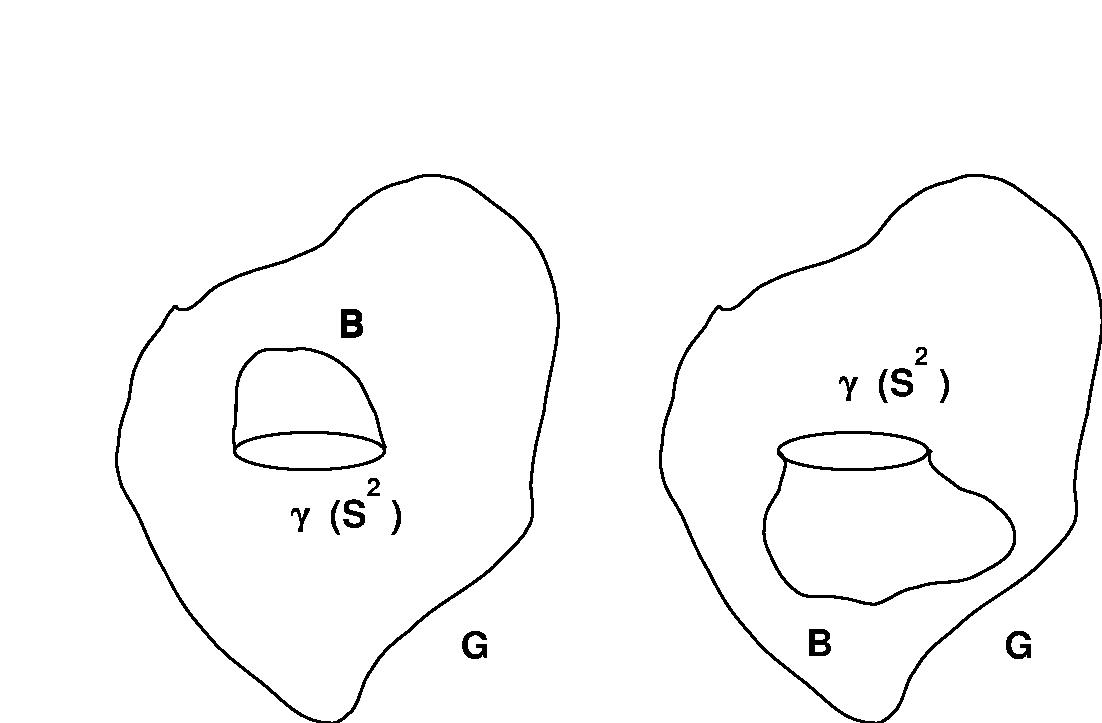
\includegraphics[width=100mm]{fig3}  
  \caption{Два продолжения поля на трехмерное многообразие}
  \label{fig:1}
\end{figure}

Разность значений члена Весса-Зумино $\Delta\Gamma$ на этих многообразиях
дается правой частью уравнения (\ref{eq:73}) с интегралом, продолженным на все компактное трехмерное
пространство. Так как оно топологически эквивалентно три-сфере, получаем
\begin{equation}
  \label{eq:75} \Delta\Gamma= - \frac{i }{24\pi} \int_{S^3}\epsilon_{ijk} Tr'\left( \tilde
g^{-1}\frac{\partial \tilde g}{\partial y^i} \tilde g^{-1}\frac{\partial \tilde g}{\partial y^j}
\tilde g^{-1}\frac{\partial \tilde g}{\partial y^k}\right) d^3y
\end{equation}
$\Delta\Gamma$ определен по модулю $2\pi i$, поэтому Евклидов функциональный интеграл
с весом $exp(-\Gamma)$ хорошо определен. Значит константа связи, умножаемая на этот член, должна
быть целочисленной.

Уравнение движения для полного действия (\ref{eq:4}):
\begin{equation}
  \label{eq:77}
  \partial^{\mu}(g^{-1}\partial_{\mu}g)+\frac{a^2 ik}{4\pi}\epsilon_{\mu\nu}\partial^{\mu}(g^{-1}\partial^{\nu}g)=0
\end{equation}
В комплексных координатах оно записывается в виде
\begin{equation}
  \label{eq:78}
  (1+\frac{a^2 k}{4\pi})\partial_z(g^{-1}\partial_{\bar z}g)+(1-\frac{a^2 k}{4\pi})\partial_{\bar z}(g^{-1}\partial_z g)=0
\end{equation}
Видно, что при $a^2=\frac{4\pi}{k}$ у нас имеются законы сохранения
\begin{equation}
  \label{eq:79}
  \partial_z(g^{-1}\partial{\bar z}g)=0
\end{equation}
Для токов
\begin{equation}
  \label{eq:72}
  J_z=\partial_z g\;g^{-1}, \qquad J_{\bar{z}}=g^{-1}\partial{\bar z}g
\end{equation}

\begin{equation}
  \label{eq:100}
  \partial_{\bar z}J=0,\quad \partial_z \bar J=0
\end{equation}
То есть голоморфная и антиголоморфная части отщепляются, что является указанием на наличие
конформной инвариантности.

Решение классического уравнения движения имеет вид
\begin{equation}
  \label{eq:80}
  g(z,\bar z)=f(z)\bar f(\bar z)
\end{equation}
при произвольных $f(z)$ и $\bar f (\bar z)$.

Сохранение по отдельности токов $J_z,\; J_{\bar z}$ приводит к инвариантности действия при преобразованиях
\begin{equation}
  \label{eq:81}
   g(z,\bar z)\to \Omega(z)g(z,\bar z)\bar \Omega^{-1}(\bar z)
\end{equation}
где $\Omega,\;\bar \Omega \in G$. То есть мы получили локальную $G(z)\times G(\bar z)$-инвариантность.

Для перехода к квантовому случаю мы переопределяем токи
\begin{equation}
  \label{eq:82}
  J(z)\equiv -k \partial_zg g^{-1}\quad \bar J(\bar z)=k g^{-1}\partial_{\bar z}g
\end{equation}
 При инфинитезимальных преобразованиях $\Omega=1+\omega,\; \bar \Omega =1+\bar \omega$ вариация
 $\delta_{\omega}g=\omega g$, а вариация действия
 \begin{equation}
   \label{eq:11}
   \delta S=-\frac{1}{2\pi}\int d^2 x \left(\partial_{\bar z}Tr(\omega(z)J(z))+\partial_z Tr(\bar
     \omega(\bar z)\bar J(\bar z))\right)
 \end{equation}
Заменяем $d^2 x=-\frac{i}{2} dz d\bar z$, интегрируем по частям и переходим к интегралу по контуру, замыкая
контур в разных направлениях для голоморфной и антиголоморфной частей.
Тогда вариация действия
\begin{equation}
  \label{eq:83}
  \delta_{\omega,\bar\omega}S=\frac{i}{4\pi}\oint dz Tr (\omega(z)J(z))-\frac{i}{4\pi}\oint d\bar z Tr(\bar\omega(\bar z)\bar J(\bar z))
\end{equation}
Раскладывая токи
\begin{equation}
  \label{eq:85}
  \begin{aligned}
    J=\sum J^a t^a,\bar J=\sum \bar J^a t^a \\
    \omega=\sum \omega^a t^a\\
  \end{aligned}
\end{equation}
получаем
\begin{equation}
  \label{eq:86}
  \delta_{\omega,\bar \omega}S=-\frac{1}{2\pi i}\oint dz \sum\omega^a J^a+\frac{1}{2\pi i} \oint d\bar z \sum \bar \omega^a \bar J^a
\end{equation}
Мы также получили тождества Уорда $\delta\left< X\right>=\left<(\delta S)X\right>$
\begin{equation}
  \label{eq:87}
  \delta_{\omega,\bar \omega}\left< X \right>=-\frac{1}{2\pi i}\oint dz \sum\omega^a \left< J^a X\right>+
  \frac{1}{2\pi i} \oint d\bar z \sum \bar \omega^a \left< \bar J^a X\right>
\end{equation}
Для токов из явного вида тока и формулы для преобразования $g$ имеем
\begin{equation}
  \label{eq:88}
  \delta_{\omega}J=[\omega,J]-k\partial_z\omega,\quad \delta_{\omega}J^a=\sum i f_{abc}\omega^b J^c-k\partial_z\omega^a
\end{equation}
Если это подставить в тождество Уорда, то получаем операторное разложение для токов, которое имеет
вид 
\begin{equation}
  \label{eq:89}
  J^a(z) J^b(w) \sim \frac{k\delta_{ab}}{(z-w)^2}+\sum i f_{abc}\frac{J^c(w)}{(z-w)}
\end{equation}
Раскладывая токи в ряд, получаем
\begin{equation}
  \label{eq:90}
  \begin{aligned}
    J^a(z)=\sum_{n\in \mathbb Z}z^{n-1}J^a_n\\
    \left[J^a_n,J^b_m\right]=\sum_c i f^{abc}J^c_{n+m}+kn\delta^{ab}\delta_{n+m,0}
  \end{aligned}
\end{equation}
Теперь мы видим, что компоненты токов образуют аффинную алгебру Ли $\hat g$.


Тензор энергии-импульса вводится при помощи конструкции Сугавары как сумма нормально упорядоченных компонент токов
\begin{equation}
  \label{eq:102}
  T(z)=\frac{1}{2(k+h^v)}\sum_a N(J^a J^a)(z)
\end{equation}
Здесь $h^v$ - дуальное число Кокстера. $h^v=\sum_i \alpha_i^v +1=\frac{1}{2}(\Theta,\Theta+2\rho)$,
а нормальное упорядочение вводится следующим образом: 
\begin{equation}
  \label{eq:12}
  N(AB)(w)=\frac{1}{2\pi i}\oint\frac{dz}{z-w}A(z)B(w)
\end{equation}

Тензор энергии-импульса можно разложить на моды $L_n$
\begin{equation}
  \label{eq:91}
  L_n=\frac{1}{2(k+h^v)}\sum_a\sum_m:J^a_m J^a_{n-m}:
\end{equation}
Тогда коммутационные соотношения для мод $L_n$ имеют вид
\begin{equation}
  \label{eq:92}
  \begin{aligned}
    \left[L_n,L_m\right]=(n-m)L_{n+m}+\frac{c}{12}(n^3-n)\delta_{n+m,0}\\
    c=\frac{k\;\mathrm{dim}g}{k+h^v}\\
    \left[L_n,J^a_m\right]=-mJ^a_{n+m}.
  \end{aligned}
\end{equation}

Таким образом, конструкция Сугавары --- это способ вложения алгебры Вирасоро в универсальную обертывающую аффинной алгебры Ли $\hat{g}$

Полная киральная алгебра модели Весса-Зумино-Виттена равна полупрямому произведению $Vir\ltimes \hat g$

Примарными оказываются поля, которые преобразуются ковариантно под действием $G(z)\times G(\bar z)$,
как $g(z,\bar z)$. В терминах операторного разложения это свойство переформулируется следующим
образом:
\begin{equation}
  \label{eq:84}
  \begin{aligned}
    J^a(z)g(w,\bar w)\sim \frac{-t^a g(w,\bar w)}{(z-w)}\\
    \bar J^a(z)g(w,\bar w)\sim \frac{ g(w,\bar w)t^a}{(z-w)}
  \end{aligned}
\end{equation}
Любое поле $\phi_{\lambda,\mu}$, преобразующееся ковариантно по отношению к некоторому
представлению, заданному весом $\lambda$ в голоморфном секторе и весом $\mu$ в антиголоморфном,
является примарным полем WZW-модели.

В модах это свойство записывается в виде
\begin{equation}
  \label{eq:93}
  \begin{aligned}
    & (J_0^a \phi_{\lambda})=-t^a_{\lambda}\phi_{\lambda}\\
    & (J^a_n\phi_{\lambda})=0\quad \mbox{для}\; n>0\\
  \end{aligned}
\end{equation}
Мы можем сопоставить состояние $\left|\phi_{\lambda}\right>$ полю $\phi_{\lambda}$
  \begin{equation}
    \label{eq:94}
    \phi_{\lambda}(0)=\left|\phi_{\lambda}\right>
  \end{equation}
Тогда условия (\ref{eq:93}) для примарных полей дают
\begin{equation}
  \label{eq:95}
  \begin{aligned}
    & J_0^a\left|\phi_{\lambda}\right>=-t^a_{\lambda}\left|\phi_{\lambda}\right>\\
    & J^a_n\left|\phi_{\lambda}\right>=0 \quad \mbox{для}\; n>0 \\
  \end{aligned}
\end{equation}
Все вторичные состояния имеют вид
\begin{equation}
  \label{eq:97}
  J^{a_1}_{-n_1}J^{a_2}_{n_2}\dots\left|\phi_{\lambda}\right>
\end{equation}

Легко видеть, что действие генераторов алгебры Вирасоро на примарные поля имеет вид
\begin{equation}
  \label{eq:96}
  L_0\left|\phi_{\lambda}\right>=\frac{1}{2(k+h^v)}\sum_aJ^a_0J^a_0\left|\phi_{\lambda}\right>=\frac{(\lambda,\lambda+2\rho)}{2(k+h^v)}\left|\phi_{\lambda}\right>
\end{equation}
Здесь использовано явное выражение для собственных значений квадратичного оператора Казимира.

Примарные поля преобразуются  интегрируемыми конечномерными представлениями, а бесконечномерные и
неинтегрируемые поля зануляют корреляционные функции.
В WZW-моделях примарные поля
принадлежат тензорному произведению неприводимых представлений аффинной алгебры, так как есть
голоморфный и антиголоморфный сектора.


\subsection{Конформные вложения и модулярно-инвариантные статсуммы}
\label{sec:modular-invariance}

При изучении конформной теории поля на плоскости или на сфере 
голоморфный и антиголоморфный сектора можно рассматривать независимо. 
Если мы говорим о применении конформной теории для описания поведения струн, то теория должна быть
определена на римановых поверхностях большего рода ($h>0$), чтобы можно было описывать
взаимодействия струн. Считается, что для этого необходимо (и, возможно, достаточно) чтобы теория была определена на торе.

(Нарисовать картинку штанов).

В теории критического поведения конформная инвариантность имеет место только в критической точке,
где голоморфный и антиголоморфный сектора расцеплены. Но вблизи критической точки эти сектора должны
быть связаны, и так как мы предполагаем плавный переход к критической точке в пространстве
параметров, то эта связь должна сохраняться и в критической точке. Физический спектр теории должен
плавно меняться, когда мы покидаем критическую точку, и связь голоморфного и антиголоморфного
сектора вдали от критической точки должна приводить к ограничениям на набор состояний в критической
точке. Этого можно достичь через геометрию, то есть накладывая граничные условия на состояния. Здесь
естественно рассматривать периодические граничные условия, которые эквивалентны рассмотрению теории
на торе.

%% Наложим периодические граничные условия с периодами $\omega_1, \omega_2,\; \tau=\omega_2/\omega_1$. 
%% Мы хотим вычислить статсумму для теории на торе через генераторы алгебры Вирасоро $L_0,\bar L_0$ и
%% выяснить ее зависимость от параметра $\tau$. Пусть пространственное направление соответствует
%% вещественной оси, а временное - мнимой. Пусть $\omega_1$ направлен вдоль вещественной оси. Через $H$
%% обозначим гамильтониан, а через $P$ - общий импульс системы. Тогда оператор трансляции на $a$
%% параллельно периоду $\omega_2$ имеет вид $\exp(-\frac{a}{|\omega_2|}(H \mathrm{Im} \omega_2-i P \mathrm{Re} \omega_2))$. 
%% Если считать, что $a$ - расстояние в решетке, то такой сдвиг переводит нас с одного ряда на другой
%% параллельно периоду $\omega_2$. Если полный период содержит $m$ ячеек решетки ($|\omega_2|=ma$), то
%% статсумма дается следом оператора сдвига в степени $m$:
%% \begin{equation}
%%   \label{eq:6}
%%   Z(\omega_1,\omega_2)=\mathrm{Tr} \exp-\{H \mathrm{Im} \omega_2-iP\mathrm{Re}\omega_2\}
%% \end{equation}
%% Операторы $H,P$ можно выразить через генераторы алгебры Вирасоро если рассмотреть тор как цилиндр
%% конечной длины со склеенными концами. На цилиндре с длиной окружности $L$ гамильтониан
%% $H=(2\pi/L)(L_0+\bar L_0-c/12)$. Константа добавлена, чтобы вакуумная энергия исчезала в пределе
%% $L\to \infty$. Оператор импульса, который генерирует трансляции вокруг окружности, имеет вид
%% $P=(2\pi i/L)(L_0-\bar L_0)$. Так как мы выбрали $\omega_1$ вещественным и равным $L$, статсумму
%% можно записать в виде
%% \begin{equation}
%%   \label{eq:7}
%%   \begin{split}
%%       Z(\tau)=\mathrm{Tr}\exp \pi i \{(\tau-\bar \tau)(L_0+\bar L_0-c/12)+(\tau+\bar \tau)(L_0-\bar
%%       L_0)\}\\
%%       =\mathrm{Tr} \exp 2 \pi i \{\tau(L_0-c/24)-\bar\tau (\bar L_0-c/24)\}\\
%%   \end{split}
%% \end{equation}
%% Или, если ввести $q=\exp 2\pi i \tau$
%% \begin{equation}
%%   \label{eq:2}
%%   Z(\tau)=Tr \left (q^{L_0-c/24}\bar{q}^{\bar{L}_0-c/24}\right)
%% \end{equation}
%% Это выражение, на самом деле --- сумма характеров представлений алгебры Вирасоро (конформных семейств).
%% 
%% Двумерный тор представляет собой фактор пространство $\mathbb{R}^2\approx \mathbb{C}$ по отношениям
%% эквивалентности $z\sim z+w_1$ and $z\sim z+w_2$, где $w_1$ и $w_2$ не параллельны.
%% 
Разные параметризации тора связаны модулярными преобразованиями, таким образом возникает требование
модулярной инвариантности статсуммы.

При помощи конформных преобразований можно перейти к таким координатам, в которых соотношения
эквивалентности для тора (граничные условия) записываются в виде $z\sim z+1$ и $z\sim z+\tau$, где $\tau$ в верхней полуплоскости
$\mathbb{C}$.
%% 
%% Легко видеть, что $\tau$, $T(\tau)=\tau+1$ и $S(\tau)=-\frac{1}{\tau}$ описывают
%% конформно-эквивалентные торы. Отображения $T$ и $S$ порождают группу
%% $SL(2,\mathbb{Z})/\mathbb{Z}_2$, состоящую из матриц вида
%% \begin{equation}
%%   \label{eq:99} A=
%%   \begin{pmatrix} a & b\\ c & d
%%   \end{pmatrix} \quad\mbox{где}\; a,b,c,d\in\mathbb{Z},\quad ad-bc=1,
%% \end{equation}
%% и матрицы $A$ и $-A$ действуют одинаково на $\tau$
%% \begin{equation}
%%   \label{eq:100} \tau\to A\tau=\frac{a\tau+b}{c\tau+d}
%% \end{equation}
%% $\tau$ называется модулярным параметром, а группа $SL(2,\mathbb{Z})/\mathbb{Z}_2$ ---
%% модулярной группой.
%% 
Конформная теория поля задаётся примарными полями $\Phi_a$ с конформными размерностями $\Delta_a$.

Примарные поля живут в пространствах $\mathcal{H}_{(i,j)}$, которые представляют собой тензорные
произведения неприводимого представления $\mathcal{H}_j$ киральной алгебры и неприводимого
представления $\bar{\mathcal{H}}_{\bar{j}}$ антикиральной алгебры. Тогда статсумма на торе
(\ref{eq:2}) может быть записана в виде
\begin{equation}
  \label{eq:9}
    Z(\tau)=\sum_{(j,\bar j)}\chi_j(q)\bar \chi_{\bar j}(\bar q)
\end{equation}
где $\chi_j$ --- нормализованный характер представления $\mathcal{H}_j$,
\begin{equation}
  \label{eq:5} \chi_j(\tau)=Tr_{\mathcal{H}_j}(q^{L_0-\frac{c}{24}})\quad \mbox{где}\; q=e^{2\pi i
\tau}
\end{equation}

Характеры переходят друг в друга при модулярных преобразованиях:
\begin{equation}
  \label{eq:107} \chi_j\left(-\frac{1}{\tau}\right)=\sum_k S_{jk}\chi_k(\tau)\quad \mbox{и}\quad
\chi_j(\tau+1)=\sum_kT_{jk}\chi_k(\tau),
\end{equation}
где $S$ и $T$ --- постоянные матрицы. 

Для WZW-моделей примарные поля определяются старшими весами  $\hat \lambda, \hat \xi$ соответствующих представлений алгебры $\mathfrak{g}$. Тогда
\begin{equation}
  \label{eq:6} \mathcal{H}=\bigoplus_{\hat \lambda,\hat \xi\in P^{(k)}_{+}}M_{\hat \lambda,\hat \xi}
L_{\hat \lambda}\otimes L_{\hat \xi}
\end{equation}

Коэффициенты ветвления для вложения аффинной подалгебры Ли в аффинную алгебру можно использовать для
построения модулярно-инвариантной статсуммы в соответствующей WZW-модели. Когда рассматривается
теория на торе,  набор физически допустимых полей ограничен требованиями модулярной инвариантности.

Простейший модулярный инвариант можно записать следующим образом:
\begin{equation}
  \label{eq:34}
   Z(\tau)=\sum_{ \mu\in P^{+}_{\mathfrak{g}}} \chi_{\mu}(\tau)\bar \chi_{\mu}(\bar \tau)
\end{equation}
Здесь суммирование ведется по всем конформным семействам (то есть по всем представлениям алгебры
$\mathfrak{a}$).

Другие модулярные инварианты в WZW-модели с алгеброй $\mathfrak{a}$ можно получить, если существует
алгебра $\mathfrak{g}$, в которую $\mathfrak{a}$ вкладывается конформно. (Я сейчас поясню, что это
значит). 

Представления алгебры можно рассматривать как сумму представлений подалгебры. 

Если мы рассмотрим редукцию характеров аффинной алгебры
\begin{equation}
  \label{eq:8}
   \pi_{\mathfrak{a}}(ch L^{\mu}_{\mathfrak{g}})=
  \sum_{\nu\in P^{+}_{\mathfrak{a}}}b^{(\mu)}_{\nu} ch L^{\nu}_{\mathfrak{a}}
\end{equation}
и подставим разложение в формулу \eqref{eq:34}, то модулярная инвариантность сохранится. То есть из
диагонального инварианта для алгебры $\mathfrak{g}$ мы получаем новый не диагональный инвариант для
подалгебры $\mathfrak{a}$. Но возникает вопрос, будет ли теория, полученная таким образом, самосогласованной, сохранится ли в
ней конформная инвариантность.

Пусть $J^{a_j}_{-n_j}$ и $\tilde{J}^{a'_j}_{-n_j}$ --- понижающие операторы алгебр  $\mathfrak{g}$ и
$\mathfrak{a}\subset\mathfrak{g}$.  $\pi_{\mathfrak{a}}$ --- проекционный оператор
$\pi_{\mathfrak{a}}:\mathfrak{g}\longrightarrow \mathfrak{a}$. В теории, связанной с  $\mathfrak{g}$
с вакуумом $\left|\lambda\right>$ будут следующие состояния:
\begin{equation}
  \label{eq:109}
  J^{a_1}_{-n_1}J^{a_2}_{-n_2}\dots\left|\lambda\right>\quad n_1\geq n_2\geq \dots>0.
\end{equation}
Вакуум $\mathfrak{g}$-инвариантен, то есть $J_0^a\left|0\right>=0$. При проекции на подалгебру
$\mathfrak{a}$ состояния примут вид
\begin{equation}
  \label{eq:110}
  \tilde{J}^{a'_1}_{-n_1}\tilde{J}^{a'_2}_{-n_2}\dots\left|\pi_{\mathfrak{a}}(\lambda)\right>.
\end{equation}
Из $\mathfrak{g}$-ивариантности вакуума следует его $\mathfrak{a}$-инвариантность, но для тензора
энергии-импульса в общем случае это не так. Поэтому тензор энергии-импульса большей теории должен
состоять только из генераторов $\tilde{J}$. Тогда $T_{\mathfrak{g}}=T_{\mathfrak{a}}\Rightarrow
c(\mathfrak{g})=c(\mathfrak{a})$. Это приводит к уравнению
\begin{equation}
  \label{eq:111}
  \frac{k\;\mathrm{dim}\,\mathfrak{g}}{k+g}=\frac{x_e k\; \mathrm{dim}\,\mathfrak{a}}{x_ek+a}
\end{equation}
Здесь $x_e$ --- индекс вложения, а  $g$, $a$ --- дуальные числа Кокстера, которые характеризуют алгебры.

Можно показать, что только для представлений уровня 1 это равенство удовлетворяется. То есть класс
конформных вложений не слишком широк и существует полная их классификация. Кроме того, для
конформных вложений существуют специальные методы разложения представлений.

Модулярная инвариантность статсуммы для полей, принадлежащих представлениям алгебры  $\mathfrak{g}$,
сохраняется при проекции на подалгебру $\mathfrak{a}$. Если все представления $\mathfrak{g}$ в теории
удовлетворяют описанным требованиям, то при проекции мы получаем конформную теорию поля.

Существует теорема о том, что для конформного вложения  $\mathfrak{a}\subset\mathfrak{g}$ только
конечное число коэффициентов ветвления отлично от нуля. Поэтому после того, как мы разложили все
представления $\mathfrak{g}$ мы подставляем результаты в выражение для статсуммы и получаем
модулярно-инвариантную статсумму для вложенной теории. Такая статсумма уже не будет иметь
диагональный вид:
\begin{equation}
  \label{eq:36}
   Z_{\mathfrak{a}}(\tau)=\sum_{ \nu,\lambda\in P^{+}_{\mathfrak{a}}} \chi_{\nu}(\tau)M_{\nu\lambda}\bar \chi_{\lambda}(\bar \tau)
\end{equation}
Наша работа посвящена разработке общего метода редукции представлений аффинных алгебр Ли, поэтому
случай конформных вложений --- лишь один из примеров применения нашего метода. Однако в этом случае
физический смысл наиболее очевиден. 





%%
%% End of file
%%% Local Variables: 
%%% mode: latex
%%% TeX-master: "thesis"
%%% End: 


\chapter{Разложение сингулярных элементов и рекуррентные соотношения для коэффициентов ветвления}
\label{cha:affine-lie-algebras}

В главе \ref{cha:CFT} мы показали, что для построения модулярно-инвариантных статсумм и в процессе изучения coset-моделей возникает проблема ветвления для аффинных алгебр Ли.  В данной главе мы выводим рекуррентные соотношения на коэффициенты ветвления, которые являеются важнейшим инструментом данной диссертации. Эти соотношения получены нами в работе \cite{2010arXiv1007.0318L}.

Существуют различные подходы к вычислению коэффициентов ветвления. Некоторые из них используют резольвенту Бернштейна-Гельфанда-Гельфанда \cite{bernstein1975differential} (См. главу \ref{cha:BGG}, алгоритм вычислений описан в работах \cite{kac1990idl},\cite{wakimoto2001idl}), ряды функций Шура \cite{fauser2006new}, когомологии БРСТ  \cite{Hwang:1994yr}, формулы Каца-Петерсона  \cite{kac1990idl,quella2002branching} или комбинаторные методы \cite{feigin707principal}.

В этой главе мы доказываем, что для произвольной редуктивной подалгебры коэффициенты ветвления описываются набором рекуррентных соотношений и существует эффективный и простой алгоритм для пошагового решения этих соотношений. Общая идея похожа на подход, предложенный в работе  \cite{ilyin812pbc} для максимальных вложений. Но в данном случае алгоритм существенно отличается, так как использует новые свойства сингулярных весов для работы с произвольными редуктивными вложениями $\af \rightarrow \gf$.

При этом важно рассматривать подалгебру  $\af$ вместе с ее ``ортогональным партнером'' $\afb\subset \gf$. 
Для любой редуктивной подалгебры $\af$ подалгебра $\afb$ регулярна и редуктивна. 

Для модуля старшего веса  $L^{\left( \mu \right)}$ и ортогональной пары подалгебр $\left(  \af, \afb \right)$ мы рассматриваем так называемый сингулярный элемент  $\Psi^{\left( \mu \right)}$ (числитель в формуле Вейля для характеров
$ch\left( L^{\mu }\right) =\frac{\Psi ^{\left( \mu \right) }}{\Psi ^{\left( 0\right) }}$,
см., например, \cite{humphreys1997introduction}), 
знаменатель Вейля $\Psi ^{\left( 0\right) }_{\afb}$ и проекцию
$\Psi ^{\left( \mu \right) }_{\left(  \af, \afb \right)}
=\pi_{\af}\frac{\Psi ^{\left( \mu \right) }_{\gf}}{\Psi ^{\left( 0\right) }_{\afb}}$.

Мы доказываем, что для произвольного $\hf$-диагонализующего модуля старшего веса $L^{\left( \mu \right)}$ и ортогональной пары $\left(  \af, \afb \right)$ элемент
$\Psi ^{\left( \mu \right) }_{\left(  \af, \afb \right)}$ допускает разложение на множество числителей Вейля $\Psi ^{\left( \mu \right) }_{ \afb }$ модулей подалгебры $\afb$.
Это разложение дает возможность построить рекуррентное соотношение для коэффициентов ветвления, соответствующих вложению $\af \rightarrow \gf $. Рекуррентное соотношение формулируется с использованием особого элемента  $\Gamma_{\af \rightarrow \gf}$ групповой алгебры
$\mathcal{E}\left( \gf \right)$, который мы называем ``веером вложения''. 
Применение этих инструментов позволяет нам сформулировать простой и явный алгоритм для вычисления коэффициентов ветвления, который может быть использован в случае произвольных (максимальных и не максимальных) подалгебр конечномерных и аффинных алгебр Ли. 
В случае максимального вложения веер имеет простую форму, сингулярный элемент становится тривиальном $\Psi ^{\left( \mu \right) }_{\left(  \af, \afb \right)}=\Psi ^{\left( \mu \right) }_{\left(  \gf\right)}$ и мы восстанавливаем соотношения, полученные ранее в работе \cite{ilyin812pbc}.

Также мы показываем, что предложенный алгоритм эффективен и может использоваться при изучении конформных вложений и coset-моделей в рациональной конформной теории поля.

В разделе \ref{sec:branching} мы выводим формулы разложения, основывающиеся на аномальных коэффициентах ветвления и описываем алгоритм редукции интегрируемых модулей старшего веса $L_{\mathfrak{g}}$ по отношению к редуктивной подалгебре  $\mathfrak{a}\subset \mathfrak{g}$. В разделе \ref{sec:branching-examples} мы представляем различные примеры применения алгоритма для конечномерных (\ref{sec:finite-dimens-lie}) и аффинных алгебр Ли и обсуждаем их роль в моделях конформной теории поля (\ref{sec:phys-appl}). Выводы к главе изложены в разделе \ref{sec:conclusion}. В следующей главе \ref{cha:BGG} мы показываем связь процедуры редукции с обобщенной резольвентой Бернштейна-Гельфанда-Гельфанда.  Реализация алгоритма на языке {\it Mathematica} и дополнительные примеры машинных вычислений описаны в разделе \ref{cha:computational-methods} главы \ref{cha:applications}. 


\section{Рекуррентные соотношения для коэффициентов ветвления}
\label{sec:branching}

Рассмотрим интегрируемый модуль $L^{\mu }$ алгебры $\gf$ со старшим весом  $\mu$ и пусть  $\af\subset\gf$ -- редуктивная подалгебра $\gf$. Модуль $L^{\mu}$ вполне приводим по отношению к $\af$.
\begin{equation*}
 L_{\gf\downarrow \af}^{\mu }=\bigoplus
\limits_{\nu \in P_{\af}^{+}}b_{\nu }^{\left( \mu \right) }L_{\af}^{\nu }.
\end{equation*}
Используем оператор проекции  $\pi_{\af}$ (на весовое пространство $\hf_{\af}^*$) и перепишем это разложение в терминах формальных характеров:
\begin{equation}
\label{branching1}
 \pi _{\af}\circ ch\left( L^{\mu }\right)
 =\sum_{\nu \in P_{\af}^{+}}b_{\nu }^{(\mu)}ch\left( L_{\af}^{\nu }\right) .
\end{equation}
Нас интересуют коэффициенты ветвления $b^{(\mu)}_{\nu}$.

\subsubsection{Ортогональная подалгебра и веер вложения.}
\label{subsec:branching-orthog-pair}

В этой секции мы введем простые конструкции, которые будут полезны при изучении ветвлений. Важный объект здесь -- это ``ортогональный партнер''  $\afb$ редуктивной подалгебры $\af$ в  $\gf$.

В формуле Вейля-Каца \eqref{eq:13} и числитель, и знаменатель могут рассматриваться как формальные элементы, содержащие сингулярные веса модулей Верма $V^{\xi}$ со старшими весами  $\xi=\mu$ и $\xi=0$ \cite{humphreys1997introduction}.
Мы связываем сингулярные элементы с соответствующими интегрируемыми модулями  $L^{\mu }$ и $L_{\af}^{\nu }$:
\begin{equation*}
\Psi ^{\left( \mu \right) }:=\sum\limits_{w\in W}\epsilon (w)e^{w\circ (\mu +\rho )-\rho },
\end{equation*}
\begin{equation*}
\Psi _{ \af}^{\left( \nu \right) }:= \sum\limits_{w\in W_{\af}}\epsilon (w)e^{w\circ (\nu +\rho_{_{\af}})-\rho _{_{\af}}}.
\end{equation*}
и используем формулы Вейля-Каца в форме
\begin{equation}
\label{Weyl-Kac2}
ch\left( L^{\mu }\right) =\frac{\Psi ^{\left( \mu \right) }}{\Psi ^{\left( 0 \right) }}=\frac{\Psi ^{\left( \mu \right) }}{R}.
\end{equation}

Применим формулу  (\ref{Weyl-Kac2}) к правилу ветвления (\ref{branching1}) и получим соотношение, связывающее сингулярные элементы
 $\Psi ^{\left( \mu \right) }$ and $\Psi _{ \af}^{\left( \nu \right) }$ :
\begin{eqnarray}
\nonumber
\pi _{\af}\left( \frac{\sum_{w \in W}\epsilon (w )e^{w
(\mu +\rho )-\rho }}{\prod_{\alpha \in \Delta ^{+}}(1-e^{-\alpha })^{\mathrm{%
mult}(\alpha )}}\right) &=&\sum_{\nu \in P_{\af}^{+}}b_{\nu }^{(\mu )}%
\frac{\sum_{w \in W_{\af}}\epsilon (w )e^{w (\nu +\rho _{%
\af})-\rho _{\af}}}{\prod_{\beta \in \Delta _{\af%
}^{+}}(1-e^{-\beta })^{\mathrm{mult}_{\af}(\beta )}},  \label{eq:124} \\
\pi _{\af}\left( \frac{\Psi ^{\left( \mu \right) }}{R}\right)
&=&\sum_{\nu \in P_{\af}^{+}}b_{\nu }^{(\mu )}\frac{\Psi _{ \frak{%
a}}^{\left( \nu \right) }}{R_{\af}}.
\end{eqnarray}
Здесь $\Delta _{\af}^{+}$ -- множество положительных корней подалгебры $\af$ (без потери общности мы можем считать их векторами из положительного корневого пространства  $\hf^{\ast  +}$ алгебры $\gf$).

Рассмотрим корневое подпространство $\hf_{\perp \af}^{\ast }$, ортогональное к  $\af$,
\begin{equation*}
\hf_{\perp \af}^{\ast }:=\left\{ \eta \in \hf^{\ast }
|\forall h \in \hf_{\af};  \eta\left(h \right)=0 \right\} ,
\end{equation*}
и корни (соответственно -- положительные корни)  $\gf$, ортогональные
к $\af$,
\begin{eqnarray}
\label{delta-a-ort}
\Delta _{\af_{\perp }} &:&=\left\{ \beta \in \Delta _{\gf}|
\forall h \in \hf_{\af};  \beta\left(h \right)=0  \right\} , \\
\Delta _{\af_{\perp }}^{+} &:&=\left\{ \beta ^{+}\in \Delta _{\gf%
}^{+}|\forall h \in \hf_{\af};  \beta^{+}\left(h \right)=0  \right\} .
\end{eqnarray}
Обозначим через $W_{\afb}$ подгруппу группы Вейля $W$, порожденную отражениями $w _{\beta }$, соответствующими корням $\beta \in \Delta _{\afb}^{+}$ . Подсистема  $\Delta _{\af_{\perp }}$ определяет подалгебру $\af_{\perp }$ с подалгеброй Картана $\hf_{\afb}$. Пусть
\begin{equation*}
\hf_{\perp }^{\ast }:=\left\{ \eta \in \hf_{\perp \af}^{\ast
}|\forall h \in \hf_{\af\oplus \af_{\perp}}; \eta \left( h \right)=0 \right\},
\end{equation*}
рассмотрим подалгебры
\begin{eqnarray*}
\widetilde{\af_{\perp }} &:&=\af_{\perp }\oplus \hf_{\perp }
\\
\widetilde{\af} &:&=\af\oplus \hf_{\perp }.
\end{eqnarray*}
Алгебры $\af$ и $\af_{\perp }$ образуют ''ортогональную пару''
$\left( \af,\afb\right)$ подалгебр в  $\gf$.

Имеет место разложение подалгебры Картана
\begin{equation}
\hf=\frak{\hf_{\af}}\oplus \hf_{\afb}\oplus
\hf_{\perp }=\frak{\hf_{\widetilde{\af}}}\oplus \hf_{\afb}=\frak{\hf_{\widetilde{\afb}}}\oplus
\hf_{\af}.
\end{equation}

Для подалгебр из ортогональной пары  $\left( \af,\afb\right) $ рассмотрим соответствующие векторы Вейля $\rho _{\af}$ и $\rho _{\af_{\perp }}$, и образуем так называемые  ''дефекты'' вложения $\mathcal{D}_{\af}$ и $\mathcal{D}_{\af_{\perp }}$ :
\begin{equation}
\mathcal{D}_{\af}:=\rho _{\af}-\pi _{\af}\rho ,
\end{equation}
\begin{equation}
\label{defect-perp}
\mathcal{D}_{\af_{\perp }}:=\rho _{\af_{\perp }}-\pi_{\afb}\rho .
\end{equation}

Рассмотрим сингулярные веса  $\left\{\left( w(\mu +\rho )-\rho \right)|w  \in W \right\}$  модуля старшего веса  $L_{\gf}^{\mu }$ и их проекции на $h_{\widetilde{\af_{\perp }}}^{\ast }$ (дополнительно сдвинутые на дефект $-\mathcal{D}_{\af_{\perp }}$):
\begin{equation*}
\mu _{\widetilde{\af_{\perp }}}\left( w\right) :=\pi _{\widetilde{\frak{%
a}_{\perp }}}\circ\left[ w(\mu +\rho )-\rho \right] -\mathcal{D}_{\af_{\perp
}},\quad w\in W.
\end{equation*}
Среди весов  $\left\{\mu _{\widetilde{\af_{\perp }}}\left( w\right)|w\in W\right\}$ выберем находящиеся в главной камере Вейля $\overline{C_{\widetilde{\afb}}}$ и обозначим через $U$ множество представителей $u$ классов смежности $W/W_{\af_{\perp }}$, таких что
\begin{equation}
U:=\left\{ u\in W|\quad \mu _{\widetilde{\af_{\perp }}}\left( u\right)
\in \overline{C_{\widetilde{\af_{\perp }}}}\right\} \quad .
\label{U-def}
\end{equation}
Для множества  $U$ введем веса
\begin{equation*}
\mu _{\af}\left( u\right) :=\pi _{\af}\circ\left[ u(\mu +\rho )-\rho %
\right] +\mathcal{D}_{\af_{\perp }}.
\end{equation*}
Кроме того, мы будем пользоваться аналогичным определением
\begin{eqnarray}
\label{eq:136}
\mu _{\tilde \af}\left( u\right) :=\pi _{\tilde \af}\left[ u(\mu +\rho )-\rho \right] +\mathcal{D}_{\afb},\\
\mu _{\afb}\left( u\right) :=\pi _{\afb}\left[ u(\mu +\rho )-\rho \right] +\mathcal{D}_{\afb}.
\end{eqnarray}

Чтобы упростить вид соотношений мы будем опускать значок "$\circ$" при записи проекций весов.

Воспользуемся техникой, предложенной в работе  \cite{ilyin812pbc} для записи рекуррентных свойств коэффициентов ветвления $b_{\nu}^{(\mu )}$. Один из инструментов в ней -- это множество весов $\Gamma_{\af\rightarrow \gf}$, называющееся веером вложения. Так как мы рассматриваем общую ситуацию (где вложение не обязательно максимально) понятие веера вложения нуждается в уточнении:
\begin{definition}
\label{fan-definition} Рассмотрим произведение
\begin{equation}
\prod_{\alpha \in \Delta ^{+}\setminus \Delta _{\afb }^{+}}\left( 1-e^{-\pi
_{\af}\alpha }\right) ^{\mathrm{mult}(\alpha )-\mathrm{mult}_{\af%
}(\pi _{\af}\alpha )}=-\sum_{\gamma \in P_{\af}}s(\gamma
)e^{-\gamma }  \label{eq:142}
\end{equation}
и носитель $\Phi _{\af\subset \gf}\subset P_{\af}$ функции $s(\gamma )=\det \left( \gamma \right) $ :
\begin{equation}
\Phi _{\af\subset \gf}=\left\{ \gamma \in P_{\af}|s(\gamma
)\neq 0\right\}   \label{eq:37}
\end{equation}
Упорядочение корней в  $\co{\Delta _{\af}}$ индуцирует естественное упорядочение весов в $P_{\af}$. Обозначим через $\gamma_{0}$ наименьший вектор $\Phi _{\af\subset \gf}$. Множество
\begin{equation}
\Gamma _{\af\rightarrow \gf}=\left\{ \xi -\gamma _{0}|\xi \in \Phi _{%
\af\subset \gf}\right\} \setminus \left\{ 0\right\}
\label{fan-defined}
\end{equation}
называется  \textit{веером вложения}.
\end{definition}
В следующем разделе мы покажем, что веер вложения определяет рекуррентные свойства коэффициентов ветвления. Нужно отметить, что веер вложения универсален и зависит только от вложения. 

\subsubsection{Разложение сингулярного элемента.}
\label{subsec:decomp-sing-element}

Покажем, что формула Вейля-Каца для характеров (в терминах сингулярных элементов) представляет собой частный случай более общего соотношения:

\begin{lemma}
\label{lemma}
Пусть $\left( \af,\afb \right)$ -- ортогональная пара редуктивных подалгебр $\gf$ и  $\widetilde{\afb}=\afb\oplus \hf_{\perp }$, $\widetilde{\af}=\af\oplus\hf_{\perp }$ ,

$L^{\mu }$ -- модуль старшего веса с сингулярным элементом $\Psi ^{\left(\mu \right)}$ ,

$R_{\af_{\perp }}$ -- знаменатель Вейля для подалгебры $\af_{\perp }$.

Тогда элемент  $\Psi ^{\left( \mu \right) }_{\left(  \af, \afb \right)}=\pi _{\af}\left( \frac{\Psi _{\gf}^{\mu }}{R_{\af_{\perp }}}\right) $ можно разложить в сумму по  $u\in U$ (см. (\ref{U-def})) сингулярных весов $e^{\mu _{\af}\left( u\right) }$ с коэффициентами $\epsilon (u)\mathrm{\dim}\left( L_{\widetilde{\afb}}^{\mu _{\widetilde{\afb}}\left( u\right) }\right) $:
\begin{equation}
\Psi ^{\left( \mu \right) }_{\left(  \af, \afb \right)}=\quad \pi _{\af}\left( \frac{\Psi^{\mu }}{R_{\af%
_{\perp }}}\right) =\sum_{u\in U}\;\epsilon (u)\mathrm{\dim }
\left( L_{\widetilde{\af_{\perp }}}^{\mu _{%
\widetilde{\af_{\perp }}}\left( u\right) }\right) e^{\mu _{\af}\left( u \right) }.
\end{equation}
\end{lemma}

\begin{proof}
Для $u\in U $ и $v\in W_{\afb}$ применим разложение
\begin{equation*}
u(\mu +\rho )=\pi _{\af } u(\mu +\rho )+\pi _{
\widetilde{\af_{\perp }} } u(\mu +\rho )
\end{equation*}
к сингулярному весу
\begin{equation}
\label{sing-decomp-1}
\begin{array}{lcl}
vu(\mu +\rho )-\rho &=&\pi _{ \af }\left( u(\mu +\rho
)\right) -\rho +\rho _{\af_{\perp }}+\pi _{ \hfb }\rho \\
&& + \ v\left( \pi _{ \widetilde{%
\af_{\perp }} }u(\mu +\rho )-\rho _{\af_{\perp }}+\rho _{%
\af_{\perp }}\right) -\rho _{\af_{\perp }} -\pi _{ \hfb }\rho.
\end{array}
\end{equation}
Используем дефект $\mathcal{D}_{\afb}$ (\ref{defect-perp}) чтобы упростить в (\ref{sing-decomp-1}) первое слагаемое :
\begin{equation*}
\begin{array}{r}
\pi _{ \af }\left( u(\mu +\rho )\right) -\rho +\rho _{%
\mathfrak{a}_{\perp }}+\pi _{ \hfb }\rho = \\
\pi _{ \af }\left( u(\mu +\rho )\right) -\pi _{\af}\rho
-\pi _{\afb}\rho +\rho _{\afb}= \\
=\pi _{ \af }\left( u(\mu +\rho )-\rho \right) +%
\mathcal{D}_{\afb},
\end{array}
\end{equation*}
и второе:
\begin{equation*}
\begin{array}{c}
v\left( \pi _{ \widetilde{%
\af_{\perp }} }u(\mu +\rho )-\rho _{\af_{\perp }}+\rho _{%
\af_{\perp }}\right) -\rho _{\af_{\perp }}-\pi _{ \hfb }\rho=\\
v\left( \pi _{ \widetilde{%
\afb} }u(\mu +\rho )
- \mathcal{D}_{\afb} - \pi _{ \afb }\rho-\pi _{ \hfb }\rho
+\rho _{\afb}\right) -\rho _{\afb}=\\
=v\left( \pi _{ \widetilde{%
\afb} }\left[ u(\mu +\rho )-\rho\right]
- \mathcal{D}_{\afb}
+\rho _{\afb}\right) -\rho _{\afb}.
\end{array}
\end{equation*}
Эти выражения обеспечивают факторизацию сингулярного элемента  $\Psi^{\mu}$ и мы видим, что они содержат комбинации сингулярных элементов $\Psi _{\widetilde{\af_{\perp }}}^{\eta }$ модулей $L_{\widetilde{\afb}}^{\eta }$ подалгебры  $\widetilde{\afb}$:
\begin{equation*}
\begin{array}{l}
\Psi^{\mu }=\sum_{u\in U}\sum_{v\in W_{\af_{\perp }}}
\epsilon (v)\epsilon (u)e^{vu(\mu +\rho )-\rho }= \\
=\sum_{u\in U}\epsilon (u)e^{\pi _{\af}\left[ u(\mu +\rho )-\rho \right]
+\mathcal{D}_{\af_{\perp }}}\sum_{v\in W_{\af_{\perp }}}\epsilon
(v)e^{v\left( \pi _{ \widetilde{\af_{\perp }} }\left[
u(\mu +\rho )-\rho \right] -\mathcal{D}_{\af_{\perp }}+\rho _{\af%
_{\perp }}\right) -\rho _{\af_{\perp }}}= \\
=\sum_{u\in U}\;\epsilon (u)e^{\pi _{\af }\left[ u(\mu
+\rho )-\rho \right] +\mathcal{D}_{\af_{\perp }}}\Psi _{\widetilde{%
\af_{\perp }}}^{\pi _{ \widetilde{\af_{\perp }} }%
\left[ u(\mu +\rho )-\rho \right] -\mathcal{D}_{\af_{\perp }}}
\end{array}
\end{equation*}

Разделим обе части на элемент Вейля  $R_{\af_{\perp }}=\prod_{\beta \in \Delta _{\afb}}(1-e^{-\beta })^{\mathrm{mult}(\beta )}$, спроектируем их на весовое подпространство  $h_{\af}^{\ast }$ и получим итоговое соотношение:
\begin{eqnarray*}
\Psi ^{\left( \mu \right) }_{\left(  \af, \afb \right)}
&=&\sum_{u\in W/W_{\af_{\perp }}}\;\epsilon (u)e^{\pi _{\frak{a%
}}\left[ u(\mu +\rho )-\rho \right] }\pi _{%
\af}\left( \frac{\Psi _{\widetilde{\af_{\perp }}}^{\pi _{
\widetilde{\af_{\perp }} }\left[ u(\mu +\rho )-\rho \right] -%
\mathcal{D}_{\af_{\perp }}}}{\prod_{\beta \in \Delta _{\af_{\perp
}}}(1-e^{-\beta })^{\mathrm{mult}(\beta )}}\right)  \\
&=&\sum_{u\in U}\;\epsilon (u)\mathrm{\dim }\left( L_{\widetilde{\af%
_{\perp }}}^{\mu _{\widetilde{\af_{\perp }}}\left( u\right) }\right)
e^{\pi _{\af}\left[ u(\mu +\rho )-\rho \right] }.
\end{eqnarray*}
\end{proof}


\begin{remark}
Это соотношение можно рассматривать как обобщение формулы Вейля для сингулярного элемента  $\Psi _{\gf}^{\mu }$: векторы  $\mu_{\af}\left(u\right)$ играют роль сингулярных весов, но вместо определителей $\epsilon (u)$ появляются произведения  $\epsilon(u)\mathrm{\dim }\left( L_{\widetilde{\afb}}^{\mu _{\widetilde{\afb}}\left(u\right) }\right).$ Действительно, при  $\frak{a=g}$ подалгебры  $\afb$ и $\hf_{\perp }$ тривиальны, $U=W$ , и исходная формула Вейля с легкостью восстанавливается. 
\end{remark}

\subsubsection{Построение рекуррентных соотношений.}
\label{subsec:Construct-recurrent-rel}

Рассмотрим правую часть равенства (\ref{eq:124}).
Числитель описывает ветвление в терминах сингулярных элементов и, как элемент  $\mathcal{E}\left( \gf \right)$, допускает разложение в виде:
\begin{equation}
  \label{eq:21}
  \sum_{\nu \in \bar{C_{\mathfrak{a}}}}b_{\nu }^{\left( \mu \right) }\Psi _{\left( \frak{%
        a}\right) }^{\left( \nu \right) }=\sum_{\lambda \in P_{\af}}k_{\lambda
  }^{\left( \mu \right) }e^{\lambda }.
\end{equation}
Здесь $k_{\lambda}^{\left( \mu \right) }$  -- целочисленные коэффициенты, их знаки зависят от длины элементов группы Вейля в 
$\Psi _{\left( \af\right) }^{\left( \nu \right) }$. Важно заметить, что $k_{\lambda}^{\left( \mu \right) }$ совпадают с коэффициентами ветвления для всех весов $\nu$ в главной камере Вейля:
\begin{equation}
  \label{eq:119}
  b^{(\mu)}_{\nu}=k^{(\mu)}_{\nu} \; \mbox{для} \; \nu\in \bar{C}_{\mathfrak{a}}.
\end{equation}
Мы называем коэффициенты $k_{\lambda}$ сингулярными коэффициентами ветвления
(см. также \cite{ilyin812pbc}).

Теперь мы можем сформулировать основную в этой главе теорему, которая позволит нам рекуррентно вычислять коэффициенты ветвления.

\begin{theorem}
  Для сингулярных коэффициентов ветвления $k^{(\mu)}_{\nu}$ (\ref{eq:21}) выполняется соотношение
  \begin{equation}
    \label{recurrent-relation}
    \begin{array}{c}
      k_{\xi }^{\left( \mu \right) }=-\frac{1}{s\left( \gamma _{0}\right) }\left(
        \sum_{u\in U} \epsilon(u)\;
        \dim \left( L_{\widetilde{\af_{\perp }}}^{\mu
        _{\widetilde{\af_{\perp }}}\left( u\right) }\right)
        \delta_{\xi-\gamma_0,\pi_{\af}(u(\mu+\rho)-\rho)}+ \right.\\
      \left.
        +\sum_{\gamma \in
          \Gamma _{\af \rightarrow \gf}}s\left( \gamma +\gamma _{0}\right) k_{\xi
          +\gamma }^{\left( \mu \right) }\right).
    \end{array}
  \end{equation}
\end{theorem}
\begin{proof}
Перепишем соотношение (\ref{eq:124}) для элемента $\frac{\Psi _{\gf}^{\mu }}{R_{\afb}}$ используя определение (\ref{eq:37})
для носителя $\Phi _{\af\subset \gf}$ ,
\begin{equation*}
\begin{array}{l}
\Psi ^{\left( \mu \right) }_{\left(  \af, \afb \right)}
=\pi _{\af}\left( \frac{\Psi _{\gf}^{\mu }}{R_{\af_{\perp }}}%
\right) = \\[2mm]
=\prod\limits_{\alpha \in \Delta ^{+}\setminus \Delta _{\afb }^{+}}\left(
1-e^{-\pi _{\af}\alpha }\right) ^{\mathrm{mult}(\alpha )-\mathrm{mult}_{%
\af}(\pi _{\af}\alpha )}\left( \sum\limits_{\nu \in P_{\af%
}^{+}}b_{\nu }^{(\mu )}\sum\limits_{w\in W_{\af}}\epsilon (w)e^{w(\nu
+\rho _{\af})-\rho _{\af}}\right) = \\[5mm]
=-\sum\limits_{\gamma \in \Phi _{\af\subset \gf}}s(\gamma
)e^{-\gamma }\left( \sum\limits_{\nu \in P_{\af}^{+},w\in W_{\af%
}}\epsilon (w)b_{\nu }^{(\mu )}e^{w(\nu +\rho _{\af})-\rho _{\af%
}}\right)  \\
=-\sum\limits_{\gamma \in \Phi _{\af\subset \gf}}s(\gamma
)e^{-\gamma }\left( \sum\limits_{\nu \in P_{\af}^{+},w\in W_{\af%
}}\epsilon (w)b_{\nu }^{(\mu )}e^{w(\nu +\rho _{\af})-\rho _{\af%
}}\right) .
\end{array}
\end{equation*}

Затем раскроем сумму в скобках (по отношению к формальному базису в  $\mathcal{E}$):
\begin{equation*}
\Psi ^{\left( \mu \right) }_{\left(  \af, \afb \right)}
=-\sum_{\gamma \in \Phi _{\af\subset \gf}}s(\gamma
)e^{-\gamma }\sum_{\lambda \in P_{\af}}k_{\nu }^{(\mu )}e^{\lambda
}=-\sum_{\gamma \in \Phi _{\af\subset \gf}}\sum_{\lambda \in P_{%
\af}}s(\gamma )k_{\nu }^{(\mu )}e^{\lambda -\gamma }.
\end{equation*}
Подставим выражение, полученное в Лемме \ref{lemma} (в левую часть),
\begin{eqnarray*}
\Psi ^{\left( \mu \right) }_{\left(  \af, \afb \right)}
&=&\sum_{u\in U}\;\epsilon (u)e^{\pi _{\af}\left( \mu _{\frak{a%
}}\left( u\right) \right) }\dim \left( L_{\widetilde{\af_{\perp }}%
}^{\mu _{\widetilde{\af_{\perp }}}\left( u\right) }\right)
\label{anom modules 2} \\
&=&\sum_{u\in U}\;\epsilon (u)e^{\pi _{\af}\left[ u(\mu +\rho )-\rho %
\right] }\dim \left( L_{\widetilde{\af_{\perp }}}^{\mu _{\widetilde{%
\af_{\perp }}}\left( u\right) }\right)  \\
&=&-\sum_{\gamma \in \Phi _{\af\subset \gf}}\sum_{\lambda \in P_{%
\af}}s(\gamma )k_{\nu }^{(\mu )}e^{\lambda -\gamma }.
\end{eqnarray*}
Из этого равенства немедленно следует
\begin{equation}
\sum_{u\in U}\epsilon (u)\dim \left( L_{\widetilde{\af_{\perp }}}^{\mu
_{\widetilde{\af_{\perp }}}\left( u\right) }\right) \delta _{\xi ,\pi _{%
\af}\left[ u(\mu +\rho )-\rho \right] }+\sum_{\gamma \in \Phi _{\af%
\subset \gf}}s(\gamma )\;k_{\xi +\gamma }^{(\mu )}=0,\quad \xi \in P_{%
\af}.  \label{eq:121}
\end{equation}
Полученная формула означает, что коэффициенты  $k_{\xi +\gamma }^{(\mu )}$ для  $\gamma \in \Phi _{\af\subset \gf}$ не независимы, а удовлетворяют линейным соотношениям. Вид этих соотношений меняется если тестовый вес  $\xi $ совпадает с одним из ``сингулярных весов''   $\left\{ \pi _{\af}\left[ u(\mu +\rho )-\rho \right] |u\in U\right\} $. В завершение доказательства мы вычитаем наименьший вес  $\gamma _{0}\in \Phi _{\af\subset \gf}$ и переходим к суммированию по векторам веера вложения $\Gamma _{\af\rightarrow \gf}$ (см. определение \ref{fan-definition}). Итак, мы получили искомое рекуррентное соотношение  (\ref{recurrent-relation}).
\end{proof}

\subsubsection{Вложения и ортогональные пары подалгебр простых алгебр Ли}
\label{sect-embeddings}
В этом разделе мы обсудим некоторые свойства ``ортогональных пар'' подалгебр простых алгебр Ли классических серий. 

Когда  $\gf$ и $\af$ -- конечномерные, все регулярные вложения можно получить путем последовательного удаления вершин из расширенной диаграммы Дынкина алгебры $\gf$ (и  $\Delta_{\afb }^{+}=\emptyset $ если $\af$ максимальна). Если регулярное вложение для классических серий $A$, $C$ и $D$ зафиксировано таким образом, то диаграмма Дынкина для $\afb$ получается из расширенной диаграммы $\gf$ путем удаления поддиаграммы $\af$ и соседних вершин:
\begin{table}[tbh]
\label{tab:diagrams} \noindent \centering{\
\begin{tabular}{|l|l|l|}
\hline
$\gf$ & Расширенная диаграмма $\gf$ & Диаграммы подалгебр $\af,\; \afb$   \\ \hline
$A_n$ & \includegraphics{table1_1(l)} & \includegraphics{table1_1(r)}
  \\ \hline
$C_n$ & 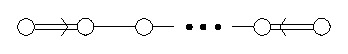
\includegraphics{table1_3(l)} & \includegraphics{table1_3(r)}
  \\ \hline
$D_n$ & 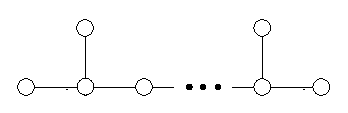
\includegraphics{table1_4(l)} & 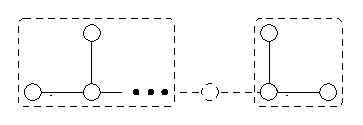
\includegraphics{table1_4(r)}
  \\ \hline
\end{tabular}
}
\caption{Подалгебры $\af,\;\afb$ для классических серий}
\end{table}

В случае серии $B$ ситуация отличается. Причина в том, что в данном случае подалгебра $\afb$ может быть больше, чем результат удаления поддиаграммы  $\af$ и соседних вершин. Подалгебры ортогональной пары $\ \af$ и $\afb$ не обязаны образовывать прямую сумму в $\gf$. Можно явно проверить, что при  $\gf=B_{r}$ и $\af=B_{r_{\af}}$ ортогональная подалгебра -- это $\afb=B_{r-r_{\af}}$. Рассмотрим вложение $B_{r_{\af}}\rightarrow B_{r},\quad 1<r_{\af}<r$. В результате удаления простого корня  $\alpha _{r_{\af}-1}=e_{r_{\af}-1}-e_{r_{\af}}$ расширенная диаграмма Дынкина для $B_{r}$ разбивается на несвязные диаграммы $\af=B_{r_{\af}}$ и $D_{r-r_{\af}}$. Однако корневая система  $\Delta _{\afb}$ содержит не только простые корни  $\left\{ e_{1}-e_{2},e_{2}-e_{3},\ldots ,e_{r_{\af}-2}-e_{r_{\af}-1},e_{1}+e_{2}\right\} $, но и корень $e_{r_{\af}-1}$. То есть  $\Delta _{\afb}$ образует систему типа  $B_{r-r_{\af}}$ и ортогональная пара для вложения $B_{r_{\af}}\rightarrow B_{r}$ -- это  $\left( B_{r_{\af}},B_{r-r_{\af}}\right) $. В следующем разделе мы приводим пример такой ортогональной пары для вложения $B_{2}\rightarrow B_{4}$ (см. Рис. \ref{fig:dynkin}).

Полная классификация регулярных подалгебр аффинных алгебр Ли приведена в недавней работе \cite{1751-8121-41-36-365204}. Из полной классификации максимальных специальных подалгебр классических алгебр Ли \cite{dynkin1952semisimple} мы получаем следующий список пар ортогональных подалгебр $\af,\;\afb$:
\begin{equation*}
\begin{array}{lll}
su(p)\oplus su(q) & \subset su(pq) &  \\
so(p)\oplus so(q) & \subset so(pq) &  \\
sp(2p)\oplus sp(2q) & \subset so(4pq) &  \\
sp(2p)\oplus so(q) & \subset sp(2pq) &  \\
so(p)\oplus so(q) & \subset so(p+q) & \text{для нечетных}\;p\;\text{и}\;q.
\end{array}
\end{equation*}


\subsubsection{Алгоритм рекурсивного вычисления коэффициентов ветвления}

\label{sec:algorithm}

Рекуррентные соотношения (\ref{recurrent-relation}) позволяют нам сформулировать алгоритм для рекурсивного вычисления коэффициентов ветвления. При этом для работы алгоритма не требуется построение модуля $L^{(\mu)}_{\gf}$ или какого-то из модулей $L^{(\nu)}_{\af}$

Алгоритм состоит из следующих шагов:

\begin{enumerate}[(i)]
\item Построить корневую систему $\Delta _{\af}$ для вложения $\af\rightarrow \gf$.

\item Выбрать все положительные корни $\alpha \in \Delta ^{+}$, ортогональные к  $\af$, то есть сформировать множество $\Delta_{\afb }^{+}$.

\item Построить множество $\Gamma _{\af\rightarrow \gf}$. Соотношение  (\ref{eq:142}) определяет знаковую функцию $s(\gamma)$ и множество $\Phi_{\af\subset \gf}$. Вычитание наименьшего веса $\gamma_0$ дает веер вложения (\ref{fan-defined}):
 $\Gamma _{\af\rightarrow \gf}=\left\{ \xi -\gamma _{0}|\xi \in \Phi _{\af\subset \gf}\right\} \setminus \left\{ 0\right\}$.

\item Построить множество $\widehat{\Psi ^{(\mu )}}=\left\{ w (\mu +\rho
)-\rho ;\;w \in W\right\} $ сингулярных весов для  $\gf$-модуля $L^{(\mu )}$.

\item Выбрать веса $\left\{ \mu _{\widetilde{\afb}}\left( w\right) =\pi _{\widetilde{\afb}}\left[ w(\mu +\rho
)-\rho \right] -\mathcal{D}_{\afb}\in \overline{C_{\widetilde{\afb}}}\right\} $. Так как множество  $\Delta_{\afb }^{+}$ фиксировано, легко осуществить проверку принадлежности веса $\mu _{\widetilde{\afb}}\left( w\right) $ к главной камере Вейля $\overline{C_{\widetilde{\afb}}}$ (достаточно вычислить скалярные произведения с фундаментальными весами $\afb^{+}$).

\item Для весов $\mu _{\widetilde{\afb}}\left( w\right) $ вычислить размерности соответствующих модулей, $\mathrm{\dim }\left(L_{\widetilde{\afb}}^{\mu _{\widetilde{\afb}}\left( u\right) }\right) $, используя формулу Вейля для размерностей. Затем построить сингулярный элемент $\Psi ^{\left( \mu \right) }_{\left(  \af, \afb \right)}$.

\item Вычислить сингулярные коэффициенты ветвления используя рекуррентное соотношение (\ref{recurrent-relation}) и выбрать среди них те, которые соответствуют весам в главной камере Вейля $\overline{C_{\af}}$.
\end{enumerate}

Можно ускорить работу алгоритма путем однократного вычисления представителей классов смежности $W/W_{\afb }$.

Следующий раздел состоит из примеров, иллюстрирующих применение данного алгоритма.

\section{Примеры}
\label{sec:branching-examples}

\subsection{Ветвления модулей конечномерных алгебр Ли}
\label{sec:finite-dimens-lie}

\subsubsection{Регулярное вложение $A_1$ в $B_2$}
\label{sec:regul-embedd-a_1}

Рассмотрим регулярное вложение $A_1\to B_2$. Простые корни $\alpha_1, \alpha_2$ алгебры $B_2$ обозначены пунктирными стрелками на Рисунке \ref{fig:B2_A1}. Мы обозначаем соответствующие элементарные отражения через $w_1, w_2$. Простой корень $\beta = \alpha_1+2\alpha_2$ алгебры $A_1$ показан серым цветом.


\begin{figure}[p]
  \noindent\centering{
    \includegraphics[width=80mm]{figure1}
  }
  \caption{Регулярное вложение  $A_1$ в $B_2$. Простые корни  $\alpha_1, \alpha_2$ алгебры $B_2$ обозначены пунктирными стрелками. Простой корень $\beta = \alpha_1+2\alpha_2$ подалгебры $A_1$ показан серым цветом. Старший вес фундаментального представления $L^{(1,0)=\omega_1}_{B_2}$ выделен черным. Веса сингулярного элемента $\Psi^{(\omega_1)}$ отмечены кругами с подписанными значениями соответствующих определителей $\epsilon(w)$.}
  \label{fig:B2_A1}

%\end{figure}
%\begin{figure}[pb]
  \noindent\centering{
    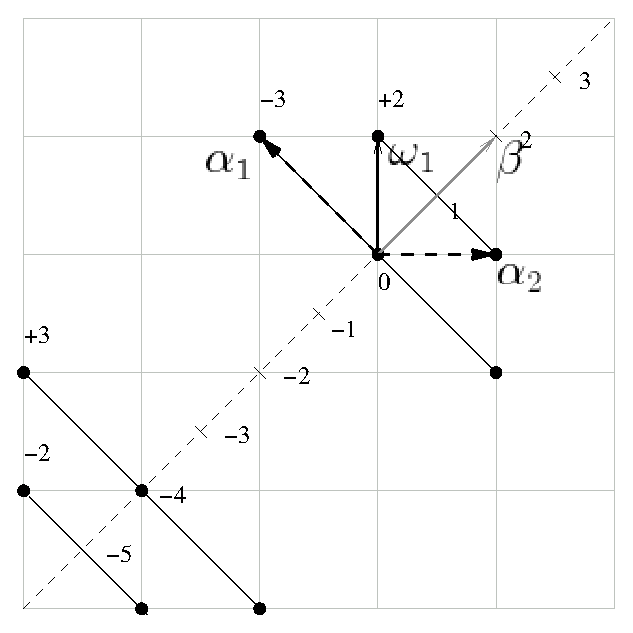
\includegraphics[width=80mm]{figure2}
  }
  \caption{Здесь диаграмма, показанная выше (Рисунок \ref{fig:B2_A1}), дополнена весами $\left( \afb=A_1 \right)$-модулей $L_{\af_{\perp }}^{\mu_{\af_{\perp }}\left( u\right) }$, построенных в точках $\pi _{\af}\left[ u(\mu +\rho )-\rho \right] $ и показанных пунктирными линиями. 
    Подписи к старшим весам   $\mu_{\af_{\perp }}\left( u\right)$ представляют собой значения произведений $\epsilon(u)\dim\left(L_{\afb}^{\mu_{\af_{\perp }}\left( u\right) }\right)$.
    Координаты вдоль корня $\beta$ указаны по отношению к фундаментальному весу $\af$. }
\label{fig:B2_A1_2}
\end{figure}

Выполним редукцию фундаментального представления  $L^{(1,0)=\omega_1}_{B_2}$ ($\omega_1$ -- черная стрелка на Рисунке \ref{fig:B2_A1}) в соответствии с алгоритмом.
Корень $\alpha_1$ ортогонален к $\beta$, так что  $\Delta_{\afb}^+ = \left\{ \alpha_1 \right\}$ (шаг (ii)).
В соответствии с Определением \ref{fan-definition} веер вложения $\Gamma_{A_1\to B_2}$ (шаг (iii)) состоит из двух весов:
\begin{equation*}
  \label{eq:22}
  \Gamma_{A_1\to B_2}=\left\{ (1;2),\; (2;-1) \right\},
\end{equation*}
где вторая компонента -- это значение знаковой функции  $s(\gamma)$.
Сингулярные веса  $\left\{ w (\omega_1 +\rho)-\rho ;\;w \in W\right\}$ (шаг (iv)) показаны кругами с подписанными значениями $\epsilon\left( w \right)$. Пространство  $U$ представляет собой факторпространство $W/W_{\afb}$, где $W_{\afb}=\left\{e,w_1\right\}$. Это означает, что сингулярные веса, находящиеся над прямой, заданной корнем $\beta$, принадлежат главной камере Вейля $\overline{C_{\widetilde{\af_{\perp }}}}$. Из формулы (\ref{defect-perp})  мы получаем  $\mathcal{D}_{\af_{\perp }}=0$ и $\hf_{\perp }=0$, то есть $\left\{ \mu _{\afb}\left( w\right)=\pi _{\afb}\left[ w(\mu +\rho)-\rho \right]\right\}$. Значит есть четыре старших веса для $\af_{\perp }$-модулей.  В базисе фундаментального веса $\frac{1}{2} \alpha_1$ алгебры $\afb$ координаты этих весов
$\left\{ \mu _{\afb}\left( u\right)=\pi _{\afb}\left[ u(\mu +\rho)-\rho \right]| u \in U \right\}$
равны
$\left\{ \left( 1\right) \left( 2\right) \left( 2\right) \left( 1\right) \right\}$ (шаг v).
На Рисунке (\ref{fig:B2_A1_2}) соответствующие весовые диаграммы
$\left\{ \mathcal{N}_{\af_{\perp }}^{\mu _{\af_{\perp }}\left( u\right) }\right\} $
построены из весов $\left\{ \mu _{\af}\left( u\right)\right\} =\left\{\pi _{\af}\left[ u(\mu +\rho )-\rho \right]\right\}
=\left\{ \left( 1\right) \left( 0\right) \left( -4\right) \left( -5\right) \right\}$ подалгебры   $\af$.
В действительности весовые диаграммы нам не нужны, достаточно знать лишь размерности модулей
$L_{\af_{\perp }}^{\mu_{\af_{\perp }}\left( u\right) }$ умноженные на
$\epsilon \left( u\right) $ (шаг vi). Полученные значения должны быть связаны с точками
$\left\{ \left( 1\right) \left( 0\right) \left( -4\right) \left( -5\right) \right\}$ в $P_{\af}$. Сингулярный элемент $\Psi ^{\left( \mu \right) }_{\left(  \af, \afb \right)}$ содержит следующий набор весов и их сингулярных кратностей:
\begin{equation}
  \label{eq:25}
  \left\{(1;2),\; (0;-3),\; (-4;3),\; (-5;-2)\right\}.
\end{equation}

Применяя формулу (\ref{recurrent-relation}) с веером
$\Gamma_{A_1\to B_2}$ к множеству (\ref{eq:25}) (шаг vii)
мы получаем нули для весов больше старшего сингулярного вектора$(1;2)$ и  $k^{(1,0)}_1=2$ для самого вектора $(1;2)$.
Для сингулярного веса $(0;-3)$ на границе $\bar{C}^{(0)}_{\af}$ рекуррентное соотношение дает
\begin{equation*}
  \label{eq:23}
  k^{(1,0)}_{0}=-1\cdot k^{(1,0)}_2 +2\cdot k^{(1,0)}_1 - 3\cdot \delta_{0,0} = 1,
\end{equation*}
и редукция завершена: $L_{B_2\downarrow A_1}^{\omega_1}=
2L_{A_1}^{\omega_{\left(A_1\right)} }
\bigoplus
L_{A_1}^{2\omega_{\left(A_1\right)} }$.

\subsubsection{Вложение  $B_2$ в $B_4$}
\label{sec:someth-high-dimens}
Рассмотрим регулярное вложение $B_2 \rightarrow B_4$. Соответствующие диаграммы Дынкина показаны на Рисунке \ref{fig:dynkin}.
\begin{figure}[h]
  \centering
  \includegraphics[width=60mm]{figure3}
  \caption{Регулярное вложение  $B_2 \rightarrow B_4$ получается путем исключения вершины из диаграммы Дынкина. 
    Напомним, что в данном случае $\afb$ равна $B_2$, тогда как на диаграмме видна только подалгебра $A_1\oplus A_1$ (см. раздел \ref{sect-embeddings}).}
  \label{fig:dynkin}
\end{figure}

\begin{figure}[pt]
  \centering
    \includegraphics[width=100mm,height=90mm]{figure4}
  \caption{Сингулярный элемент  $e^{\gamma_0}\Psi ^{\left( \mu \right) }_{\left(  \af, \afb \right)}$ показан в весовом подпространстве $P_{\af}$, где $\af=B_2$ и базис равен $\left\{e_3,e_4\right\}$. Показаны спроектированные сингулярные веса $\left\{\pi _{\af}\left[ u(\mu +\rho )-\rho \right] +\gamma_0 | u \in U \right\}$, сдвинутые на  $\gamma_0$ и снабженные множителям  $\epsilon(u)\dim\left(L_{\af_{\perp }}^{\mu_{\af_{\perp }}\left( u\right) }\right)$.}
  \label{fig:B4B2anom}

%\end{figure}
%
%\begin{figure}[pb]
  \centering
  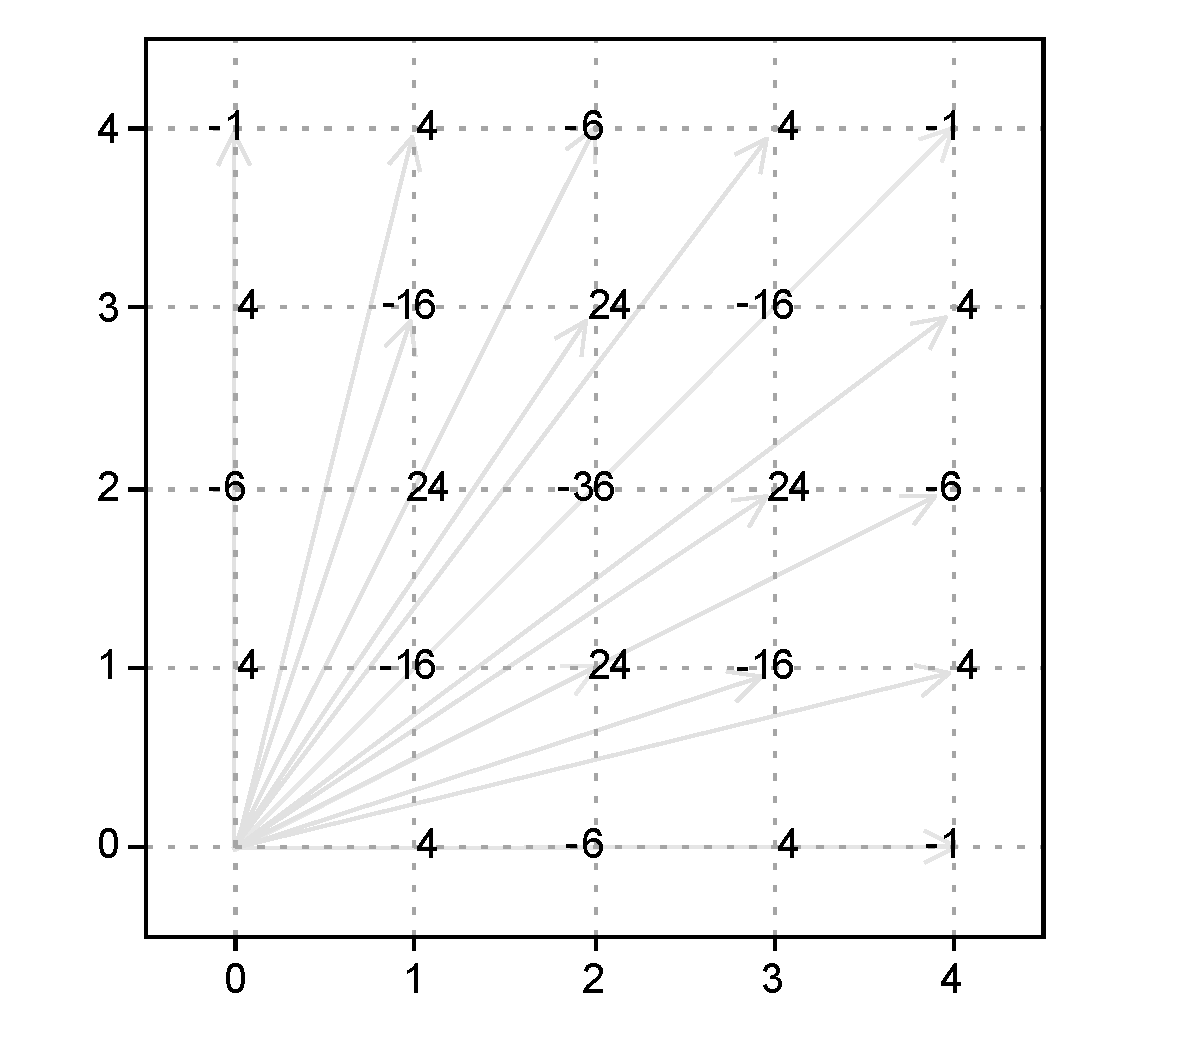
\includegraphics[height=80mm]{figure5}
  \caption{Веер $\Gamma$ для вложения $B_2\rightarrow B_4$ со значениями функции $s(\gamma+\gamma_0)$, указанными при соответствующих весах $\gamma \in \Gamma$.}
  \label{fig:B4B2Fan}
\end{figure}

В ортогональном базисе $\left\{e_1,\dots,e_4\right\}$ простые и положительные корни алгебры $B_4$ равны
\begin{eqnarray*}
  \label{eq:19}
  S_{B_4}= \{e_1 - e_2,\; e_2 - e_3,\; e_3 - e_4,\; e_4\},\\[2mm]
 \Delta^+_{B_4}=\left\{ (e_1 - e_2,\; e_2 - e_3,\; e_3 - e_4,\; e_4,\; e_1 - e_3,\; e_2 - e_4,\; e_3 + e_4,\; e_3,\; e_1 - e_4,\;\right.\\
 \left. e_2 + e_4,\; e_2,\; e_1 + e_4,\; e_2 + e_3,\; e_1,\; e_1 + e_3,\; e_1 + e_2\right\}
\end{eqnarray*}
Подалгебра  $\af=B_2$ задается простыми корнями
\begin{equation*}
  \label{eq:155}
 S_{B_2}=\{e_3-e_4,e_4\}.
\end{equation*}
Ее ортогональный партнер $\afb=B_2$ определяется корнями
\begin{eqnarray*}
  \label{eq:27}
  S_{\afb}=\{e_1-e_2,e_2\},\\
 \Delta^{+}_{\afb}= \left\{e_1-e_2,e_1+e_2,e_1,e_2\right\}.
\end{eqnarray*}
После определения множества $\Delta^+_{B_4} \setminus  \Delta^{+}_{\afb}$ можно построить веер вложения $\Gamma_{B_2 \to B_4}$ применяя Определение \ref{fan-definition}. Так как для этого вложения $s\left( \gamma_0\right)=-1$, в рекуррентном соотношении нам нужен только множитель $s\left(\gamma + \gamma_0\right)$. Результат построения веера показан на Рисунке \ref{fig:B4B2Fan}.

Рассмотрим модуль $L^{\mu}$ алгебры  $B_4$ со старшим весом $\mu=2e_1 + 2 e_2 + e_3 + e_4$; \,
$\mathrm{dim}(L^{\left[0,1,0,2\right]})=2772$.
В данном случае дефект не равен нулю, $\mathcal{D}_{\af_{\perp }}=-2\left( e_1 + e_2 \right)$, тогда как $\hf_{\bot}$ тривиальна. Среди сингулярных весов есть 
48 векторов со свойством $\left\{ \mu _{\afb}\left( u\right) =\pi _{\af_{\perp }}\left[ u(\mu +\rho)-\rho \right] -\mathcal{D}_{\afb}\in \overline{C_{\afb}}\right\} $.
Таким образом мы определили множество $U=\left\{ u \right\}$. Вычислим размерности соответствующих  $\afb$-модулей со старшими весами $\mu_{\afb}\left( u\right)$ (используем формулу Вейля для размерностей) и умножим их на $\epsilon\left( u \right)$. В результате получим сингулярный элемент
$\Psi ^{\left( \mu \right) }_{\left(  \af, \afb \right)}$, показанный на Рисунке \ref{fig:B4B2anom}.

Теперь поместим веер  $\Gamma$ (см. Рисунок \ref{fig:B4B2Fan}) в старший из весов, показанных на Рисунке \ref{fig:B4B2anom} и проведем рекурсивное вычисление коэффициентов ветвления (с использованием соотношения (\ref{recurrent-relation})):
\begin{eqnarray*}
  \label{eq:24}
  \pi_{\af} \left(ch L^{\left[0,1,0,2\right]}_{B_4}\right) = 6 \; ch L^{\left[0,0\right]}_{B_2}+ 60
  \; ch L_{B_2}^{\left[0,2\right]}+ 30 \; ch L_{B_2}^{\left[1,0\right]}+ 19 \; ch L_{B_2}^{\left[2,0\right]}+\\
  40 \; ch L_{B_2}^{\left[1,2\right]}+ 10 \; ch L_{B_2}^{\left[0,4\right]}.
\end{eqnarray*}
%\newpage
\subsection{Примеры приложений в конформной теории поля}
\label{sec:phys-appl}

\subsubsection{Конформные вложения}
\label{sec:conformal-embeddings}

Как мы уже объясняли в разделе \ref{sec:modular-invariance}, коэффициенты ветвления для вложения аффинной алгебры Ли в аффинную алгебру Ли можно использовать для построения модулярно-инвариантной статсуммы для моделей Весса-Зумино-Новикова-Виттена в двумерной конформной теории поля (\cite{difrancesco1997cft}, \cite{Walton:1999xc}, \cite{walton1989conformal}, \cite{schellekens1986conformal}).
В этих моделях аффинные алгебры Ли являются алгебрами токов. 

Модулярная инвариантность статсуммы необходима для самосогласованности теории на торе и римановых поверхностях высшего рода, что важно для приложений конформной теории поля в теории струн и описании критического поведения.

Простейшая модулярно-инвариантная статсумма имеет диагональный вид:
\begin{equation}
  \label{eq:148}
   Z(\tau)=\sum_{ \mu\in P^{+}_{\mathfrak{g}}} \chi_{\mu}(\tau)\bar \chi_{\mu}(\bar \tau)
\end{equation}
Здесь суммирование ведется по множеству старших весов интегрируемых модулей в ВЗНВ-модели, а $\chi_{\mu}(\tau)$ -- это нормированные характеры (см. \cite{difrancesco1997cft}) этих модулей.

Построение недиагональных модулярных инвариантов -- это нетривиальная проблема, хотя для некоторых моделей известна полная классификация модулярных инвариантов \cite{1994hepthGannon,1995JMPGannon}.

Рассмотрим модель Весса-Зумино-Новикова-Виттена с аффинной алгеброй Ли $\af$. Недиагональные модулярные инварианты этой модели могут быть построены из диагонального инварианта, если существует аффинная алгебра  $\mathfrak{g}$, такая, что $\af\subset\mathfrak{g}$. Тогда мы можем заменить характеры  $\mathfrak{g}$-модулей в диагональной модулярно-инвариантной статсумме (\ref{eq:148}) на разложения
\begin{equation*}
  \label{eq:32}
\sum_{\nu \in P^{+}_{\af}}b^{(\mu)}_{\nu} \chi_{\nu},
\end{equation*}
содержащие нормированные характеры $\chi_{\nu}$ соответствующих $\af$-модулей. В результате мы получим недиагональную модулярно-инвариантную статсумму для теории с алгеброй токов $\af$,
\begin{equation}
  \label{eq:154}
   Z_{\af}(\tau)=\sum_{ \nu,\lambda\in P^{+}_{\af}} \chi_{\nu}(\tau)M_{\nu\lambda}\bar \chi_{\lambda}(\bar \tau).
\end{equation}

Эффективная процедура редукции существенна для этой конструкции. Вложение должно сохранять конформную инвариантность. Пусть $J^{\alpha_j}_{-n_j}$ и $\tilde{J}^{\alpha'_j}_{-n_j}$ -- понижающие операторы для алгебры $\mathfrak{g}$ и подалгебры $\af\subset\mathfrak{g}$ соответственно. Обозначим через $\pi_{\af}$ оператор проекции $\pi_{\af}:\mathfrak{g}\longrightarrow \af$. В теории, связанной с $\mathfrak{g}$ и вакуумом $\left|\lambda\right>$ состояния строятся как
\begin{equation*}
  \label{eq:151}
  J^{\alpha_1}_{-n_1}J^{\alpha_2}_{-n_2}\dots\left|\lambda\right>\quad n_1\geq n_2\geq \dots>0.
\end{equation*}
А для подалгебры $\af$ соответствующие состояния имеют вид
\begin{equation*}
  \label{eq:152}
  \tilde{J}^{\alpha'_1}_{-n_1}\tilde{J}^{\alpha'_2}_{-n_2}\dots\left|\pi_{\af}(\lambda)\right>.
\end{equation*}
Инвариантность вакуума под действием $\mathfrak{g}$ влечет его инвариантность относительно действия $\af$, но это неверно для тензора энергии-импульса. Необходимо, чтобы тензор энергии-импульса объемлющей теории содержал только генераторы $\tilde{J}$. Тогда соотношение
\begin{equation}
  \label{eq:127}
  T_{\mathfrak{g}}(z)=T_{\af}(z)
\end{equation}
ведет к равенству центральных зарядов
\begin{equation*}
  \label{eq:33}
  c(\mathfrak{g})=c(\af)
\end{equation*}
и к уравнению
\begin{equation}
  \label{eq:153}
  \frac{k\;\mathrm{dim}\,\mathfrak{g}}{k+h^{\vee}_{\gf}}=\frac{x_e k\; \mathrm{dim}\,\af}{x_ek+h^{\vee}_{\af}}.
\end{equation}
Здесь $x_e$ -- так называемый ``индекс вложения'':
$x_e=\frac{\left|\pi_{\mathfrak{a}} \theta\right|^2}{\left|\theta_{\mathfrak{a}}\right|^2}$, где $\theta$, $\theta_{\mathfrak{a}}$ -- старшие корни алгебр
$\mathfrak{g}$ и $\mathfrak{a}$, а  $h^{\vee}_{\gf}$ и $h^{\vee}_{\af}$ -- дуальные числа Кокстера.

Можно показать, что решения уравнения (\ref{eq:153}) существуют только для уровня $k=1$ \cite{difrancesco1997cft}.

Полная классификация конформных вложения дана в работе \cite{schellekens1986conformal}.

Если рассмотреть соотношение (\ref{eq:153}) и асимптотику функций ветвления, то можно доказать теорему о конечной приводимости \cite{kac1988modular}. Она утверждает, что для конформного вложения  $\af\longrightarrow\mathfrak{g}$ лишь конечное число коэффициентов ветвления отлично от нуля.

\begin{mynote} Ортогональная подалгебра  $\afb$ всегда тривиальна в случае конформного вложения $\af\longrightarrow \mathfrak{g}$.
\begin{proof}
Рассмотрим разложение тензора энергии-импульса на моды:
\begin{equation*}
\label{eq:47}
  T(z)=\frac{1}{2(k+h^v)}\sum_n z^{-n-1}L_n.
\end{equation*}
Моды $L_n$ представляют собой комбинации нормально упорядоченных произведений генераторов алгебры $\gf$,
\begin{equation*}
\label{eq:48}
  L_n=\frac{1}{2(k+h^v)}\sum_{\alpha}\sum_m:J^{\alpha}_m J^{\alpha}_{n-m}: \; .
\end{equation*}
При конформном вложении тензоры энергии-импульса  $T_{\mathfrak{g}}(z)$ и $T_{\af}(z)$ равны (см. (\ref{eq:127})).

В эти комбинации мы должны подставить генераторы подалгебры $\af$ выраженные через генераторы $\mathfrak{g}$ и получить тензор энергии-импульса $T_{\mathfrak{g}}$. Но если набор генераторов, связанных с  $\Delta_{\afb}$ не пуст, это не возможно, так как  $T_{\mathfrak{g}}$ содержит генераторы $J^{\alpha}_n$, где $\alpha\in \Delta_{\afb}$.
\end{proof}
\end{mynote}



\subsubsection{Специальное вложение $\hat{A}_1\rightarrow\hat{A}_2$.}
\label{sec:spec-embedd-hata_1s}
Рассмотрим следующие пример аффинной алгебры Ли $\gf$ и аффинной подалгебры $\af$:
$\hat{A}_1 \rightarrow \hat{A}_2$ и вложение является аффинным расширением специального вложения $A_1 \rightarrow A_2$ с индексом вложения $x_e=4$. Так как мы должны рассматривать $\gf$-модули уровня один, соответствующие  $\af$-модули будут иметь уровень $\tilde{k}=kx_e=4$.

Существует три фундаментальных веса алгебры  $\hat{A}_2$ имеющих уровень один. 
Легко видеть, что множество $\Delta_{ \afb }$ пусто и подалгебра $\afb=0$. Тогда ${\cal D}_{\afb}=0$, $\hf_{\perp}$ -- одномерная абелева подалгебра и размерность $\tilde\afb=\afb\oplus \hf_{\perp}$ также равна 1. Удобно выбрать классический корень для подалгебры $\hat{A}_1$ равным $\beta=\frac{1}{2}(\alpha_1+\alpha_2)$.

Используем Определение (\ref{fan-definition}) и построим веер $\Gamma_{\hat A_1\to\hat A_2}$. В этом случае $\gamma_0 =0$ и знак  $s\left( 0 \right)=-1$, то есть мы используем знаковую функцию $s(\gamma)$ (см. Рисунок \ref{fig:AffineA2A1Fan}).


\begin{figure}[h!bt]
  \centering
  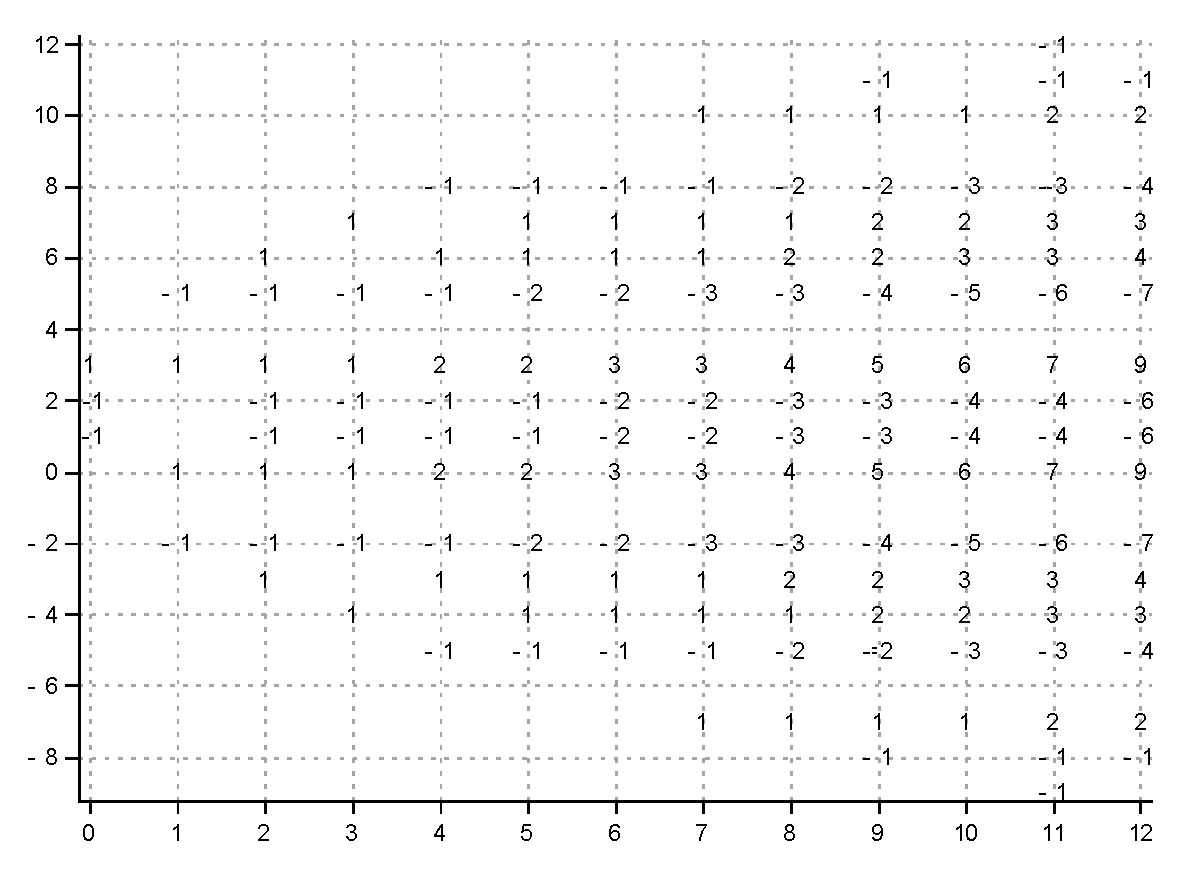
\includegraphics[width=125mm]{figure6}

  \caption{Веер  $\Gamma_{\hat{A_1}\rightarrow \hat{A_2}}$ для вложения $\hat{A_1}\rightarrow \hat{A_2}$ в базисе $\left\{\beta,\delta \right\}$. Заметим, что  $\gamma_0 =0$ и значения $s(\gamma)$ приписаны к весам $\gamma\in \Gamma_{\hat{A_1}\rightarrow \hat{A_2}}$}
  \label{fig:AffineA2A1Fan}
\end{figure}

Рассмотрим модуль $L^{\omega_0=(0,0;1;0)}$. Здесь мы используем обозначение (конечномерная часть; уровень; грейд)
для старшего веса и координаты конечномерной части даются индексами Дынкина (см. раздел \ref{sec:weights-roots}).

Множество весов $\widehat{\Psi^{(\omega_0)}}$ показано на Рисунке \ref{fig:affine_A2_anom_point} вплоть до шестого грейда.

\begin{figure}[h!tb]
  \hspace*{-1.5cm}
  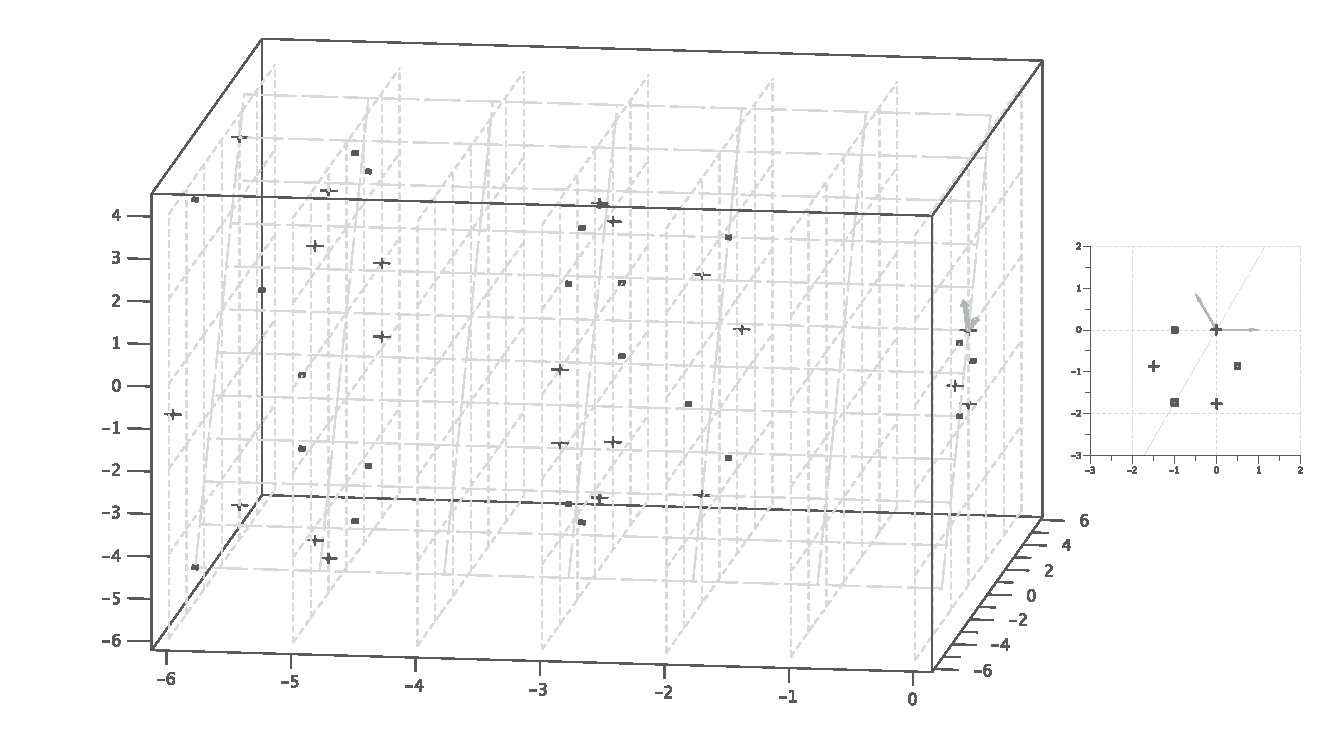
\includegraphics[width=180mm]{figure7}
  \caption{Сингулярные веса модуля $L_{\hat{A_2}}^{\omega_0}=L^{(0,0;1;0)}_{\hat{A_2}}$. Классическое сечение (нулевой грейд) диаграммы показано отдельно в правой части рисунка. 
    Мы используем ортогональный базис с единичным вектором, равным $\alpha_1$. Веса $w (\omega_0+\rho)-\rho$ показаны крестами, если $\epsilon(w)=1$ и квадратами при $\epsilon(w)=-1$. Простые корни классической подалгебры  $A_2$ показаны серым, а диагональная плоскость соответствует подалгебре Картана вложенной алгебры $\hat{A}_1$.}
  \label{fig:affine_A2_anom_point}
\end{figure}

Следующий шаг состоит в проектировании сингулярных весов на $P_{\hat A_1}$. В результате получается элемент $\Psi ^{\left( \omega_0 \right) }_{\left(  \hat A_1\, , \, \afb=0 \right)}$, изображенный на Рисунке \ref{fig:AffineA2_A1_anom_proj} вплоть до двенадцатого грейда.
\begin{figure}[h!tb]
  \centering
  \includegraphics[width=130mm]{figure8}
  \caption{Сингулярный элемент $\Psi ^{\left( \omega_0 \right) }_{\left(  \hat A_1\, , \, \afb=0 \right)}$ показан в $P_{\hat A_1}$ с базисом $\left\{\beta,\delta \right\}$.}
  \label{fig:AffineA2_A1_anom_proj}
\end{figure}

Используя рекуррентное соотношение  (\ref{recurrent-relation}) с веером
$\Gamma_{\hat{A_1}\rightarrow \hat{A_2}}$ и сингулярными весами $\Psi ^{\left( \omega_0 \right) }_{\left(  \hat A_1\, , \, \afb=0 \right)}$, мы получаем сингулярные коэффициенты ветвления, показанные на Рисунке \ref{fig:AffineA2_A1_branching}.
\begin{figure}[h!tb]
  \centering
  \includegraphics[width=130mm]{figure9}
  \caption{Сингулярные коэффициенты ветвления для вложения $\hat{A_1}\subset \hat{A_2}$. Границы главной камеры Вейля $\bar{C}_{\hat{A}_1}$ показаны черными линиями. Два сингулярных веса, расположенные в главной камере Вейля, отмечены звездочками. Они оба имеют кратность 1, то есть соответствующие коэффициенты ветвления равны 1.}
  \label{fig:AffineA2_A1_branching}
\end{figure}
Внутри камеры Вейля $\bar{C}_{\hat{A}_1}$ (ее границы показаны на Рисунке \ref{fig:AffineA2_A1_branching}) находятся только два ненулевых сингулярных веса и оба они имеют кратность 1. Это старшие веса подмодулей $\af$ и их кратности равны коэффициентам ветвления. То есть мы получаем разложение
\begin{equation*}
  \label{eq:43}
  L^{(0,0;1;0)}_{\hat{A_2}\downarrow \hat{A_1}}= L_{\hat{A_1}}^{(0;4;0)}\oplus L_{\hat{A_1}}^{(4;4;0)}.
\end{equation*}
Заметим, что теорема о конечной приводимости выполняется.

Тот же веер $\Gamma_{\hat{A_1}\rightarrow \hat{A_2}}$ можно использовать для других модулей старшего веса $L^{\mu}_{\hat{A_2}}$. В частности для неприводимых модулей уровня один мы получаем тривиальное ветвление:
\begin{eqnarray*}
  \label{eq:44}
   L^{(1,0;1;0)}_{\hat{A_2}\downarrow \hat{A_1}}= L_{\hat{A_1}}^{(2;4;0)},\\
   L^{(0,1;1;0)}_{\hat{A_2}\downarrow \hat{A_1}}= L_{\hat{A_1}}^{(2;4;0)}.
\end{eqnarray*}

Используя эти результаты легко получить модулярно-инвариантную статсумму:
\begin{equation*}
  \label{eq:45}
  Z=\left|\chi_{(4;4;0)}+\chi_{(0;4;0)}\right|^2+2\chi_{(2;4;0)}^2.
\end{equation*}

\subsubsection{Coset-модели}
\label{sec:coset-models}

Coset-модели \cite{Goddard198588}, тесно связанные с калибровочными ВЗНВ-моделями, активно изучаются в теории струн, особенно в струнных моделях в пространстве анти де Ситтера
\cite{Maldacena:2000hw,Maldacena:2000kv,Maldacena:2001km,Maldacena:2001ky,Aharony:1999ti}. Характеры в coset-моделях пропорциональны функциям ветвления.
\begin{equation}
  \label{eq:31}
  \chi^{(\mu)}_{\nu}(\tau)=e^{2\pi i \tau (m_{\mu}-m_{\nu})} b^{(\mu)}_{\nu}(\tau),
\end{equation}
где
\begin{equation*}
  \label{eq:46}
  m_{\mu}=\frac{\left|\mu+\rho\right|^2}{2(k+g)}-\frac{\left|\rho\right|^2}{2g}.
\end{equation*}
Проблема построения функций ветвления для  coset-моделей рассматривалась в работах  \cite{Dunbar:1992gh}, \cite{Hwang:1994yr}, \cite{lu1994branching}.

Вернемся к нашему примеру \ref{sec:regul-embedd-a_1} и рассмотрим аффинное расширение вложения $A_1 \rightarrow B_2$. Так как вложение регулярно и индекс $x_e=1$, модули подалгебры и исходный модуль имеют одинаковый уровень. Множество положительных корней с нулевой проекцией на корневое пространство подалгебры  $\hat{A_1}$ то же, что и в конечномерном случае: $\Delta^{+}_{\afb}=\left\{ \alpha_1 \right\}$ и $\afb=A_1$. Легко видеть, что здесь $\hf_{\perp}$ тривиальна и  ${\cal D}_{\afb}=0$.

Используя Определение \ref{fan-definition} мы получаем веер вложения $\Gamma_{\hat{A_1} \longrightarrow  \hat{B_2} }$. Заметим, что наименьший вес веера $\gamma_0$ равен нулю и  $s\left( \gamma_0 \right)=-1$. Значения знаковой функции  $s(\gamma)$ для $ \gamma \in \Gamma_{\hat{A_1} \longrightarrow  \hat{B_2} }$ показаны на Рисунке \ref{fig:AffineB2A1Fan}.
Мы ограничили вычисление двенадцатым грейдом. 
\begin{figure}[h!bt]
  \centering
  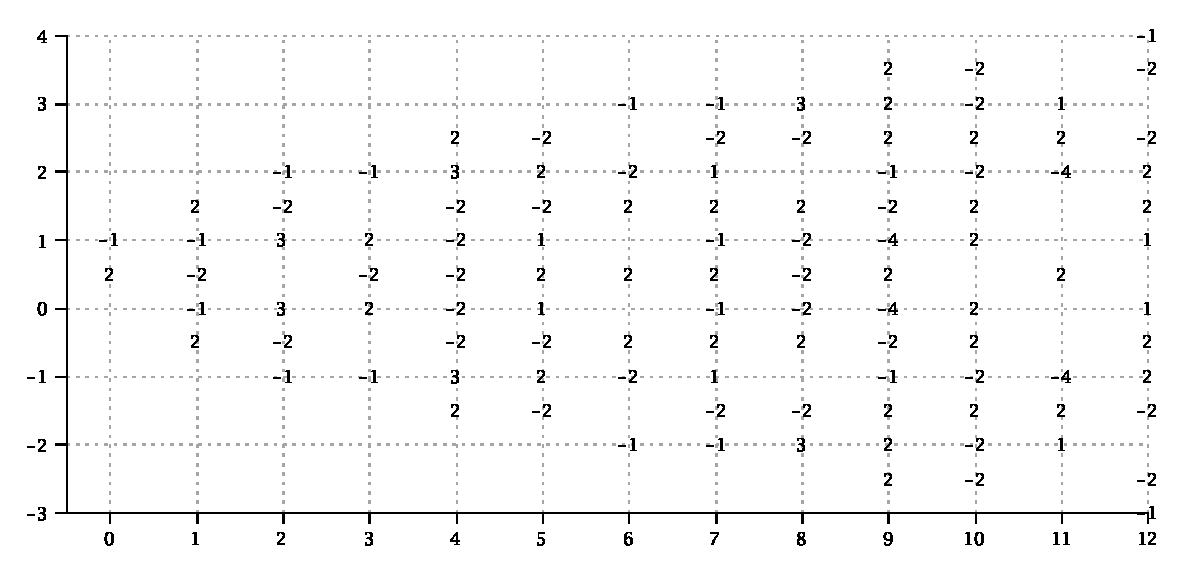
\includegraphics[width=135mm]{figure10}
  \caption{Веер $\Gamma_{\hat{A_1}\rightarrow \hat{B_2}}$ для вложения $\hat{A_1}\rightarrow \hat{B_2}$ в базисе $\left\{\beta,\delta \right\}$. Значения $s(\gamma)$ показаны для весов $\gamma\in \Gamma_{\hat{A_1}\rightarrow \hat{B_2}}$}
  \label{fig:AffineB2A1Fan}
\end{figure}

Рассмотрим модуль уровня один $L^{\left( 1,0;1;0 \right)}_{\hat{B_2}}$  со старшим весом  $\omega_1=(1,0;1;0)$, где координаты конечномерной части даны в ортогональном базисе $e_1,e_2$. Множество сингулярных весов для этого модуля вплоть до шестого грейда приведено на Рисунке \ref{fig:affine_B2_anom_point}.

\begin{figure}[h!tb]
%  \hspace*{-2cm}
  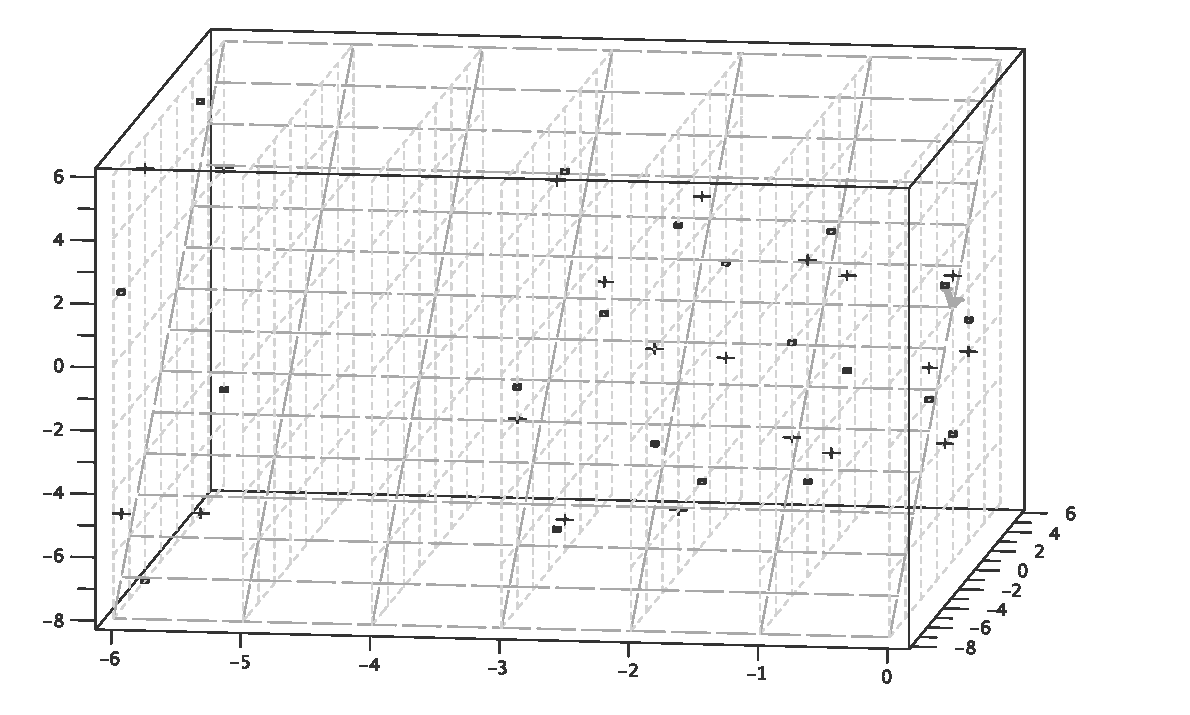
\includegraphics[width=140mm]{figure11}
  \caption{Сингулярные веса модуля $L^{(1,0;1;0)}_{\hat B_2 }$. В классическом сечении используется стандартный базис  $\{e_1,e_2\}$. Веса в нулевом грейде те же, что и на Рисунке \ref{fig:B2_A1}. Веса  $w (\omega_1+\rho)-\rho$ отмечены крестами, если $\epsilon(w)=1$ и квадратами при $\epsilon(w)=-1$. Простые корни классической подалгебры  $B_2$ показаны серым, а диагональная плоскость соответствует подалгебре Картана вложенной алгебры $\hat{A}_1$.}
  \label{fig:affine_B2_anom_point}
\end{figure}

В соответствии с рекурсивным алгоритмом  \ref{sec:algorithm} мы проектируем сингулярные веса на $P_{\hat{A_1}}$ и вычисляем размерности $\afb$-модулей $L^{\pi_{\afb}(w(\mu+\rho))-\rho_{\afb}}_{\afb}$. В нулевом грейде эта проекция дает в точности множество $\Psi ^{\left( \mu \right) }_{\left(  A_1, A_1 \right)}$, соответствующее вложению классической алгебры Ли  $A_1\rightarrow B_2$. Это можно заметить сравнивая Рисунок \ref{fig:B2_A1} и Рисунок \ref{fig:AffineB2_A1_anom_proj}, на котором сингулярный элемент $\Psi ^{\left( \mu \right) }_{\left(  \widehat{A_1}, A_1 \right)}$ для аффинного вложения  $\hat{A_1}\to\hat{B_{2}}$  показан вплоть до двенадцатого грейда. Кратности старших весов внутри главной камеры Вейля
$\bar{C}^{\left( 0 \right)}_{\hat{A_1}}$ определяют следующие значения коэффициентов ветвления (до двенадцатого грейда):
\begin{eqnarray*}
  \label{eq:28}
  L^{\omega_1}_{\hat{B_2}\downarrow \hat{A_1}}
  &=&2 L_{\hat{A_1}}^{\omega_1}\oplus 1 L_{\hat{A_1}}^{\omega_0}\oplus 4 L_{\hat{A_1}}^{\omega_0-\delta}\oplus\\
    &&2 L_{\hat{A_1}}^{\omega_1-\delta}\oplus 8 L_{\hat{A_1}}^{\omega_0-2\delta}\oplus
    8 L_{\hat{A_1}}^{\omega_1-2\delta}\oplus 15 L_{\hat{A_1}}^{\omega_0-3\delta}\oplus\\
    &&12 L_{\hat{A_1}}^{\omega_1-3\delta}\oplus 26 L_{\hat{A_1}}^{\omega_1-4\delta}\oplus
    29 L_{\hat{A_1}}^{\omega_0-4\delta}\oplus 51 L_{\hat{A_1}}^{\omega_0-5\delta}\oplus\\
    &&42 L_{\hat{A_1}}^{\omega_1-5\delta}\oplus 78 L_{\hat{A_1}}^{\omega_1-6\delta}\oplus
    85 L_{\hat{A_1}}^{\omega_0-6\delta}\oplus 120 L_{\hat{A_1}}^{\omega_1-7\delta}\oplus\\
    &&139 L_{\hat{A_1}}^{\omega_0-7\delta}\oplus 202 L_{\hat{A_1}}^{\omega_1-8\delta}\oplus
    222 L_{\hat{A_1}}^{\omega_0-8\delta}\oplus 306 L_{\hat{A_1}}^{\omega_1-9\delta}\oplus\\
    &&346 L_{\hat{A_1}}^{\omega_0-9\delta}\oplus 530 L_{\hat{A_1}}^{\omega_0-10\delta}\oplus
    482 L_{\hat{A_1}}^{\omega_1-10\delta}\oplus 714 L_{\hat{A_1}}^{\omega_1-11\delta}\oplus\\
    &&797 L_{\hat{A_1}}^{\omega_0-11\delta}\oplus 1080 L_{\hat{A_1}}^{\omega_1-12\delta}\oplus
    1180 L_{\hat{A_1}}^{\omega_0-12\delta}\oplus \dots
\end{eqnarray*}
\begin{figure}[h!tb]
  \centering
  \includegraphics[width=120mm]{figure12}
  \caption{Сингулярный элемент $\Psi ^{\left( \omega_1 \right) }_{\left(  \widehat{A_1}, A_1 \right)}$ в базисе $\{\beta,\delta\}$. Размерности соответствующих  $\afb=A_1$-модулей со знаками  $\epsilon(u)$ представлены на рисунке.}
  \label{fig:AffineB2_A1_anom_proj}
\end{figure}

\begin{figure}[tb]
  \centering
  \includegraphics[width=120mm]{figure13}
  \caption{Сингулярные коэффициенты ветвления для вложения $\hat{A_1}\rightarrow \hat{B_2}$. Использован базис $\{\beta,\delta\}$. Границы главной камеры Вейля $\bar{C}_{\hat{A}_1}$ показаны черными линиями. Сингулярные коэффициенты ветвления внутри главной камеры Вейля равны коэффициентам ветвления для вложения $\hat{A_1}\rightarrow \hat{B_2}$.}
  \label{fig:AffineB2_A1_branching}
\end{figure}

Этот результат можно представить в виде набора функций ветвления:
\begin{eqnarray*}
  \label{eq:29}
  \begin{array}{cc}
    b^{(\omega_1)}_{0}= & 1 + 4\,q^{1}+ 8\,q^{2}+ 15\,q^{3}+ 29\,q^{4}+ 51\,q^{5}+ 85\,q^{6}+ 139\,q^{7}+\\
     &222\,q^{8}+ 346\,q^{9}+ 530\,q^{10}+ 797\,q^{11}+ 1180\,q^{12}+\dots\\
  \end{array}\\
  \begin{array}{cc}
    b^{(\omega_1)}_{1}= &2+2\,q^{1}+8\,q^{2}+12\,q^{3}+26\,q^{4}+42\,q^{5}+78\,q^{6}+120\,q^{7}+\\
    & 202\,q^{8}+306\,q^{9}+482\,q^{10}+714\,q^{11}+1080\,q^{12}+\dots
  \end{array}
\end{eqnarray*}
Здесь $q=\exp (2\pi i \tau)$ и нижний индекс нумерует функции ветвления по их старшим весам в  $P^+_{\hat{A_1}}$, равным фундаментальным весам $\omega_0=\lambda_0=(0,1,0),\; \omega_1=\alpha/2=(1,1,0)$.

Теперь мы можем вернуться к равенству (\ref{eq:31}) и получить выражение для характеров coset-модели $B_2/A_1$:
\begin{equation*}
  \label{eq:35}
  \begin{array}{cc}
    \chi^{(\omega_1)}_{1}(q)= & q^{\frac{7}{12}}\left( 2+2\,q^{1}+8\,q^{2}+12\,q^{3}+26\,q^{4}+42\,q^{5}+78\,q^{6}+120\,q^{7}+\right. \\
    & \left. 202\,q^{8}+306\,q^{9}+482\,q^{10}+714\,q^{11}+1080\,q^{12}+\dots \right),\\
    \chi^{(\omega_1)}_{0}(q) = & q^{\frac{5}{6}}\left(1 + 4\,q^{1}+ 8\,q^{2}+ 15\,q^{3}+ 29\,q^{4}+ 51\,q^{5}+ 85\,q^{6}+ 139\,q^{7}+\right. \\
    &\left. 222\,q^{8}+ 346\,q^{9}+ 530\,q^{10}+ 797\,q^{11}+ 1180\,q^{12}+\dots\right).
  \end{array}
\end{equation*}

\section{Заключение}
\label{sec:conclusion}

Мы продемонстрировали, что техника веера вложения может использоваться для работы с произвольными редуктивными подалгебрами (как максимальными, так и не максимальными). Также показано, что проблема редукции для  $\af \subset \gf$ тесно связана со свойствами ортогонального партнера $ \afb $ подалгебры $\af$. Подалгебра  $\afb$ соответствует подмножеству положительных корней $\Delta^{+}_{\afb}$ в $\Delta_{\mathfrak{g}}^{+}$, которое тривиализует подалгебру Картана $\hf_{\afb}$. Веер вложения и множества сингулярных весов для модулей старшего веса алгебры $\gf$ существенным образом зависят от структуры  $\afb$ и ее подмодулей.  Для веера  $\Gamma_{\af\rightarrow \gf}$ эта зависимость почти очевидна: в элементе  $\Phi_{\af\rightarrow \gf}$ исключены множители, соответствующие корням  $\Delta^{+}_{\afb}$. Преобразование множества спроектированных сингулярных весов более интересно. Мы показали, что в новом сингулярном элементе $\Psi ^{\left( \mu \right) }_{\left(  \af, \afb \right)}$ коэффициенты зависят от $\afb$-подмодулей (их старшие веса $\mu _{\widetilde{\afb}}\left( u\right)$ заданы вложением и весами первоначального элемента $\Psi^{\mu}$). К счастью, для вычислений не требуется никакой информации о  $L^{\mu _{\widetilde{\afb}}\left( u\right)}_{\left\{ \afb \right\}}$-подмодулях, кроме их размерностей. В новом сингулярном элементе $\Psi ^{\left( \mu \right) }_{\left(  \af, \afb \right)}$ кратности весов равны размерностям $\dim\left(L^{\mu _{\widetilde{\afb}}\left( u\right)}_{\left\{ \afb \right\}}\right)$ соответствующих  $\afb$-модулей, умноженным на значения $\epsilon (u)$. В результате старшие веса подмодулей $\af$ и их кратности удовлетворяют набору линейных соотношений (\ref{eq:121}). Эти свойства выполняются для любой редуктивной подалгебры $\af\rightarrow \gf$ и уравнения могут быть переписаны в виде рекуррентных соотношений, которые можно решать последовательно.

Эффективность полученного алгоритма была продемонстрирована на различных примерах. В частности, мы рассмотрели построение модулярно-инвариантных статсумм в методе конформных вложений и coset-конструкцию моделей рациональной конформной теории поля. Эти конструкции полезны при изучении ВЗНВ-моделей, возникающих в контексте AdS/CFT соответствия \cite{Maldacena:2000hw,Maldacena:2000kv,Maldacena:2001km}.

Дальнейшее улучшение алгоритма может быть достигнуто при использовании техники сложенных вееров \cite{il2010folded}. Нужно отметить, что даже в случае струнных функций явное решение соответствующих рекуррентных соотношений представляет собой сложную проблему (см. подробности в работе\cite{il2010folded}). Тем не менее, мы надеемся, что развитие процедуры сложения позволит получить явные решения хотя бы для некоторых функций ветвления и соответствующих характеров coset-моделей.

%-----------------------------------------------------------------------------------------------------



%%
%% End of file
%%% Local Variables: 
%%% mode: latex
%%% TeX-master: "thesis"
%%% End: 


\chapter{Коэффициенты ветвления и обобщенная резольвента Бернштейна-Гельфанда-Гельфанда}
\label{cha:BGG}

Как мы показали в предыдущей главе, рекуррентные соотношения для коэффициентов ветвления основываются на определенном разложении сингулярного элемента. В данной главе мы показываем, что такое разложение может использоваться для построения параболических модулей Верма и получения обобщенных формул Вейля-Верма для характеров. Также мы демонстрируем, что ветвление для произвольной редуктивной подалгебры связано с БГГ резольвентой и демонстрирует свойства резольвенты в категории $\mathcal{O}^{p}$ \cite{lepowsky1977generalization} (параболического обобщения категории $\mathcal{O}$ \cite{bernstein1976category}).

Резольвента для неприводимых модулей в терминах бесконечномерных модулей важна для теории интегрируемых спиновых цепочек \cite{derk1008}. В подходе  $\mathcal{Q}$-оператора Бакстера \cite{derk09} общие трансфер-матрицы, соответствующие (обобщенным) модулям Верма, факторизуются в произведение операторов Бакстера. Резольвента позволяет вычислить трансфер-матрицы для конечномерных вспомогательных пространств.

Чтобы продемонстрировать связь БГГ резольвенты с ветвлением мы используем рекурсивный подход, представленный в работе \cite
{2010arXiv1007.0318L} (аналогичный подход для максимальных вложений использовался в работе \cite{ilyin812pbc}) и изложенный в главе \ref{cha:affine-lie-algebras}. Мы рассматриваем подалгебру $\af \hookrightarrow \gf$ вместе с $\afb$ -- ``ортогональным партнером'' $\af$ по отношению к форме Киллинга, а также подалгебру $\widetilde{\afb}:=\afb\oplus \frak{h}_{\perp }$, где $\frak{h}=\frak{\frak{h}_{\af}}\oplus
\frak{h}_{\afb}\oplus \frak{h}_{\perp }$. Для любой редуктивной подалгебры $\af$ алгебра $\afb\hookrightarrow \gf$ регулярна и редуктивна. Для интегрируемого модуля старшего веса $%
L^{\left(\mu \right) }$ и ортогональной подалгебры  $\af_{\bot }$ мы рассматриваем сингулярный элемент $\Psi ^{\left( \mu \right) }$ (числитель в формуле Вейля для характеров $ch\left( L^{\mu }\right) =\frac{\Psi ^{\left(
\mu \right) }}{\Psi ^{\left( 0\right) }}$, см. раздел \ref{sec:high-weight-modul}) и знаменатель Вейля $\Psi _{\af_{\bot
  }}^{\left( 0\right) }$ для ортогонального партнера. Ниже мы показываем, что элемент  $\Psi _{\gf%
}^{\left( \mu \right) }$ может быть разложен в комбинацию числителей Вейля $\Psi _{\af_{\bot }}^{\left( \nu \right) }$, где $\nu \in P_{%
\mathfrak{a}_{\bot}}^{+}$. Это разложение дает возможность построить множество модулей старшего веса $L_{\afb}%
^{\mu _{\afb}}$. В том случае, если вложение\ $\af%
_{\bot }\hookrightarrow \gf$ \ удовлетворяет ``стандартным параболическим'' условиям, эти модули порождают параболические модули Верма $M_{\left(
\afb \hookrightarrow \gf\right) }^{\mu _{%
\afb}}$, так что исходный характер $ch\left(
L^{\mu }\right) $ в итоге раскладывается в знакопеременную сумму таких модулей. С другой стороны, если параболическое условие нарушено, конструкция сохраняется и порождает разложение по отношению к набору обобщенных модулей Верма  $M_{\left( \widetilde{\frak{b}_{\perp }},\gf\right) }^{\mu _{%
\widetilde{\afb}}}$, где $%
\widetilde{\frak{b}_{\perp }}$ уже не является подалгеброй в $\gf$, а оказывается сжатием $\widetilde{\afb}$.

Возможные обобщения полученных результатов обсуждаются в Разделе \ref{sec:conclusions}.

\section{Ортогональная подалгебра и сингулярные элементы}

\label{sec:recurr-form-branch}

В этом разделе мы покажем, как рекуррентный подход к проблеме ветвления естественным образом приводит к представлению формального характера $\frak{g}$-модуля в виде комбинации характеров, соответствующих параболическим (обобщенным) модулям Верма. Рассмотрим редуктивную алгебру Ли  $\frak{g}$ и ее редуктивную подалгебру $\frak{a}\subset \frak{g}$.
Пусть  $L^{\mu} $ -- интегрируемый модуль старшего веса алгебры  $\frak{g}$, $\mu \in P^{+}$.  Будем считать  $L^{\mu}$ вполне приводимым по отношению к подалгебре $\frak{a}$,
\begin{equation*}
L_{\frak{g}\downarrow \frak{a}}^{\mu }=\bigoplus\limits_{\nu \in P_{\frak{a}%
}^{+}}b_{\nu }^{\left( \mu \right) }L_{\frak{a}}^{\nu }.
\end{equation*}
Это разложение может быть записано в терминах формальных характеров с использованием оператора проекции  $\pi _{\frak{a}}$ (на весовое пространство $\frak{h_{a}}^{\ast }$):
\begin{equation}
\pi _{\frak{a}}ch\left( L^{\mu }\right) =\sum_{\nu \in P_{\frak{a}%
}^{+}}b_{\nu }^{(\mu )}ch\left( L_{\frak{a}}^{\nu }\right) .
\label{branching12}
\end{equation}
Для модуля  $L^{\mu }$ существует БГГ резольвента (см. \cite
{bernstein1976category,bernstein1975differential,bernstein1971structure} и
\cite{humphreys2008representations}). Все члены фильтрующей последовательности представляются суммами модулей Верма со старшими весами $\nu$, сильно связанными с $\mu$:
\begin{equation*}
\left\{ \nu \right\} =\left\{ w\left( \mu +\rho \right) -\rho |w\in
W\right\} .
\end{equation*}

Воспользуемся введенным в главе \ref{cha:affine-lie-algebras} понятием ``ортогонального партнера''  $\mathfrak{a}_{\bot }\hookrightarrow \frak{g}$ для подалгебры   $\mathfrak{a}\hookrightarrow \frak{g}$.
Заметим, что подалгебра  $\mathfrak{a}_{\bot}$ по определению регулярна, так как она построена на подмножестве корней алгебры $\mathfrak{g}$.

\subsection{Разложение сингулярного элемента.}

\label{subsec:decomp-sing-element-again}

Выполним разложение сингулярного элемента  $\Psi ^{\left(\mu \right) }$ на сингулярные элементы модулей ортогонального партнера. Это разложение в целом аналогично разложению в Лемме \ref{lemma}, однако в данном случае его составляющими являются сингулярные элементы ортогонального партнера $\afb$.

\begin{lemma}

Пусть  $\frak{a}_{\bot }$ -- ортогональный партнер редуктивной подалгебры  $\frak{a}\hookrightarrow \frak{g}$ и $\frak{h}=\frak{\frak{h}_{\frak{a}}}\oplus \frak{h}_{\frak{a}_{\perp }}\oplus \frak{h}_{\perp }$, $\widetilde{%
\frak{a}_{\perp }}=\frak{a}_{\perp }\oplus \frak{h}_{\perp }$, $%
\widetilde{\frak{a}}=\frak{a}\oplus \frak{h}_{\perp }$.

Пусть $L^{\mu }$ -- интегрируемый модуль старшего веса  $\mu \in P^{+}$ и 

$\Psi ^{\left( \mu \right) }$\ -- сингулярный элемент $L^{\mu }$.

Тогда элемент  $\Psi ^{\left( \mu \right) }$ может быть разложен в сумму по  $u\in U$ (см. (\ref{U-def})) сингулярных элементов $\Psi _{\frak{a}_{\perp }}^{\mu _{\frak{a}_{\perp }}\left( u\right) }$ с коэффициентами
$\epsilon (u)e^{\mu _{\widetilde{\mathfrak{a}}}\left( u\right) }$:
\begin{equation}
\Psi ^{\left( \mu \right) }=\sum_{u\in U}\;\epsilon (u)e^{\mu _{\widetilde{%
\mathfrak{a}}}\left( u\right) }\Psi _{\frak{a}_{\perp }}^{\mu _{\frak{a}%
_{\perp }}\left( u\right) }.  \label{sing decomp main}
\end{equation}
\label{Psi-decomp-lemma}
\end{lemma}

\begin{proof}
Пусть
\[
u(\mu +\rho )=\pi _{\left( \aft\right) }u(\mu +\rho )+\pi _{\left(
\frak{a}_{\perp }\right) }u(\mu +\rho ),
\]
где $u\in U$. Для произвольного  $v\in W_{\frak{a}_{\bot }}$ рассмотрим сингулярный вес  $vu(\mu +\rho )-\rho $ и выполним разложение:
\begin{equation}
\begin{array}{lcl}
vu(\mu +\rho )-\rho  & = & \pi _{\left( \frak{a}\right) }\left( u(\mu +\rho
)\right) -\rho +\rho _{\frak{a}_{\perp }}
\\
&  & +\ v\left( \pi _{\left( \aft_{\perp }\right) }u(\mu
+\rho )-\rho _{\frak{a}_{\perp }}+\rho _{\frak{a}_{\perp }}\right) -\rho _{%
\frak{a}_{\perp }} .
\end{array}
\label{sing-decomp-2}
\end{equation}
Используем дефект $\mathcal{D}_{\frak{a}_{\bot }}$ (\ref{defect-perp}), чтобы упростить первую строку в формуле (\ref{sing-decomp-2}):
\[
\begin{array}{r}
\pi _{\left( \aft\right) }\left( u(\mu +\rho )\right) -\rho +\rho _{%
\frak{a}_{\perp }}= \\
\pi _{\left( \aft\right) }\left( u(\mu +\rho )\right) -\pi _{\aft%
}\rho -\pi _{\af_{\bot }}\rho +\rho _{\frak{a}_{\bot }}= \\
=\pi _{\left( \aft\right) }\left( u(\mu +\rho )-\rho \right) +\mathcal{D}%
_{\frak{a}_{\bot }},
\end{array}
\]
и вторую строку
\[
\begin{array}{c}
v\left( \pi _{\left( \frak{a}_{\perp }\right) }u(\mu +\rho
)-\rho _{\frak{a}_{\perp }}+\rho _{\frak{a}_{\perp }}\right) -\rho _{\frak{a}%
_{\perp }}= \\
v\left( \pi _{\left( \frak{a}_{\bot }\right) }u(\mu +\rho )-%
\mathcal{D}_{\frak{a}_{\bot }}-\pi _{\left( \frak{a}_{\bot }\right) }\rho
+\rho _{\frak{a}_{\bot }}\right)
-\rho _{\frak{a}_{\bot }}= \\
=v\left( \pi _{\left( \frak{a}_{\bot }\right) }\left[ u(\mu
+\rho )-\rho \right] -\mathcal{D}_{\frak{a}_{\bot }}+\rho _{\frak{a}_{\bot
}}\right) -\rho _{\frak{a}_{\bot }}.
\end{array}
\]
В результате получаем требуемое разложение сингулярного элемента $\Psi ^{\mu }$ на сингулярные элементы $\Psi_{\frak{a}_{\perp}}^{\eta}$ модулей $L_{\frak{a}_{\perp }}^{\eta }$ подалгебры $\frak{a}_{\perp }$: 
\begin{equation}
\begin{array}{l}
\Psi ^{\mu }=\sum_{u\in U}\sum_{v\in W_{\frak{a}_{\perp }}}\epsilon
(v)\epsilon (u)e^{vu(\mu +\rho )-\rho }= \\
=\sum_{u\in U}\epsilon (u)e^{\pi _{\aft}\left[ u(\mu +\rho )-\rho \right]
+\mathcal{D}_{\frak{a}_{\perp }}}\sum_{v\in W_{\frak{a}_{\perp }}}\epsilon
(v)e^{v\left( \pi _{\left( \frak{a}_{\perp }\right) }\left[
u(\mu +\rho )-\rho \right] -\mathcal{D}_{\frak{a}_{\perp }}+\rho _{\frak{a}%
_{\perp }}\right) -\rho _{\frak{a}_{\perp }}}= \\
=\sum_{u\in U}\;\epsilon (u)\Psi _{\af_{\perp }}^{\pi
_{\left( \frak{a}_{\perp }\right) }\left[ u(\mu +\rho )-\rho
\right] -\mathcal{D}_{\frak{a}_{\perp }}}e^{\pi _{\left( \aft\right) }%
\left[ u(\mu +\rho )-\rho \right] +\mathcal{D}_{\frak{a}_{\perp }}}.
\end{array}
\label{singular main}
\end{equation}
\end{proof}

%\bigskip

\begin{remark}
Это соотношение можно рассматривать как обобщение формулы Вейля для сингулярного элемента $\Psi _{\frak{g}}^{\mu }$: векторы $\mu _{%
\widetilde{\mathfrak{a}}}\left( u\right) $ играют роль сингулярных весов, в то время как множители  $\epsilon (u)$ расширены до $\epsilon
(u)\Psi _{\frak{a}_{\perp }}^{\mu _{\frak{a}_{\perp }}\left( u\right) }$.

Действительно, при  $\frak{a=g}$ подалгебры  $\frak{a}_{\perp }$, и $\frak{h}_{\perp }$ тривиальны, $U=W$ и оригинальная формула Вейля восстанавливается, так как сингулярные элементы $\epsilon (u)\Psi _{\frak{a}_{\perp %
}}^{\mu _{\frak{a}_{\perp }}\left( u\right) }=\epsilon (u)$ становятся  тривиальными.

В противоположном пределе, когда $\frak{a}=0$, $\Delta _{\frak{a}_{\perp }}=\Delta _{\frak{g}}$, $%
\frak{h}_{\perp }^{\ast }=0$, $\frak{a}_{\perp }=\frak{g}$, $\mathcal{D}_{%
\frak{a}_{\perp }}=0$ и $U=W/W_{\frak{a}_{\perp }}=e$, вновь приходим к выражению для  сингулярного элемента
 $\Psi ^{\mu }$, теперь -- в результате тривиализации множества векторов $\mu _{\af}\left( e\right) =0$.
\end{remark}

\begin{remark}

В предыдущей главе (и в нашей работе \cite{2010arXiv1007.0318L}) разложение, аналогичное формуле (\ref{singular main}), было использовано для построения рекуррентных соотношений (\ref{recurrent-relation}) для коэффициентов ветвления $k_{\xi}^{\left( \mu \right) }$, соответствующих вложению  $\frak{a}\hookrightarrow \frak{g}$.

Рекуррентное соотношение (\ref{recurrent-relation}) первоначально использовалось для описания ветвления интегрируемых модулей. Заметим, что существует важный класс модулей, которые также могут быть редуцированы при помощи веера вложения -- это модули Верма.
\end{remark}

\subsection{Фомулы Вейля-Верма.}

\begin{statement}
%\bigskip
Для ортогональной подалгебры  $\frak{a}_{\perp }$ в $\frak{g}$ (являющейся ортогональным партнером редуктивной подалгебры $\frak{a}\hookrightarrow \frak{g}$) характер интегрируемого модуля старшего веса  $L^{\mu }$ может быть представлен в виде комбинации (с целочисленными коэффициентами) характеров параболических модулей Верма, распределенных по множеству весов $\mu _{\widetilde{\mathfrak{a}}}\left(
u\right)$:
\begin{equation}
\mathrm{ch}\left( L^{\mu }\right) =\sum_{u\in U}\;\epsilon (u)e^{\mu _{%
\widetilde{\frak{a}}}\left( u\right) }\mathrm{ch}M_{I}^{\mu _{\frak{a}%
_{\perp }}\left( u\right) },  \label{gen Weyl-Verma}
\end{equation}
где  $U:=\left\{ u\in W|\quad \mu _{\frak{a}_{\perp }}\left( u\right) \in
\overline{C_{\frak{a}_{\perp }}}\right\} $ и $I$ -- такое подмножество в  $S$, что $\Delta _{I}^{+}$ эквивалентно $\Delta _{\frak{a}_{\perp }}^{+}$.
\end{statement}

%\bigskip
\begin{proof}
Подалгебра  $\mathfrak{a}_{\bot }$ регулярна и редуктивна по определению  (\ref{delta-a-ort}). Рассмотрим её знаменатель Вейля   $R_{\frak{a}_{\perp }}:=\prod_{\alpha \in \Delta _{\frak{a}%
_{\perp }}^{+}}\left( 1-e^{-\alpha }\right) ^{\mathrm{mult}_{\frak{a}}%
\mathrm{\left( \alpha \right) }}$ и элемент  $R_{J}:=\prod_{\alpha \in
\Delta ^{+}\setminus \Delta _{\frak{a}_{\perp }}^{+}}\left( 1-e^{-\alpha
}\right) ^{\mathrm{mult}(\alpha )}$ как сомножители в $R$:
\begin{equation*}
R=R_{J}R_{\frak{a}_{\perp }}.
\end{equation*}
Согласно этой факторизации и разложению  (\ref{sing decomp main}) характер $\mathrm{ch}\left( L^{\mu }\right) $ можно переписать в виде
\begin{eqnarray*}
\mathrm{ch}\left( L^{\mu }\right) &=&\left( R_{J}\right) ^{-1}\left( R_{%
\frak{a}_{\perp }}\right) ^{-1}\Psi ^{\mu }=\left( R_{J}\right)
^{-1}\sum_{u\in U}\;e^{\mu _{\widetilde{\frak{a}}}\left( u\right) }\epsilon
(u)\left( R_{\frak{a}_{\perp }}\right) ^{-1}\Psi _{\frak{a}_{\perp }}^{\mu _{%
\frak{a}_{\perp }}\left( u\right) } \\
&=&\left( R_{J}\right) ^{-1}\sum_{u\in U}\;e^{\mu _{\widetilde{\frak{a}}%
}\left( u\right) }\epsilon (u)\mathrm{ch}\left( L_{\frak{a}_{\perp }}^{\mu _{\frak{a}_{\perp
}}\left( u\right) }\right),
\end{eqnarray*}
где  $\left\{ L_{\frak{a}_{\perp }}^{\mu _{\frak{a}_{\perp }}\left(
u\right) }|u\in U\right\} $ -- множество конечномерных $\frak{a}%
_{\perp }$-модулей со старшими весами   $\mu _{\frak{a}_{\perp }}\left(
u\right) $. Нас интересуют нетривиальные подалгебры $\frak{a}$ и, соответственно, нетривиальные  $\frak{a}_{\perp }$ (случай тривиальной ортогональной подалгебры рассматривался выше в (см. Замечание 1)). Значит $r_{\frak{a}}\geq 1$ и $r_{\frak{a}%
_{\perp }}<r$. Так как диаграмма Дынкина для любой регулярной подалгебры получается в результате исключения одной, двух или более вершин из расширенной диаграммы Дынкина алгебры, а расширенная диаграмма содержит не более одного зависимого корня (старший корень), множество корней $\Delta _{\frak{a}_{\perp }}^{+}$ всегда эквивалентно некоторому множеству $\Delta _{I}^{+}$, порожденному набором  простых корней $I\subset S $.

Следовательно мы можем (переопределяя множество  $\Delta ^{+}$) отождествить $\Delta _{\frak{a}_{\perp }}^{+}$ с подмножеством  $\Delta _{I}^{+}$, где $I\subset S$. В результате мы можем определить объекты, необходимые для построения обобщенных модулей Верма \cite{lepowsky1977generalization,humphreys2008representations}. У нас есть два множества корневых векторов $\left\{ x_{\xi }\in \frak{g}_{\xi }|\xi \in \Delta _{I}^{+}\right\}
$ и $\left\{ x_{\eta }\in \frak{g}_{\eta }|\eta \in \Delta ^{+}\setminus
\Delta _{I}^{+}\right\} $, и соответствующие нильпотентные подалгебры в  $\frak{n}%
^{+}$:
\begin{equation*}
\frak{n}_{I}^{+}:=\sum_{\xi \in \Delta _{I}^{+}}\frak{g}_{\xi },\quad
\frak{u}_{I}^{+}:=\sum_{\eta \in \Delta ^{+}\setminus \Delta _{I}^{+}}\frak{g}%
_{\eta }.
\end{equation*}
Первая подалгебра вместе со своей отрицательной копией  $\frak{n}%
_{I}^{-} $ порождает простую подалгебру 
\begin{equation*}
\frak{s}_{I}=\frak{n}_{I}^{-}+\frak{h}_{I}+\frak{n}_{I}^{+}.
\end{equation*}
Мы расширяем ее оставшимися картановскими генераторами:
\begin{equation*}
\frak{l}_{I}=\frak{n}_{I}^{-}+\frak{h}+\frak{n}_{I}^{+}.
\end{equation*}
Полупрямое произведение  $\frak{l}_{I}$ и $\frak{u}_{I}^{+}$ дает параболическую подалгебру $\frak{p}_{I}\hookrightarrow \frak{g}$ :
\begin{equation}
\frak{p}_{I}=\frak{l}_{I}\vartriangleright \frak{u}_{I}^{+}.
\label{paralolic subalg}
\end{equation}
Ее универсальная обертывающая $U\left( \frak{p}_{I}\right) $ является подалгеброй в  $%
U\left( \frak{g}\right) $. Модули  $L_{\frak{a}_{\perp }}^{\mu _{%
\frak{a}_{\perp }}\left( u\right) }$ алгебры  $\frak{l}_{I}$ легко поднимаются до  $\frak{p}_{I}$-модулей при помощи тривиального действия нильрадикала $\frak{u}_{I}^{+}$. Последний стандартным образом индуцирует $U\left( \frak{g}\right) $-модули:
\begin{equation*}
M_{I}^{\mu _{\frak{a}_{\perp }}\left( u\right) }=U\left( \frak{g}\right)
\otimes _{U\left( \frak{p}_{I}\right) }L_{\frak{a}_{\perp }}^{\mu _{\frak{a}%
_{\perp }}\left( u\right) }.
\end{equation*}

Это  \textit{обобщенные модули Верма}  \cite{lepowsky1977generalization},
порожденные старшими весами  $\mu _{\frak{a}%
_{\perp }}\left( u\right) $. Как  $U\left( \frak{u}_{I}^{-}\right) $-модуль каждый  $M_{I}^{\mu _{\frak{a}_{\perp }}\left( u\right) }$ изоморфен  $%
U\left( \frak{u}_{I}^{-}\right) \otimes L_{\frak{a}_{\perp }}^{\mu _{%
\frak{a}_{\perp }}\left( u\right) }$ и его характер можно записать при помощи функции Костанта-Хекмана \cite{KostantHeckman1982}, соответствующей вложению ортогонального партнера $\frak{a}_{\perp
}\hookrightarrow \frak{g}$:
\begin{equation*}
\mathrm{ch}M_{I}^{\mu _{\frak{a}_{\perp }}\left( u\right) }=\mathcal{KH}_{%
\frak{a}_{\perp }\hookrightarrow \frak{g}}\mathrm{ch}L_{\frak{a}_{\perp
}}^{\mu _{\frak{a}_{\perp }}\left( u\right) }.
\end{equation*}
Функция  $\mathcal{KH}_{\frak{a}_{\perp }\hookrightarrow \frak{%
g}}$ генерируется знаменателем  $R_{I}$, так что последнее выражение можно переписать следующим образом
\begin{equation*}
\mathrm{ch}M_{I}^{\mu _{\frak{a}_{\perp }}\left( u\right) }=\frac{1}{R_{I}}%
\mathrm{ch}L_{\frak{a}_{\perp }}^{\mu _{\frak{a}_{\perp }}\left( u\right) }.
\end{equation*}
Таким образом мы получили обобщенную формулу Вейля-Верма для характеров -- разложение  $\mathrm{ch}\left(
L^{\mu }\right) $ на характеры обобщенных модулей Верма:
\begin{equation}
\mathrm{ch}\left( L^{\mu }\right) =\sum_{u\in U}\;e^{\mu _{\aft}\left(
u\right) }\epsilon (u)\mathrm{ch}M_{I}^{\mu _{\frak{a}_{\perp }}\left(
u\right) }.  \label{char in gen verma mod}
\end{equation}
\end{proof}

\begin{remark}
Здесь обобщенная формула Вейля-Верма для характеров (называемая формулой переменного суммирования в книге \cite{humphreys2008representations}) имеет специальный вид: веса $\mu _{\aft}$ отличны от старших весов обобщенных модулей Верма $\mu _{\afb}$. Причина в том, что старший вес $M_{I}$-модуля не равен проекции его максимального веса на  $h^*_{\afb}$ (он должен быть дополнительно сдвинут на дефект).
\end{remark}

\begin{example}
  Рассмотрим обобщенные модули Верма для вложения $A_{1}\hookrightarrow B_{2}$, где подалгебра  $\afb$ связана с корнем  $\alpha_{1}$ алгебры  $B_{2}$. Обобщенный модуль Верма $M^{\omega_{1}}_{I}$ со старшим весом   $\omega_{1}=e_{1}$ показан на Рисунке \ref{fig:B2_Verma_Decomp}.
  \begin{figure}[h!bt]
  \noindent\centering{
   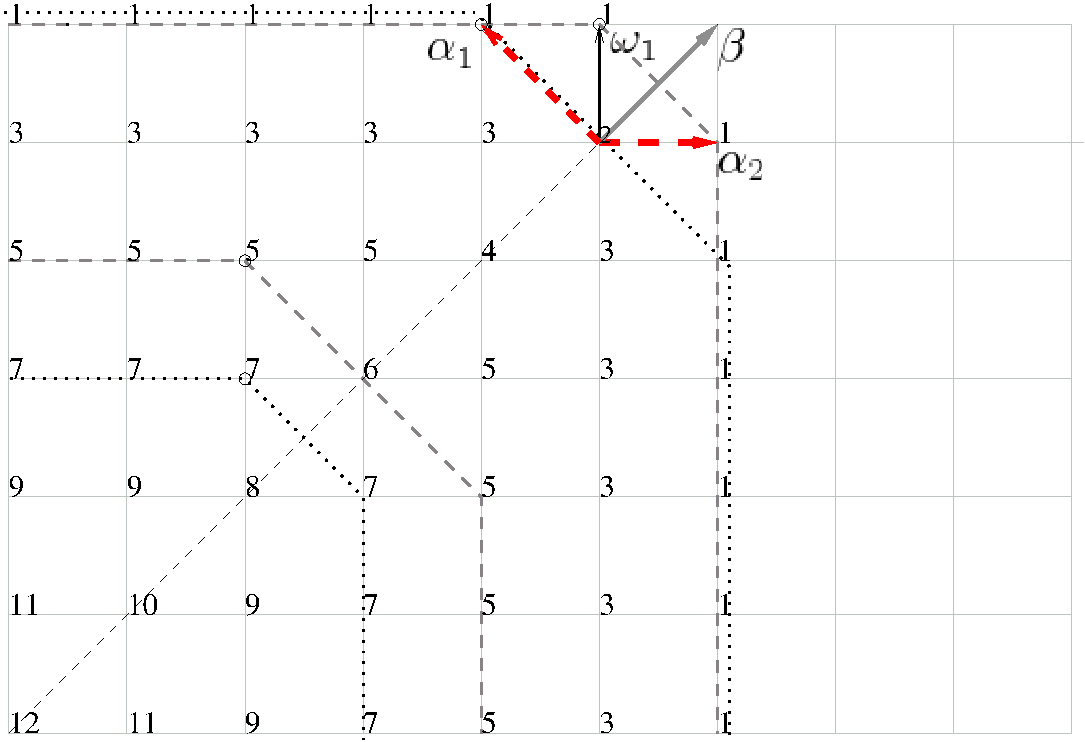
\includegraphics[width=120mm]{B2_Gen_Verma_Decomp}
  }
  \caption{Обобщенные модули Верма для регулярного вложения  $A_1$ в $B_2$. 
    Простые корни $\alpha_1, \alpha_2$ алгебры $B_2$ показаны пунктирными стрелками. Простой корень  $\beta = \alpha_1+2\alpha_2$ алгебры $A_1$ изображен серым вектором. Разложение $L^{\omega_{1}}$ представлено набором контуров входящих в него обобщенных модулей Верма. Пунктирные контуры соответствуют положительным значениям  $\epsilon(u)$, а точечные -- отрицательным. }

 \label{fig:B2_Verma_Decomp}
\end{figure}

\end{example}

\begin{remark}
Как доказано, например, в книге  \cite{humphreys2008representations} (см. утверждение 9.6), характеры обобщенных модулей Верма $M_{I}^{\mu _{\frak{a}_{\perp }}\left( u\right) }$ могут также описываться как линейные комбинации обычных модулей Верма алгебры $\frak{g}$:
\begin{equation*}
\mathrm{ch}M_{I}^{\mu _{\frak{a}_{\perp }}\left( u\right) }=\sum_{w\in W_{%
\frak{a}_{\perp }}}\epsilon \left( w\right) \mathrm{ch}M^{w\left( \mu _{%
\frak{a}_{\perp }}\left( u\right) +\rho _{\frak{a}_{\perp }}\right) -\rho _{%
\frak{a}_{\perp }}}
\end{equation*}
Подставляя это выражение в формулу (\ref{char in gen verma mod}) и используя определения  (\ref{eq:136}) и (\ref{defect-perp}), мы восстанавливаем стандартное разложение Вейля-Верма для характера:
\begin{equation*}
\mathrm{ch}\left( L^{\mu }\right) =\sum_{w\in W}\;\epsilon (u)\mathrm{ch}%
M^{w\left( \mu +\rho \right) -\rho }.
\end{equation*}
\end{remark}

\section{БГГ резольвента и ветвление}
В работе \cite{lepowsky1977generalization} показано, что для модуля старшего веса $L^{\mu }$, где $\mu \in P^{+}$, последовательность (обобщенная БГГ резольвента)
\begin{equation}
0\rightarrow M_{r}^{I}\overset{\delta _{r}}{\rightarrow }M_{r-1}^{I}\overset{%
\delta _{r-1}}{\rightarrow }\ldots \overset{\delta _{1}}{\rightarrow }%
M_{0}^{I}\overset{\varepsilon }{\rightarrow }L^{\mu }\rightarrow 0,
\label{resolution sequence}
\end{equation}
где
\begin{equation}
M_{k}^{I}=\bigoplus_{u\in U,\;\mathrm{length}\left( u\right)
=k}M_{I}^{u\left( \mu +\rho \right) -\rho },\quad M_{0}^{I}=M_{I}^{\mu }
\label{Verma elements sequence}
\end{equation}
является точной и формула (\ref{gen Weyl-Verma}%
) следует из этого разложения.

\begin{figure}[h!bt]
 \noindent\centering{
   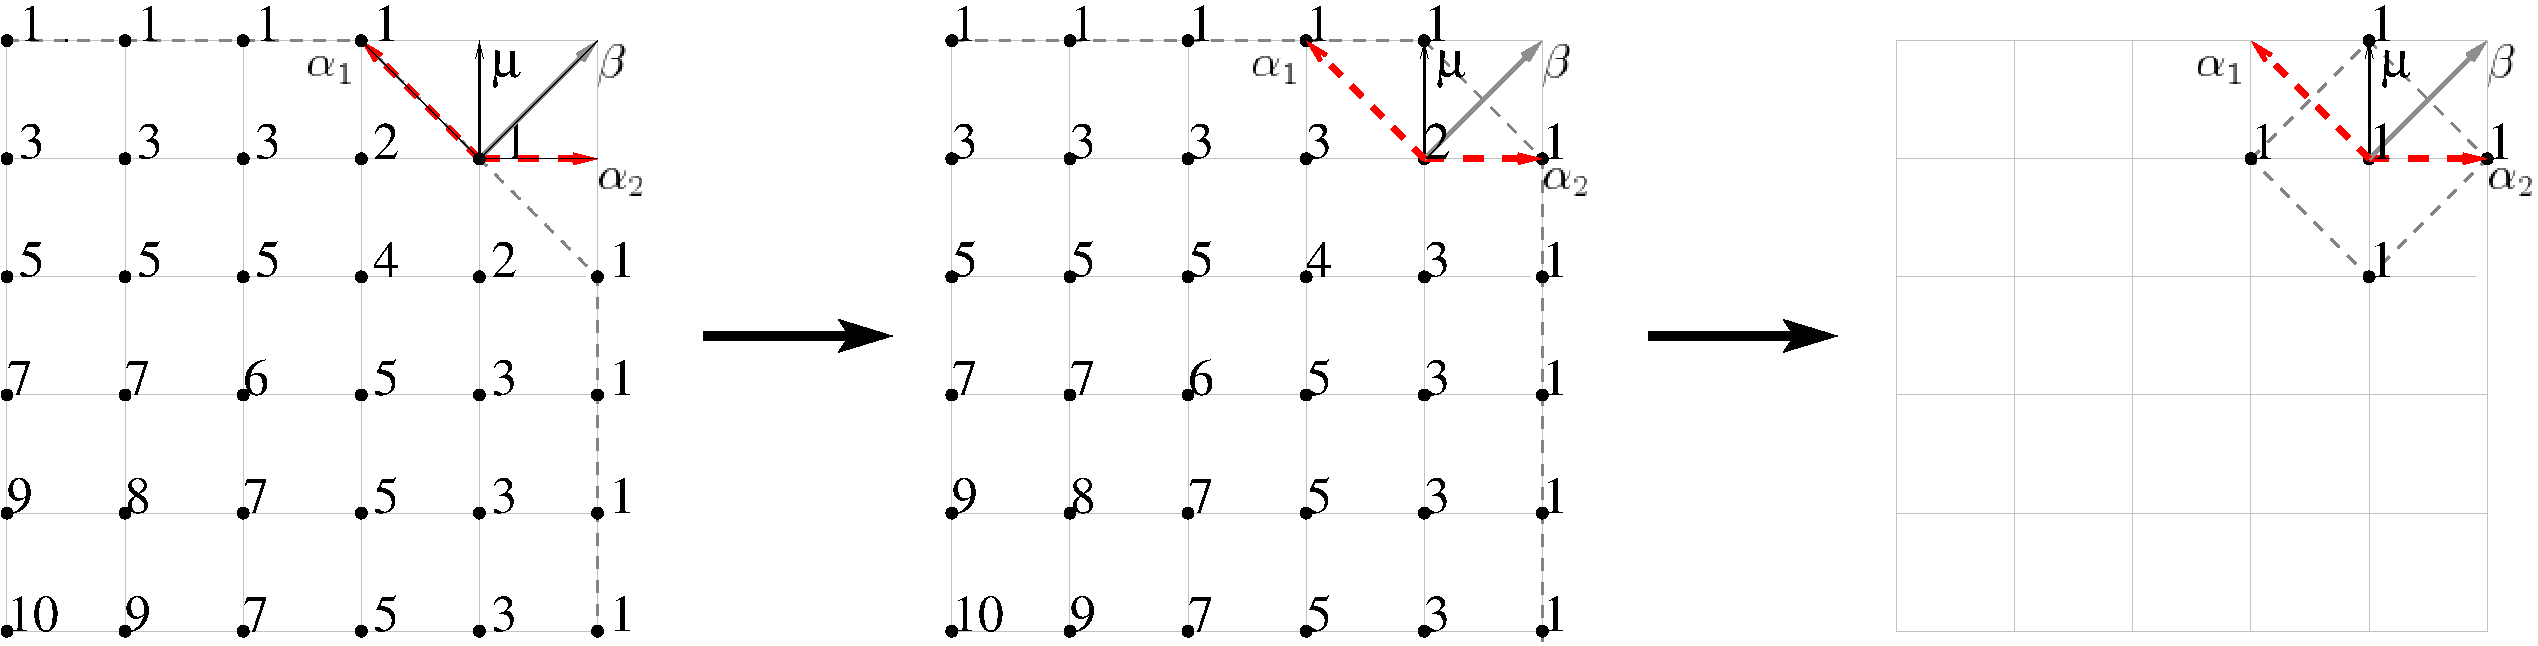
\includegraphics[width=140mm]{B2_Exact}}
 \caption{Вложение $A_1\hookrightarrow B_2$ (см. Рисунок \ref{fig:B2_Verma_Decomp}). Ортогональный партнер, подалгебра $A_1$, соответствует корню $\alpha_1$.
   Резольвента простого модуля $L^{\omega_1}$. Показана центральная часть точной последовательности
   $0 \to Im(\delta_2) \to \left( e^{\mu _{\widetilde{%
\frak{a}}}\left( e\right) }\mathrm{ch}M_{I}^{\pi _{\afb}\left[ \omega_1 \right] -%
\mathcal{D}_{\afb} }=M^{\omega_1}_{I}\right) \to
   L^{\omega_1}\to 0 $.  Здесь $\mu _{\widetilde{\frak{a}}}\left( e\right) =\pi _{\aft}\left[ \mu \right] + \mathcal{D}_{\afb}$.
   }
\end{figure}


\begin{statement}
Пусть $L^{\mu }$ --  $\frak{g}$-модуль со старшим весом $\mu \in P^{+}$, и пусть регулярная подалгебра  $\afb\hookrightarrow \frak{g}$ является ортогональным партнером редуктивной подалгебры $\frak{a}\hookrightarrow \frak{g}$. Тогда разложение (\ref{sing decomp main}) определяет как обобщенную резольвенту $L^{\mu }$ по отношению к $\afb$, так и правила ветвления $L^{\mu }$ по отношению к $\afb$, так и правила ветвления $L^{\mu }$ по отношению к $\af$ .
\end{statement}

\begin{proof}
Положим
\begin{equation*}
\mathrm{ch}M_{I}^{u\left( \mu +\rho \right) -\rho }=e^{\mu _{\widetilde{%
\frak{a}}}\left( u\right) }\mathrm{ch}M_{I}^{\mu _{\frak{a}_{\perp }}\left(
u\right) },\mathrm{ch}M_{I}^{\mu }=e^{\mu _{\widetilde{\frak{a}}}\left(
e\right) }\mathrm{ch}M_{I}^{\pi _{\frak{a}_{\perp }}\left[ \mu \right] -%
\mathcal{D}_{\frak{a}_{\perp }}},
\end{equation*}
где \ $\mu _{\widetilde{\frak{a}}}\left( u\right) ,\mu _{\frak{a}_{\perp
}}\left( u\right) $ и $\mathcal{D}_{\frak{a}_{\perp }}$ заданы как в Лемме \ref{Psi-decomp-lemma}, $%
u\in U$ определено формулой (\ref{U-def}). В результате получим элементы фильтрующей последовательности (\ref{resolution sequence}).

Рассмотрим множество $\left\{ \mu _{\frak{a}_{\perp }}\left( u\right) |u\in U\right\} $ как множество старших весов простых модулей $L_{\frak{a}%
_{\perp }}^{\mu _{\frak{a}_{\perp }}\left( u\right) }$ и вычислим размерности этих модулей. Вместе с 
$\left\{ \mu _{\widetilde{\mathfrak{a}}}\left( u\right) |u\in
U\right\} $ мы получим набор сингулярных весов
\begin{equation*}
\left\{ \epsilon (u)\;
e^{\mu _{\widetilde{\mathfrak{a}}}\left( u\right) }
\dim \left( L_{\frak{a}_{\perp }}^{\mu _{\frak{a}_{\perp
}}\left( u\right) }\right) \right\} .
\end{equation*}
Ветвление  $L_{\frak{g}\downarrow \frak{a}}^{\mu }=\bigoplus\limits_{\nu
\in P_{\frak{a}}^{+}}b_{\nu }^{\left( \mu \right) }L_{\frak{a}}^{\nu }$  определяется веером вложения  $\Gamma _{\frak{a}\rightarrow \frak{g}}$ и соотношением (\ref{recurrent-relation}), которое дает нам коэффициенты  $k_{\xi
}^{\left( \mu \right) }$, а значит определяет и  $b_{\nu }^{\left( \mu \right) }$, так как  $b_{\nu }^{\left( \mu \right) }=k_{\nu }^{\left( \mu
\right) }$ при $\nu \in \overline{C_{\frak{a}}}$ .
\end{proof}

\begin{corollary}
Пусть  $L^{\mu }$ --  $\frak{g}$-модуль со старшим весом $\mu \in P^{+}$ и  $\frak{a}\hookrightarrow \frak{g}$ -- редуктивная подалгебра $\frak{g}$. Пусть $\frak{a}_{\perp }$ -- ортогональный партнер для $\frak{a}$, -- эквивалентен  $A_{1}$, $\frak{a}_{\perp }\approx $ $A_{1}$, и $\widetilde{\frak{a}}=\frak{a}\oplus \frak{h}_{\perp }$ с $\frak{h=\frak{h}_{\frak{a}}}\oplus \frak{h}_{\frak{a}_{\perp }}\oplus \frak{h}_{\perp }$. Пусть $L_{\frak{g}\downarrow \widetilde{\frak{a}}}^{\mu }=\bigoplus\limits_{\nu \in P_{\widetilde{\frak{a}}}^{+}}b_{\nu }^{\left( \mu \right) }L_{\widetilde{\frak{a}}}^{\nu }$ -- ветвление модуля $L^{\mu }$ относительно подалгебры $\widetilde{\frak{%
a}}$. Тогда коэффициенты $b_{\nu }^{\left( \mu \right) }$ определяют обобщенную резольвенту (\ref{resolution sequence}) модуля $L^{\mu }$
по отношению к  $\frak{a}_{\perp }$.
\end{corollary}

\begin{proof}
Пусть $\alpha $ -- простой корень  $A_{1}$. Используем преобразования из группы Вейля чтобы перевести его в некоторый простой корень алгебры $\frak{g}$, например $\alpha _{1}$. Построим сингулярный элемент для модуля  $L_{\frak{g}\downarrow
\widetilde{\frak{a}}}^{\mu }$, то есть  $\Psi _{\widetilde{\frak{a}}%
}^{\left( L_{\frak{g}\downarrow \widetilde{\frak{a}}}^{\mu }\right)
}=\sum_{\nu \in P_{\widetilde{\frak{a}}}^{+},b_{\nu }^{\left( \mu \right)
}>0}b_{\nu }^{\left( \mu \right) }\Psi _{\widetilde{\frak{a}}}^{\left( \nu
\right) }$, и разложим его $\Psi _{\widetilde{\frak{a}}}^{\left( L_{\frak{%
g}\downarrow \widetilde{\frak{a}}}^{\mu }\right) }=k_{\xi }^{\left( \mu
\right) }e^{\xi }$. В нашем случае представители $u$ в рекуррентном соотношении (\ref{recurrent-relation}) определяются весом $\xi $ однозначно:
\begin{equation*}
\epsilon (u\left( \xi \right) )\;\dim \left( L_{\frak{a}_{\perp }}^{\mu _{%
\frak{a}_{\perp }}\left( u\left( \xi \right) \right) }\right) =-s\left(
\gamma _{0}\right) k_{\xi }^{\left( \mu \right) }-\sum_{\gamma \in \Gamma _{%
\widetilde{\frak{a}}\rightarrow \frak{g}}}s\left( \gamma +\gamma _{0}\right)
k_{\xi +\gamma }^{\left( \mu \right) }.
\end{equation*}
Тогда
\begin{equation*}
\dim \left( L_{\frak{a}_{\perp }}^{\mu _{\frak{a}_{\perp }}\left( u\left(
\xi \right) \right) }\right) =\left| s\left( \gamma _{0}\right) k_{\xi
}^{\left( \mu \right) }+\sum_{\gamma \in \Gamma _{\widetilde{\frak{a}}%
\rightarrow \frak{g}}}s\left( \gamma +\gamma _{0}\right) k_{\xi +\gamma
}^{\left( \mu \right) }\right|
\end{equation*}
и
\begin{equation*}
\mu _{\frak{a}_{\perp }}\left( u\left( \xi \right) \right) =\frac{1}{2}%
\left( \dim \left( L_{A_{1}}^{\mu \left( \xi \right) }\right) -1\right)
\alpha _{1}
\end{equation*}
Таким образом, множество обобщенных модулей Верма  $e^{\xi +\mathcal{D}%
_{\frak{a}_{\perp }}}\mathrm{ch}M_{I}^{\mu _{\frak{a}_{\perp }}\left(
u\left( \xi \right) \right) }$ полностью фиксировано:
\begin{equation*}
\left\{ e^{\mu _{\widetilde{\mathfrak{a}}}\left( u\right) }\mathrm{ch}%
M_{I}^{\mu _{\frak{a}_{\perp }}\left( u\right) }|u\in U\right\} .
\end{equation*}
Упорядочивая эти модули по длине $u$, мы получаем компоненты (\ref{Verma elements sequence}) резольвенты (\ref{resolution sequence}).
\end{proof}



\section{Заключение}

\label{sec:conclusions}
В главе \ref{cha:affine-lie-algebras}  было показано, что метод веера вложения работает также и для специальных вложений. Надо заметить, что  разложения Вейля-Верма также могут быть получены в этом случае. Резольвенты, соответствующие специальным подалгебрам, описывают соотношения между проекциями характера начального модуля и обобщенными модулями Верма со старшими весами в подпространстве $h^*$.

Рассмотрим ситуацию, когда выбор простых корней зафиксирован какими-то внешними факторами (возникающими, например, из требований физических приложений). В этом случае ортогональный партнер не может порождаться только простыми корнями. Элементы   $\frak{u}_{I}^{+}:=\sum_{\eta \in \Delta
^{+}\setminus \Delta _{I}^{+}}\frak{g}_{\eta }$ не образуют подалгебру в  $%
\mathfrak{g}$, так как некоторые не простые корни отсутствуют в  $\Delta ^{+}\setminus
\Delta _{I}^{+}$. Важно отметить, что в этом случае формула Вейля-Верма по-прежнему существует. В ней обобщенные модули Верма соответствуют сжатиями \cite{Doebner1967Melsheimer} алгебры $%
\frak{n}^{+}$ и соотношения Вейля-Верма описывают разложение пространства представления $L^{\mu}$ в набор обобщенных модулей Верма сжатой алгебры  $U\left(\frak{n}_c^{+}\right)$. Весовые векторы образованы базисом Пуанкаре-Биркгофа-Витта алгебр $U\left(\frak{n}_c^{+}\right)$ и
$U\left( \mathfrak{a}_{\bot} \right)$. Чтобы рассмотреть такое пространство как  $%
\mathfrak{g}$-модуль мы должны выполнить деформацию \cite
{Nijenhuis1966Richardson} алгебры $\frak{n}_c^{+}$ (то есть восстановить первоначальный закон композиции). Пространство сохраняется, и после такой деформации генераторы начальной алгебры будут действовать на нем правильным образом.



%%
%% End of file
%%% Local Variables: 
%%% mode: latex
%%% TeX-master: "thesis"
%%% End: 

\chapter{Конформная теория поля}
\label{cha:cft}

Подробное изложение \cite{difrancesco1997cft}. 

\section{Общие свойства}
\label{sec:cft-general}
Алгебра Вирасоро. Представления алгебры Вирасоро. Модулярная инвариантность.

\section{Модели Весса-Зумино-Новикова-Виттена}
\label{sec:wzw}
Связь с аффинными алгебрами Ли.
Конформные вложения и недиагональные модулярные инварианты. 

\section{Coset-модели}
\label{sec:coset-models}
Ветвления. Функции ветвления и статсуммы. 
Калибровочные WZW-модели. 

\section{SLE}
\label{sec:sle}
SLE на WZW-моделях. Граничные условия. Парафермионы. SLE на coset-моделях.

%%% Local Variables: 
%%% mode: latex
%%% TeX-master: t
%%% End: 

\chapter{Практические приложения}
\label{cha:applications}

В этой главе мы рассматриваем роль сингулярных элементов модулей аффинных алгебр Ли в приложениях к задачам конформной теории поля. Мы используем установленные в главах \ref{cha:affine-lie-algebras}, \ref{cha:BGG}, \ref{cha:splints} свойства для эффективных вычислений. 

\section{Coset-модели и критическое поведение}

% и  Эволюция Шрамма-Левнера и алгебраические свойства предельного перехода от решеточных моделей к конформной теории поля}
\label{sec:SLE}

Алгебраические методы в конформной теории поля позволяют получать явные уравнения на корреляционные функции (например, уравнения Книжника-Замолодчикова \eqref{eq:66} в ВЗНВ-моделях и их аналоги в coset-моделях \eqref{eq:101}). Во многих случаях эти уравнения можно решить аналитически либо численно и получить конкретные значения для физических величин, например, для критических индексов. Таким образом конформная теория поля является мощным инструментом для описания критического поведения в решеточных моделях. 

Однако соответствие между решеточными моделями и конформной теорией поля, описывающей их критическое поведение, не так легко установить. В случае простых моделей (Изинга, Поттса, Ашкина-Теллера и т.д.) и минимальных моделей конформной теории поля такое соответствие первоначально устанавливалось путем сравнения центральных зарядов и конформных размерностей. Но соответствие корреляторов нуждается в строгом доказательстве. Один из инструментов изучения решеточных моделей -- эволюция Шрамма-Левнера -- позволяет в некоторых случаях доказать такое соответствие (см. \cite{duminil2011conformal,chelkak2009universality,smirnov2007towards,smirnov2001critical,Cardy:2005kh,bauer2004conformal,bauer2004sle,bauer2004cfts,bauer2003sle,friedrich2003conformal,bauer2002sle}). Класс моделей конформной теории поля, для которых получены такие результаты, в основном ограничивается минимальными унитарными моделями. 

Эволюция Шрамма-Левнера -- это стохастический процесс, который предложил Oded Schramm  \cite{schramm2000scaling} для описания скейлингового предела критических интерфейсов в двумерных статистических решеточных моделях. Этот подход к критическим системам дал много строгих результатов в теории критического поведения (см. обзоры  \cite{rohde2005basic}, \cite{bauer20062d}, \cite{Cardy:2005kh}). В разделе \ref{sec:schr-loewn-evol} мы приводим необходимые определения.  

Вероятностная мера, порожденная эволюцией Шрамма-Левнера на случайных кривых, конформно-инвариантна. Так как конформная теория поля представляет собой другой метод для изучения двумерных критических систем, естественно изучать ее связь с эволюцией Шрамма-Левнера. Такая связь изучалась, например, в работах \cite{bauer2004conformal,bauer2004cfts,bauer2003sle,bauer2002sle} (и многих других), но в основном для минимальных унитарных моделей. 
Идея состоит в рассмотрении определенных наблюдаемых в области с разрезом. Эта конструкция обсуждается в разделе \ref{sec:corr-betw-sle}. 

Как мы показали в главе \ref{cha:CFT}, более общие модели конформной теории поля обладают дополнительными симметриями. Так в моделях Весса-Зумино-Новикова-Виттена и в coset-моделях возникают аффинные алгебры Ли.  Чтобы реализовать эти симметрии при изучении эволюции Шрамма-Левнера, нужно ввести дополнительное случайное блуждание на группе Ли \cite{bettelheim2005stochastic}, \cite{Rasmussen:2004xr}. Такое случайное блуждание определяется в разделе \ref{sec:sle-wzw-models}. Соответствие между мартингалами эволюции Шрамма-Левнера и корреляционными функциями в моделях Весса-Зумино-Новикова-Виттена изучалось в работе \cite{alekseev2010sle}. Аналогичное обобщение на $\mathbb{Z}(N)$-парафермионную модель было предложено в статьях \cite{santachiara2008sle,picco2008numerical}. 

Мы обобщаем эволюцию Шрамма-Левнера с дополнительным случайным блужданием на группе Ли на случай фактор-пространства  $G/A$ и в изучении связи с coset-конструкцией конформной теории поля. По аналогии со случаем моделей Весса-Зумино-Новикова-Виттена мы получаем систему алгебраических уравнений на оператор смены граничного условия из условия на мартингал. 
При помощи coset-конструкции можно реализовать минимальные и парафермионные модели конформной теории поля (см. \cite{difrancesco1997cft}).  Мы сравниваем наши уравнения на оператор смены граничных условий с результатами работы \cite{santachiara2008sle} и видим, что они совпадают. Кроме того, полученные нами значения параметров эволюции Шрамма-Лёвнера согласуются с результатами для минимальных моделей.

%%  В разделе  \ref{sec:5-conclusion} мы обсуждаем возможность сравнения классификации операторов смены граничных условий, следующей из свойства мартингалов с общей классификацией операторов смены граничных условий в граничной конформной теории поля, связанной с D-бранными решениями \cite{fuchs2005geometry,fredenhagen2002d,elitzur2002d,Maldacena:2001ky,felder1999geometry,alekseev1999d}. 
%%  

\subsection{Эволюция Шрамма-Левнера}
\label{sec:schr-loewn-evol}
Рассмотрим модель Изинга на треугольной решетке в верхней полуплоскости (см. Рисунок \ref{fig:sle}). Наложим следующее граничное условие: потребуем, чтобы на одной половине границы все спины были направлены вверх, а на другой половине -- вниз. Тогда при любой конфигурации спинов на полуплоскости будет интерфейс, разделяющий два кластера и соединяющий точку ноль с бесконечностью (см. Рисунок \ref{fig:sle}).

\begin{figure}[h]
  \centering{
    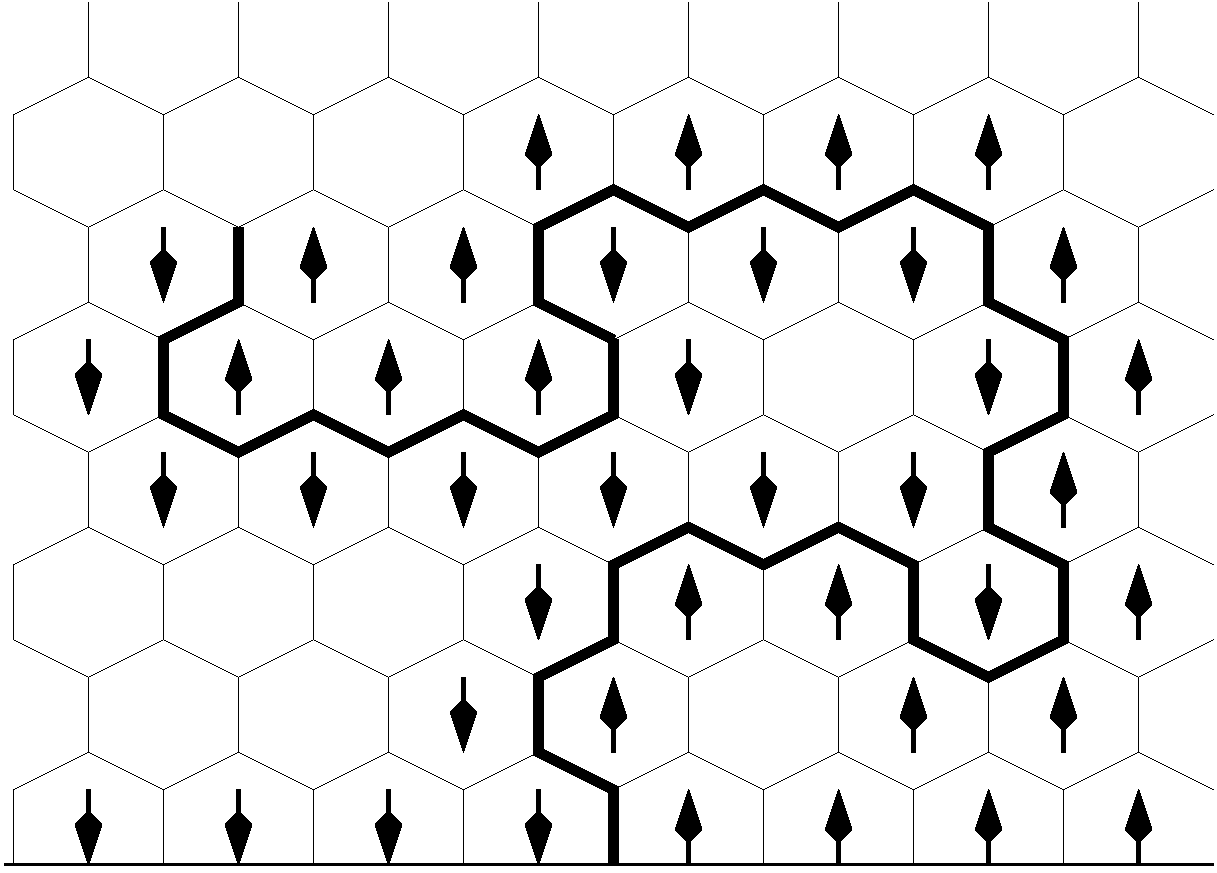
\includegraphics[height=50mm]{explore}
    \caption{Интерфейс в модели Изинга на треугольной решетке}}
  \label{fig:sle}
\end{figure}
Мы можем наложить условие существования части интерфейса конечной длины и рассмотреть конфигурации статистической модели, удовлетворяющие этому условию. Очевидно, такие конфигурации эквивалентны конфигурациям модели на области с разрезом вдоль интерфейса. 

Теперь рассмотрим непрерывный предел решеточной модели с (частью) интерфейса конечной длины. Интерфейсы в случайных конфигурациях модели сходятся к случайной кривой. Старая гипотеза \cite{Polyakov:1970xd} о конформной инвариантности в критической точке была недавно строго доказана для некоторых решеточных моделей (см. \cite{smirnov2007towards}, \cite{duminil2011conformal}). Мы предполагаем наличие конформной инвариантности в критической точке и рассматриваем верхнюю полуплоскость  $\mathbb{H}$ с разрезом вдоль критического интерфейса  $\gamma_{t}$. Такую область с разрезом мы обозначим через  $\mathbb{H}_{t}=\mathbb{H}\setminus \gamma_{t}$. Конформное отображение из $\mathbb{H}_{t}$ в $\mathbb{H}$ обозначим через $g_{t}:\mathbb{H}_{t}\to \mathbb{H}$ (см. Рисунок \ref{fig:sle2}).

\begin{figure}[h]
  \centering{
    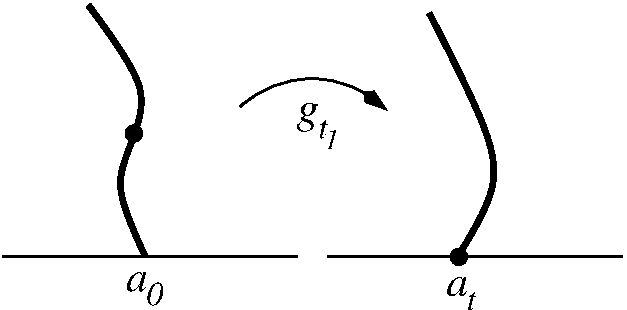
\includegraphics[width=60mm]{loewner}
    \caption{Конформное отображение $g_{t}(z):\mathbb{H}_{t}\to \mathbb{H}$.}}
  \label{fig:sle2}
\end{figure}

В статье \cite{schramm2000scaling} было показано, что  $g_{t}(z)$ удовлетворяет стохастическому дифференциальному уравнению
\begin{equation}
\label{eq:166}
  \frac{\partial g_t(z)}{\partial t} = \frac{ 2}{g_t(z)-\sqrt{\kappa}\xi_{t}} ,
\end{equation}
здесь $\xi_{t}$ -- Броуновское движение. Динамика конца  $z_{t}$ критической кривой $\gamma_{t}$ (конец следа эволюции Шрамма-Левнера) описывается уравнением $z_{t}=g_{t}^{-1}(\sqrt{\kappa}\xi_{t})$. 

Стохастический процесс, который удовлетворяет уравнению \eqref{eq:166} называется {\it эволюцией Шрамма-Левнера} на верхней полуплоскости $\mathbb{H}$. Для нас будет удобнее использовать отображение $w_{t} (z)=g_{t}(z)-\sqrt{\kappa}\xi_{t}$, так что уравнение \eqref{eq:166} переписывается в виде
\begin{equation}
  \label{eq:120}
       d w _{t}= \frac{2dt}{w_{t} }-\sqrt{\kappa}\xi_{t}  
\end{equation}
Эволюция Шрамма-Левнера порождает конформно-инвариантную вероятностную меру на кривых $\gamma_{t}$ в $\mathbb{H}$.

\subsection{Мартингалы эволюции Шрамма-Левнера и корреляционные функции в конформной теории поля}
\label{sec:corr-betw-sle}

Теперь рассмотрим наблюдаемые в присутствии следа эволюции Шрамма-Левнера. Математическое ожидание решеточной наблюдаемой $\mathcal{O}$ на верхней полуплоскости можно вычислить как сумму ожиданий этой наблюдаемой в присутствии (конечной части) траектории эволюции Шрамма-Левнера  $\gamma_{t}$ вплоть до некоторого времени $t$, умноженных на вероятность этой траектории:
\begin{equation*}
  \prec \mathcal{O} \succ_{\mathbb{H}}=\mathbb{E}\left[\prec\mathcal{O}\succ_{\gamma_{t}}\right]=\sum_{\gamma_{t}} P\left[C_{\gamma_{t}}\right] \prec \mathcal{O} \succ_{\gamma_{t}}
\end{equation*}
Решеточная наблюдаемая  $\prec \mathcal{O} \succ_{\mathbb{H}}$ не зависит от  $t$, следовательно $\prec\mathcal{O}\succ_{\gamma_{t}}$ -- мартингал.

В непрерывном пределе решеточные наблюдаемые сходятся к корреляционным функциям в конформной теории поля \cite{bauer2003sle,bauer2003conformal,bauer2002sle}. Мы должны учесть изменение граничных условий на конце следа эволюции Шрамма-Левнера и на бесконечности, так что соотношение имеет вид:
\begin{equation}
  \prec \mathcal{O} \succ_{\mathbb{H}_{t}}\to \mathcal{F}(\left\{z_{i}\right\})_{\mathbb{H}_{t}}=
  \frac{\left< \mathcal{O}(\{z_{i}\})\phi(z_{t})\phi^{\dagger}(\infty)\right>_{\mathbb{H}_{t}}}{\left<\phi(z_{t})\phi^{\dagger}(\infty)\right>_{\mathbb{H}_{t}}}
%% =
%%   \frac{\left<^{g_{t}}
%% \mathcal{O}\phi(\xi_{t})\phi^{\dagger}(\infty)\right>_{\mathbb{H}}}{\left<\phi(\xi_{t})\phi^{\dagger}(\infty)\right>_{\mathbb{H}}}
\label{eq:162}
\end{equation}

%% Here $\phi(z_{t})$ is a primary field corresponding to boundary condition changing operator.
%% We've used the conformal map $g_{t}$ to get the expression on the whole plane in equation \eqref{eq:162}.
Мы рассматриваем теорию с границей, так что мы должны использовать модели граничной конформной теории поля и накладывать соответствующие граничные условия \cite{cardy1984conformal,cardy1989boundary,cardy1991bulk}. В случае верхней полуплоскости корреляционные функции в граничной конформной теории поля могут быть переписаны как корреляционные функции для теории на всей плоскости, но с удвоенным числом полей (см. раздел \ref{sec:boundary-cft}).

% Here we are interested mainly in properties of boundary condition changing operator $\phi$. 

Мы предполагаем, что $\mathcal{F}$ содержит некоторый набор примарных полей  $\varphi_{i}$ с конформными весами $h_{i}$. Так как мы рассматриваем граничную конформную теорию поля, мы должны добавить объемные поля в сопряженных точках  $\bar z_{i}$.  Кроме того, у нас есть операторы смены граничного условия   $\phi$ на конце следа эволюции Шрамма-Левнера и на бесконечности. Воспользуемся конформным отображением   $w(z):\mathbb{H}\setminus\gamma_{t}\to \mathbb{H}$, чтобы переписать выражение \eqref{eq:162} на верхней полуплоскости без разреза:
\begin{equation}
  \mathcal{F}(\left\{z_{i}\right\})_{\mathbb{H}_{t}}=\prod \left(\frac{\partial w(z_{i})}{\partial z_{i}}\right)^{h_{\lambda_i}} 
  \prod \left(\frac{\partial \bar w(\bar z_{i})}{\partial \bar z_{i}}\right)^{h_{\lambda^{*}_i}}
  \mathcal{F}(\left\{w_{i}, \bar w_{i}\right\})_{\mathbb{H}}
  \label{eq:69}
\end{equation}

Теперь нам нужно рассмотреть, как преобразуется конец следа эволюции Шрамма-Левнера  $\gamma_{t}$ при переходе от времени $t$ к $t+ dt$. Первый множитель в правой части уравнения  (\ref{eq:69}) дает нам
\begin{equation*}
  -\frac{2h_{\lambda_{i}}}{w_{i}^{2}}\left(\frac{\partial w_{i}}{\partial z_{i}}\right)^{h_{i}}.
\end{equation*}
Для преобразования примарных полей  $\varphi_{\lambda_{i}}$ имеет место равенство
\begin{equation}
\label{eq:70}
  d\varphi_{i}(w_{i}) = \mathcal{G}_{i}\varphi_{i}(w_{i})=\left(\frac{2dt}{w_{i}}-\sqrt{\kappa} d\xi_{t}\right) \partial_{w_{i}}\varphi_{i}(w_{i}) 
\end{equation}
Мы обозначим генератор этого преобразования через  $\mathcal{G}_{i}$.

Так как $ \prec\mathcal{O}\succ_{\gamma_{t}}$ --  мартингал, математическое ожидание его приращения при эволюции от  $t$ к $t+dt$ равняется нулю
\begin{equation}
  \mathbb{E}\left[\prec\mathcal{O}\succ_{\gamma_{t}}\right]=    \mathbb{E}\left[\prec\mathcal{O}\succ_{\gamma_{t+dt}}\right], \quad d\mathbb{E}\left[ \prec\mathcal{O}\succ_{\gamma_{t}}\right]=0
\label{eq:163}
\end{equation}
Используем исчисление Ито и получим выражение для дифференциала $\mathcal{F}$:
\begin{equation}
d \mathcal{F}_{\mathbb{H}_{t}}= \left(\prod_{i=1}^{2N}\left(\frac{\partial w_{i}}{\partial z_{i}}\right)^{h_{i}}\right)\left(-\sum_{i=1}^{2N}\frac{2h_{i}dt}{w_{i}^{2}}+\left[\sum_{i=1}^{2N}\mathcal{G}_{i}+\frac{1}{2}
      \sum_{i,j}\mathcal{G}_{i}\mathcal{G}_{j}\right]\right)\mathcal{F}_{\mathbb{H}}=0
\label{eq:150}
\end{equation}
Подставим формулу \eqref{eq:70} и получим уравнение
\begin{equation}
  \left( \sum_{i}\left[-\frac{2h_{i}}{w_{i}^{2}} +\frac{2}{w_{i}}\partial_{w_{i}}\right]+\frac{\kappa}{2}\sum_{i,j}\partial_{w_{i}} \partial_{w_{j}}\right)\mathcal{F}(\left\{z_{i}\right\})=0
\label{eq:165}
\end{equation}

Для корреляционных функций вторичных полей  $L_{-n}\phi$ имеет место уравнение
\begin{equation}
\left< (L_{-n}\phi)(z) \varphi_{1}\dots \varphi_{N}\right>=\mathcal{L}_{-n}\left<\phi\varphi_{1}\dots\varphi_{N}\right>,
\end{equation}
где $n\geq 1$ и
\begin{equation*}
  \mathcal{L}_{-n}=\sum_{i=1}^{N} \left(\frac{(n-1)h_{i}}{(w_{i}-z)^{n}} -\frac{1}{(w_{i}-z)^{n-1}}\partial_{w_{i}}\right)
\end{equation*}
(См. \cite{difrancesco1997cft}). То есть мы можем переписать дифференциальное уравнение \eqref{eq:165} как алгебраическое уравнение на поле $\phi$, соответствующее оператору смены граничных условий:
\begin{equation}
  \label{eq:168}
   \left<\left([L_{-2}-\frac{\kappa}{2}L_{-1}^{2}]\phi\right)(0)\; \varphi_{1}\dots \varphi_{2N}\right>=0.
\end{equation}
В случае минимальных моделей набор примарных полей конечен и все состояния можно получить через соответствие между полями и состояниями
\cite{belavin1984ics}, \cite{difrancesco1997cft}. 
Равенство \eqref{eq:168} верно для произвольной наблюдаемой $\mathcal{O}$ и для произвольных примарных поле $\varphi_{i}$, так что $\psi=[L_{-2}-\frac{\kappa}{2}L_{-1}^{2}]\phi$ -- нулевое поле уровня два и $\psi(0)\left|0\right>$ -- нулевое состояние уровня два. В минимальных унитарных моделях существует только два примарных поля, порождающих модули Верма алгебры Вирасоро с нулевыми состояниями на уровне два. Это поля $\phi_{1,2}$ и $\phi_{2,1}$, так что $\phi\sim \phi_{1,2} \;\text{или}\; \phi_{2,1}$. 

\subsection{Модели Весса-Зумино-Новикова-Виттена и эволюция Шрамма-Левнера}
\label{sec:sle-wzw-models}
Чтобы обобщить анализ предыдущего раздела  \ref{sec:corr-betw-sle} на не-минимальные модели мы должны принять во внимание дополнительные симметрии. Модели Весса-Зумино-Новикова-Виттена обладают симметрией Каца-Муди в дополнение к конформной инвариантности, приводящей к появлению алгебры Вирасоро. Мы описали ВЗНВ-модели в разделе \ref{sec:WZNW-models}. 

Рассмотрим эволюцию Шрамма-Левнера в ВЗНВ-моделях. 
Подобно минимальным моделям мы рассматриваем наблюдаемые
\begin{equation*}
  \mathcal{F}(\left\{z_{i}\right\})_{\mathbb{H}_{t}}=
  \frac{\left<\phi_{\Lambda}(z_{t}) \varphi_{\lambda_1}(z_{1}) \dots \varphi_{\lambda_n}(z_{n}) \varphi_{\lambda^{*}_1}(\bar z_{1}) \dots \varphi_{\lambda^{*}_n}(\bar z_{n})
      \phi_{\Lambda^{*}}(\infty)\right>}{\left<\phi_{\Lambda}(z_{t})\phi_{\Lambda^{*}}(\infty)\right>},
\end{equation*}
где примарные объемные поля нумеруются весами $\lambda_i$.

Мы опять используем конформное отображение  $w(z):\mathbb{H}\setminus\gamma_{t}\to \mathbb{H}$ чтобы переписать формулу для наблюдаемых на всей верхней полуплоскости.
\begin{equation}
  \mathcal{F}(\left\{z_{i}\right\})_{\mathbb{H}_{t}}=\prod \left(\frac{\partial w(z_{i})}{\partial z_{i}}\right)^{h_{\lambda_i}} 
  \prod \left(\frac{\partial \bar w(\bar z_{i})}{\partial \bar z_{i}}\right)^{h_{\lambda^{*}_i}}
  \mathcal{F}(\left\{w_{i}, \bar w_{i}\right\})_{\mathbb{H}}
  \label{eq:177}
\end{equation}

В результате эволюции от $t$ к $t+dt$ первый множитель дает нам $-\frac{2h_{\lambda_{i}}}{w_{i}^{2}}\left(\frac{\partial w_{i}}{\partial z_{i}}\right)^{h_{\lambda_{i}}}$.

При рассмотрении полей нам нужно добавить случайное калибровочное преобразование  (случайное блуждание в $G$) к стохастическому процессу \cite{bettelheim2005stochastic}, \cite{alekseev2010sle}. 
Для полей мы имеем
\begin{equation*}
  d\varphi_{\lambda_{i}}(w_{i}) = \mathcal{G}_{i}\varphi_{\lambda_{i}}(w_{i}),
\end{equation*}
так что в генераторе преобразования поля появляется дополнительный член
\begin{equation}
  \mathcal{G}_{i}=\left(\frac{2dt}{w_{i}}-\sqrt{\kappa} d\xi_{t}\right) \partial_{w_{i}}+\frac{\sqrt{\tau}}{w_{i}}\sum_{a=1}^{\mathrm{dim} \gf}\left(d \theta ^{a} t^{a}_{i}\right)
\label{eq:159}
\end{equation}
Здесь  $d\theta^{a}$ -- генераторы  $\mathrm{dim}\gf$--мерного Броуновского движения, с $\mathbb{E}[d\theta^{a}d\theta^{b}]=\delta_{ab}dt$. Мы предполагаем, что $t^{a}$ -- это базис в $\gf$, ортогональный по отношению к форме Киллинга $\mathcal{K}$, $\mathcal{K}(t^{a},t^{b})=\delta_{ab}$.

Воспользуемся формулой \eqref{eq:150} и получим следующее уравнение из условий для мартингала:
\begin{equation}
  \left(-2 \mathcal{L}_{-2}+\frac{1}{2}\kappa \mathcal{L}_{-1}^{2}+\frac{1}{2}\tau\sum_{a} \mathcal{J}^{a}_{-1} \mathcal{J}^{a}_{-1}\right)        \mathcal{F}(\left\{w_{i}, \bar w_{i}\right\})_{\mathbb{H}}=0,
  \label{eq:167}
\end{equation}
где
\begin{equation*}
  \mathcal{L}_{-n}=\sum_{i}\left(\frac{(n-1)h_{\lambda_{i}}}{(w_{i}-z)^{n}}-\frac{1}{(w_{i}-z)^{n-1}}\partial_{w_{i}}\right);\quad \mathcal{J}^{a}_{{-n}}=-\sum_{i}\frac{t^{a}_{i}}{(w_{i}-z)^{n}}
\end{equation*}
Мы снова перепишем уравнение в виде алгебраического соотношения на поле, соответствующее оператору смены граничного условия. Теперь
\begin{equation}
  \left| \psi\right>=\left(-2 L_{-2}+\frac{1}{2}\kappa L_{-1}^{2}+\frac{1}{2}\tau\sum_{a} J^{a}_{-1} J^{a}_{-1}\right) \left|\phi_{\Lambda}\right>    
  \label{eq:16}
\end{equation}
является нулевым состоянием уровня два.
Из того, что корреляторы примарных полей с полем $\psi$ равны нулю следует, что состояние $\left|\psi\right>$ содержится в инвариантном подмодуле модуля Верма аффинной алгебры $\gfh$, порожденного действием операторов $J^a_n$ на состояние $\phi_{\Lambda}$, отвечающее старшему весу $\Lambda$. Таким образом, условие мартингала относительно эволюции Шрамма-Левнера эквивалентно тому, что некоторый вектор не принадлежит неприводимому модулю аффинной алгебры, а содержится в максимальном инвариантном подмодуле модуля Верма. Как видно, например, из конструкции БГГ-резольвенты (см. главу \ref{cha:BGG}), инвариантные подмодули в модуле Верма тесно связаны со структурой сингулярного элемента неприводимого модуля. 

Если на состояние $\left|\psi\right>$ подействовать повышающими операторами, мы должны получить ноль.
\begin{eqnarray}
 \label{eq:34}
 L_{1}\left|\psi\right>=0\\
  L_{2}\left|\psi\right>=0
\end{eqnarray}
В силу конструкции Сугавары (\ref{eq:91}) $  L_n=\frac{1}{2(k+h^{\vee})}\sum_a\sum_m:J^a_m J^a_{n-m}:$ это условие может быть выполнено только если $J^{a}_{n} \left|\psi\right>=0$
\begin{eqnarray}
  \label{eq:36} 
  J^{a}_{1} \left|\psi\right>=0\\
  J^{a}_{2}\left|\psi\right>=0.
\end{eqnarray}
Эти уравнения можно переписать как алгебраические соотношения, связывающие параметры случайного блуждания $\kappa, \tau$ с уровнем  $k$ представления аффинной алгебры Ли, если воспользоваться коммутационными соотношениями  (\ref{eq:102}), (\ref{eq:90}). Полный анализ таких алгебраических соотношений проведен в работе \cite{alekseev2010sle}.

Однако мы воспользуемся другим подходом. Рассмотрим состояние $\left|\psi\right>$ с точки зрения конечномерной подалгебры $\gf\subset\gfh$. Все три слагаемых, действующих на состояние $\left|\phi_{\Lambda}\right>$ в формуле (\ref{eq:16}) с точки зрения подалгебры $\gf$ являются квадратичными операторами Казимира (пропорциональны $\sum_a J^a J^a$). Поэтому состояние $\left|\psi\right>$ отвечает весу $\Lambda-2\delta$. 

Сразу можно написать необходимое условие на уровень и старший вес $\Lambda$: вектор веса  $\Lambda-2\delta$ должен содержаться в модуле Верма $V^{\mu}$, старший вес которого $\mu$ является сингулярным для неприводимого модуля $L^{\Lambda}$. То есть должны существовать неотрицательные числа $a_0,\dots,a_r\in \mathbb{Z}_+$ ($r=\mathrm{rank}(\gf)$) и отражение Вейля $w\in W_{\gfh}$ такие, что $\Lambda-2\delta = w(\Lambda+\rho)-\rho-\sum_{k=0}^r a_k \alpha_k$. 
Вспомним, что группа Вейля аффинной алгебры Ли $\gfh$  представляет собой полупрямое произведение группы Вейля конечномерной алгебры $\gf$ и группы трансляций, порожденной простыми корнями $\alpha_1,\dots,\alpha_r$. 
Так как $\alpha_0 = \delta-\theta$ получаем, что $a_0=2$

Рассмотрим некоторые примеры. 
Простейший случай, когда выполняются условия (\ref{eq:34}),(\ref{eq:36}) -- это $\gfh = \hat{\mathfrak{su}}(2),\; \Lambda=\omega_1,\; k=1,\; \forall \kappa: \tau = 2-\kappa/2$. 


\subsection{Coset-модели и эволюция Шрамма-Левнера}
\label{sec:coset-models-sle}
Теперь мы обобщим анализ соответствия между эволюцией Шрамма-Левнера и конформной теорией поля на случай coset-моделей \cite{Goddard198588}. Такие модели задаются алгеброй Ли $\gf$ и ее подалгеброй $\af$. Воспользуемся обозначениями, введенными в разделе \ref{sec:coset-models-cft}.

Как мы упоминали в главе \ref{cha:CFT}, $G/A$-coset модель конформной теории поля может быть реализована как ВЗНВ-модель (с калибровочной группой $G$), взаимодействующая с чисто калибровочными полями, с калибровочной группой $A\subset G$ \cite{gawdzki1988g,figueroa89equivalence}. Как было показано в главе \ref{cha:CFT}, действие записывается через поля  $g:\mathbb{C}\to G$ и $A,\bar A:\mathbb{C}\to \af$ (\ref{eq:38}). Здесь $\af$ -- алгебра Ли, соответствующая группе Ли $A$.

Если мы фиксируем  $A$-калибровку, у нас останется  $G/A$ калибровочная инвариантность. Значит мы должны добавить случайные калибровочные преобразования к эволюции Шрамма-Левнера, аналогично случаю ВЗНВ-моделей из предыдущего раздела (См. также \cite{bettelheim2005stochastic}).  Обозначим через $t^{a}_{i}$ ($\tilde{t}^{b}_{i}$) генераторы представления алгебры $\gf$ (соответственно, представления $\af$), соответствующего примарному полю $\varphi_{i}$.

Рассмотрим эволюцию следа SLE $\gamma_{t}$ с момента   $t$ до $t+ dt$.  Первый сомножитель в правой части уравнения (\ref{eq:177}) дает нам
\begin{equation*}
  -\frac{2h_{i}}{w_{i}^{2}}\left(\frac{\partial w_{i}}{\partial z_{i}}\right)^{h_{i}}.
\end{equation*}
Напомним, что через  $\mathcal{G}_{i}$ мы обозначили  генераторы инфинитезимальных преобразований примарных $\varphi_{i}$:$d\varphi_{i}(w_{i}) = \mathcal{G}_{i}\varphi_{i}(w_{i})$. Нормируем дополнительное $\left(\dim\gf\right)$-мерное Броуновское движение следующим образом: $\mathbb  {E}\left[d\theta^{a}\; d\theta^{b}\right]=\mathcal{K}(t^{a},t^{b})dt$. Тогда генератор преобразования поля равен
\begin{equation}
  \mathcal{G}_{i}=\left(\frac{2dt}{w_{i}}-\sqrt{\kappa} d\xi_{t}\right) \partial_{w_{i}}+\frac{\sqrt{\tau}}{w_{i}}\left(\sum_{a:\mathcal{K}(t^{a},\tilde{t}^{b})=0}\left(d \theta ^{a} t^{a}_{i}\right)\right).
\label{eq:179}
\end{equation}
То есть мы фиксировали  $A$-калибровку, разрешив случайное блуждание только в направлении, ортогональном подалгебре $\af$. 

Формула Ито дает нам выражение для дифференциала $\mathcal{F}$, который равняется нулю в силу условия мартингала:
\begin{multline}
d \mathcal{F}_{\mathbb{H}_{t}}= \left(\prod_{i=1}^{2N}\left(\frac{\partial w_{i}}{\partial z_{i}}\right)^{h_{i}}\right)
\left(-\sum_{i=1}^{2N}\frac{2h_{i}dt}{w_{i}^{2}}+\left[\sum_{i=1}^{2N}\mathcal{G}_{i}+\frac{1}{2}
      \sum_{i,j}\mathcal{G}_{i}\mathcal{G}_{j}\right]\right)\mathcal{F}_{\mathbb{H}}\\=0
\label{eq:180}
\end{multline}
Подставляя определение \eqref{eq:179}, мы получаем
\begin{equation}
  \left(-2 \mathcal{L}_{-2}+\frac{1}{2}\kappa \mathcal{L}_{-1}^{2}+\frac{\tau}{2}\left( \sum_{a} \mathcal{J}^{a}_{-1} \mathcal{J}^{a}_{-1}-
      \sum_{b}\tilde{\mathcal{J}}^{b}_{-1} \tilde{\mathcal{J}}^{b}_{-1}\right)\right)        \mathcal{F}_{\mathbb{H}}=0,
\label{eq:181}
\end{equation}
где
\begin{eqnarray*}
  \mathcal{L}_{-n}=\sum_{i}\left(\frac{(n-1)h_{i}}{(w_{i}-z)^{n}}-\frac{\partial_{w_{i}}}{(w_{i}-z)^{n-1}}\right),\\ \mathcal{J}^{a}_{{-n}}=-\sum_{i}\frac{t^{a}_{i}}{(w_{i}-z)^{n}};\; \tilde{\mathcal{J}}^{b}_{{-n}}=-\sum_{i}\frac{\tilde{t}^{b}_{i}}{(w_{i}-z)^{n}}.
\end{eqnarray*}
Это равенство эквивалентно следующему алгебраическому условию на граничное состояние $\phi(0)\left|0\right>$:
\begin{multline}
\label{eq:182}
  \left<0\left|\phi(\infty)\varphi_{1}(w_{1})\dots\varphi_{2N}(w_{2N})\right.\right.\\
  \left(-2L_{-2}+\frac{1}{2}\kappa L_{-1}^{2}+\frac{1}{2}\tau \left(\sum_{a=1}^{\dim\gf}J^{a}_{-1}J^{a}_{-1}-\sum_{b=1}^{\dim\af}\tilde{J}^{b}_{-1}\tilde{J}^{b}_{-1}\right)\right)\\
\left.\phi(0)|0\right>=0.
\end{multline}
Так как набор  $\{\phi_{i}\}$ состоит из произвольных примарных полей, мы заключаем, что 
\begin{multline}
\label{eq:126}
|\psi>=\left(-2L_{-2}+\frac{1}{2}\kappa L_{-1}^{2}+\frac{1}{2}\tau \left(\sum_{a=1}^{\dim\gf}J^{a}_{-1}J^{a}_{-1}-\sum_{b=1}^{\dim\af}\tilde{J}^{b}_{-1}\tilde{J}^{b}_{-1}\right)\right)
\cdot\phi(0)|0>
\end{multline}
является нулевым состоянием. Теперь мы можем подействовать на  $\psi$ повышающими операторами и получить уравнения на  $\kappa,\tau$. Так как в  coset-моделях коммутационные соотношения полной киральной алгебры даются выражением (\ref{eq:183}), для нас более удобно действовать операторами $L_{2}^{\gf}$ и $\left(L_{1}^{\gf}\right)^{2}$. 
Применение оператора $L_{2}^{\gf}$ дает
\begin{equation*}
  L_{2}^{\gf}\psi= \left(-8 L_{0}-c+ 3 \kappa L_{0}+\frac{1}{2}\tau (k \dim\gf-x_{e}k\dim\af)\right) \varphi_{(\mu,\nu)}=0
\end{equation*}
Здесь мы воспользовались тем, что $L_{0} \varphi_{(\mu,\nu)}=h_{(\mu,\nu)} \varphi_{(\mu,\nu)}$, с конформным весом  $h_{(\mu,\nu)}= \left(\frac{(\mu,\mu+2\rho)}{2(k+h^{\vee}_{\gf})}-\frac{(\nu,\nu+2\rho_{\af})}{2(k x_{e}+h^{\vee}_{\af})}\right)$, а центральный заряд равен $c=\frac{k\dim \gf}{k+h^{\vee}_{\gf}}-\frac{x_{e}k\dim \af}{x_{e} k+h^{\vee}_{\af}}$. В результате получаем соотношение на $\kappa,\tau$:
\begin{equation}
 (3\kappa-8)h_{(\mu,\nu)}-c+\tau (k\dim\gf-x_{e}k\dim\af) =0.
 \label{eq:184}
\end{equation}
Второе уравнение получается в результате действия $L_{1}^{\gf}$:
\begin{equation}
\label{eq:185}
 -12 h_{(\mu,\nu)}+2\kappa h_{(\mu,\nu)} (2h_{(\mu,\nu)}+1) + \tau
(C_{\mu}-\tilde{C}_{\nu})=0,
\end{equation}
здесь $C_{\mu}=(\mu,\mu+2\rho)$ и $\tilde{C}_{\nu}=(\nu,\nu+2\rho_{\af})$ -- это собственные значения квадратичных операторов Казимира $\sum_{a}t^{a}t^{a}$ и $\sum_{b}\tilde{t}^{b}\tilde{t}^{b}$ алгебр Ли $\gf$ и $\af$.
Равенства \eqref{eq:183},\eqref{eq:185} представляют собой необходимые условия того, чтобы корреляционные функции в coset-модели конформной теории поля являлись мартингалами по отношению к эволюции Шрамма-Левнера. 

Из уравнения  \eqref{eq:183},\eqref{eq:185} мы сразу получаем значения  $\kappa,\tau$ для каждой пары весов $(\mu,\nu)$ алгебр $\gf$ и $\af$. 

\subsubsection{Примеры}
\label{sec:examples-1}


Рассмотрим простой пример.Пусть $G=SU(2)$ и $A=U(1)$, соответствующая алгебра Ли $\gf=\mathrm{su}(2)$ имеет генераторы $J^{1},J^{2},J^{3}$, а $\af=\mathrm{u}(1)$ -- генератор $J^{3}$, $\af\subset\gf$.  Заметим, что $\mathcal{K}(J^{a},J^{b})=2\delta^{ab}$. Как известно,  $\frac{\hat{su}(2)_{N}}{\hat{u}(1)_{N}}$-coset модель эквивалентна  $Z_{N}$-парафермионам \cite{difrancesco1997cft}.
%%We label weights by Dynkin labels, so $J^{3}_{0}\phi_{(\mu,\nu)}=\frac{\mu}{2} \phi_{(\mu,\nu)}$.
Примарные поля нумеруются парами весов $(\mu,\nu)$, которые мы будем задавать индексами Дынкина $(k,l)$. 

Уравнение \eqref{eq:126} теперь имеет вид
\begin{equation}
  \label{eq:138}
  \psi=\left(-2L_{-2}+\frac{1}{2}\kappa L_{-1}^{2}+\frac{1}{2}\tau \left(J^{1}_{-1}J^{1}_{-1}+J^{2}_{-1}J^{2}_{-1}\right)\right) \phi_{(\mu,\nu)}
\end{equation}
Если перейти к базису $J^{+}=\frac{J^{1}+iJ^{2}}{\sqrt{2}},\; J^{-}=\frac{J^{1}-iJ^{2}}{\sqrt{2}}$, это уравнение будет переписано в виде
\begin{equation}
 \psi= \left(-2 L_{-2}+\frac{\kappa}{2}L_{-1}^{2}+\frac{\tau}{2}\left[J^{+}_{-1}J^{-}_{-1}+J^{-}_{-1}J^{+}_{-1}\right]\right) \phi_{(\mu,\nu)},
\label{eq:140}
\end{equation}
аналогичном уравнениям для парафермионных полей, выведенным в статье  \cite{santachiara2008sle}.

В данном примере центральный заряд равен
\begin{equation}
  \label{eq:160}
  c=\frac{3N}{N+2}-1=\frac{2N-2}{N+2},
\end{equation}
а конформный вес примарного поля с весами, заданными индексами Дынкина $(k,l)$,  равен $h_{(k,l)}=\frac{k(k+2)}{4(N+2)}-\frac{l^{2}}{4N}$.

Случай  $N=2$, $c=\frac{1}{2}$ соответствует модели Изинга. В этом случае у нас есть два нетривиальных примарных поля с конформными весами $h_{(2,0)}=1/2, h_{(1,1)}=1/16$. Подставляя поле $\varphi_{(2,0)}$ в выражения (\ref{eq:183},\ref{eq:185}) мы получаем уравнения: $3\kappa-9+4\tau =0;\quad -3+\kappa+4\tau=0$ с решением $\kappa=3, \tau=0$. Для поля  $\varphi_{(1,1)}$ получаются соотношения $3\kappa-16+64\tau=0,\quad -64+9\kappa + 64\tau=0$ и значения параметров $\kappa=16/3, \tau=0$. То есть в случае модели Изинга нет необходимости в дополнительном случайном блуждании, а значения параметра эволюции Шрамма-Лёвнера $\kappa$ совпадают с известными результатами \cite{schramm2006conformally}.

При  $N=3$ центральный заряд парафермионной модели равен $c=\frac{4}{5}$. Конформные веса принимают значения $h_{(0,0)}=0$, $h_{(0,2)}=h_{(0,-2)}=\frac{2}{3}\; \mathrm{mod}\; 1$, $h_{(2,0)}=\frac{2}{5}$, $h_{(2,2)}=h_{(2,-2)}=\frac{1}{15}$.  Соответствующие значения параметров  $\kappa,\tau$ равны: $(\frac{208}{25},\frac{242}{225}), (\frac{10}{3},0),(\frac{80}{19},\frac{14}{171})$. Как было указано в работе \cite{santachiara2008sle}, поле  $\varphi_{(2,0)}$ с конформным весом  $h_{(2,0)}=\frac{2}{5}$ образует  $Z_{3}$-синглет, так что дополнительное случайное блуждание не возникает и  $\tau=0$. Вид уравнения (\ref{eq:182}) аналогичен полученному в работе \cite{santachiara2008sle} для парафермионов, но нормировка параметра $\tau$ отличается.

Легко видеть, что для реализации минимальных унитарных моделей в виде  $\frac{\hat{su}(2)_{N}\oplus \hat{su}(2)_{1}}{\hat{su}(2)_{N+1}}$-coset моделей с центральными зарядами $c=\frac{3N}{N+2}+1-\frac{3(N+1)}{N+3}=1-\frac{6}{(N+2)(N+3)}$ система уравнения (\ref{eq:183},\ref{eq:185}) всегда совместна при  $\tau=0$ и мы получаем стандартную для минимальных моделей связь между параметром эволюции Шрамма-Левнера $\kappa$ и центральным зарядом $c=\frac{(6-\kappa)(3\kappa-8)}{2\kappa}$.

\subsection{Coset-модели и интегрируемые деформации конформной теории поля}
\label{sec:outlook}


Связь между  ВЗНВ-моделями и эволюцией Шрамма-Левнера с дополнительным броуновским движением на групповом многообразии была установлена в работе    \cite{bettelheim2005stochastic}. Авторы этой работы поставили задачу установления связи между параметрами эволюции Шрамма-Лёвнера для мартингалов в ВЗНВ, coset  и минимальных моделях конформной теории поля. Мы воспользовались методом, предложенным в работе \cite{alekseev2010sle} чтобы получить необходимые условия на мартингалы. Этот метод позволил нам сравнить наши результаты с результатами для парафермионов из работ \cite{santachiara2008sle,picco2008numerical}.

Реализация минимальных моделей посредством  coset-конструкции полезна при рассмотрении теории, возмущенной внешним магнитным полем \cite{fateev1990conformal,eguchi1989deformations,hollowood1989rational}. Эта модель подтверждается экспериментальными данными недавней работы \cite{coldea2010quantum}. Соотношения между корреляционными функциями в  coset-модели и наблюдаемыми эволюции Шрамма-Лёвнера могут выступить стартовой точкой в изучении доменных стенок в решеточных моделях вдали от критической точки.

Массивные возмущения  $G/A$-coset модели могут быть реализованы как аффинная теория поля Тоды. Они классифицируются простыми корнями алгебры Ли $\gf$. Действие аффинной теории Тоды можно получить добавлением возмущающего члена в действие (\ref{eq:38}):
\begin{equation}
  S_{\text{pert}}=S_{G/A}(g,A,\bar A)-\frac{k\lambda}{2\pi}\int {\cal K} (g T, g^{-1} \bar T),
\end{equation}
где $T,\bar T\in \gf$ -- специальным образом выбранные элементы алгебры Ли \cite{bakas1996lagrangian,hollowood1995massive,park1994deformed}. Такое возмущение ведет к вставке некоторого примарного поля во все корреляторы \cite{hollowood1989rational}. Недавно было показано, что массивная эволюция Шрамма-Лёвнера вне критической точки содержит дополнительный член в движущем броуновском движении, который соответствует сносу \cite{makarov2010off,bauer2009off}. Необходимо проверить, что взаимодействие возмущающего примарного поля с  $\tau$-членом уравнения (\ref{eq:181}) приводит к такому же вкладу, что и введение массивного сноса в эволюцию Шрамма-Лёвнера.

В дальнейших исследованиях мы планируем ответить на данный вопрос и сравнить массивные возмущения coset-моделей с результатами численного изучения доменных стенок в модели Изинга, возмущенной случайным гауссовым полем \cite{stevenson2011domain}.

%%  
%%  \subsection{О связи мартингалов coset-моделей с классификацией операторов смены граничного условия}
%%  \label{sec:5-conclusion}
%%  
%%  Мы предложили способ обобщения эволюции Шрамма-Левнера для получения таких наблюдаемых, которые могут исследоваться методами конформной теории поля. Описание полей в coset-моделях нетривиально ввиду идентификации полей \cite{schellekens1990field} и необходимости в разрешении фиксированных точек \cite{Fuchs:1996dd,fuchs1996resolution}, которое не обсуждалась в данной главе. Эти тонкости могут усложнить решение уравнений  \eqref{eq:184}, \eqref{eq:185}. С другой стороны, использование уравнений Книжника-Замолодчикова  \cite{kogan1997knizhnik} для корреляционных функций в духе работы \cite{alekseev2010sle} приводит к матричным алгебраическим соотношениям, которые напоминают NIM-представления для граничных состояний \cite{ishikawa2003novel}. Дальнейшее изучение этого предмета может выявить глубокую алгебраическую связь условия мартингала с классификацией граничных состояний.
%%  

%%
%% End of file
%%% Local Variables: 
%%% mode: latex
%%% TeX-master: "thesis"
%%% End: 

\chapter{Вычислительные методы для теории представлений аффинных алгебр Ли}
\label{cha:computational-methods}

В данной главе мы описываем вычислительный пакет  {\bf Affine.m}, разработанный нами на основе идей и методов, изложенных в главах \ref{cha:affine-lie-algebras}, \ref{cha:BGG}. Этот пакет для популярной системы компьютерной алгебры {\it Mathematica} может использоваться для вычислений в теории представлений конечномерных и аффинных алгебр Ли. Реализованные в пакете алгоритмы основываются на свойствах весов и симметрии Вейля. Основные проблемы, которые может решать данный пакет -- это вычисление кратностей весов в неприводимых модулях и модулях Верма, построение правил ветвления и функций ветвления, а также разложение тензорных произведений. Такие задачи важны с точки зрения физических приложений (см. главы \ref{cha:CFT},\ref{sec:SLE}) и в данной главе мы приводим дополнительные примеры. 

Вычислительные методы в теории представлений имеют долгую историю \cite{belinfante1989survey}, существует большое количество программ и пакетов для вычислений, связанных с алгебрами Ли \cite{simplie}, \cite{vanleeuwen1994lsp}, \cite{stembridge1995mps,coxweyl}, \cite{fischbacher2002ilp}, \cite{Fuchs:1996dd}.

Большинство популярных программ \cite{simplie}, \cite{vanleeuwen1994lsp}, \cite{fischbacher2002ilp}, \cite{coxweyl} создано для изучения теории представлений простых конечномерных алгебр Ли. Здесь основные вычислительные задачи это:
\begin{enumerate}
\item Построение корневой системы, определяющей свойства алгебры Ли, в том числе коммутационные соотношения.
\item Перечисление элементов группы Вейля, необходимое ввиду симметрии корневой системы и характеров представлений относительно группы Вейля.
\item Вычисление кратностей весов, коэффициентов ветвления и слияния
\end{enumerate}
Существуют различные алгоритмы для решения этих задач \cite{moody1982fast}, \cite{stembridge2001computational}, \cite{belinfante1989survey}, \cite{casselman1994machine}.
Третья задача наиболее сложна с точки зрения вычислений. Существует два рекуррентных алгоритма, основывающихся на формуле Вейля для характеров и формуле Фрейденталя для кратностей. В данной главе мы их опишем.

Бесконечномерные алгебры Ли гораздо сложнее исследовать и число имеющихся программ гораздо меньше. 
Однако структура аффинных алгебр Ли позволяет адаптировать к ним вычислительные алгоритмы, предложенные для конечномерных алгебр Ли \cite{Fuchs:1996dd}, \cite{gannon2001algorithms}, \cite{kass1990ala}. В книге \cite{kass1990ala}, изданной в 1990 году, приведены таблицы кратностей весов неприводимых представлений и другие вычисленные характеристики аффинных алгебр и их модулей. Однако нам на данный момент не известны пакеты для популярных систем компьютерной алгебры, которые можно было бы использовать для воспроизведения и расширения этих результатов.

Чтобы исправить этот недостаток, нами был создан пакет {\bf Affine.m} для популярной системы  {\it Mathematica}. Возможности и ограничения этого пакета мы и описываем в этой главе. Кроме того, мы приводим некоторые примеры, связанные с физическими приложениями. 

Необходимые сведения из теории представлений приведены в главе \ref{cha:affine-lie-algebras}. Здесь мы начинаем с описания структур данных пакета  {\bf Affine.m}, использующихся для описания различных объектов теории представлений  (раздел \ref{sec:core-datastructures}), обсуждаем алгоритмы  (раздел \ref{sec:comp-algor}) и приводим примеры  (раздел \ref{sec:examples-six}). 

\section{Структуры данных}
\label{sec:core-datastructures} 
Хотя {\it Mathematica} -- нетипизированный язык программирования, в нем можно создавать структурированные объекты и проверять их типы используя сопоставление с шаблоном (pattern matching) \cite{shifrinmathematica}, \cite{maeder2000computer}.
\subsection{Веса}
\label{sec:weights}

Веса представляются двумя структурами данных: \lstinline{finiteWeight} для конечномерных алгебр Ли и \lstinline{affineWeight} для аффинных алгебр Ли.

Внутренняя структура веса конечномерной алгебры Ли представляет собой  \lstinline{List} с заголовком \lstinline{finiteWeight}, его компоненты -- это координаты веса в ортогональном базисе выбранном согласно Бурбаки \cite{bourbaki2002lie}.
Аффинный вес представляет собой расширение конечномерного веса с добавлением уровня и грейда. 

В пакете {\bf Affine.m} содержится набор функций для работы с весами конечномерных и аффинных алгебр Ли. Полный список доступен во встроенной справке пакета. Важнейшие из них -- это определение операций сложения, умножения на число и скалярного произведения (билинейной формы) для весов. В результате можно использовать традиционные обозначения при работе с  {\bf Affine.m}:
\begin{lstlisting}
  w=makeFiniteWeight[{1,0,3}];
  v=makeFiniteWeight[{3,2,1}];
  2*w+v==makeFiniteWeight[{5,2,7}]
  w.v==6
\end{lstlisting}

Использование ортогонального базиса во внутренней структуре весов позволяет нам работать с весами без полного задания корневой системы. Это полезно при изучении редукции на подалгебры, так как корни подалгебры можно задать вручную, путем указания их координат в ортогональном базисе.

\subsection{Корневые системы}
\label{sec:root-systems}

Чтобы задать конечномерную или аффинную алгебру достаточно определить ее корневую систему. Корневые системы представляются двумя структурами данных \lstinline{finiteRootSystem} и \lstinline{affineRootSystem}. Вторая структура является расширением первой. Мы предлагаем несколько конструкторов для этих структур данных. Во-первых, можно определить простое корни явно, например, при изучении вложения $B_2\subset B_4$ можно использовать определение
\begin{lstlisting}
  b2b4=makeFiniteRootSystem[ { {1,-1,0,0}, {0,1,0,0} } ]
\end{lstlisting}
Для корневых систем простых конечномерных алгебр Ли есть специальные конструкторы:
\begin{lstlisting}
  b2=makeSimpleRootSystem[B,2]
\end{lstlisting}
В графическом интерфейсе {\it Mathematica} можно использовать традиционные математические обозначения для простых алгебр Ли:


\begin{lstlisting}[mathescape=true]
  $B_2$ == makeFiniteRootSystem[ { {1, -1}, {0, 1} }]
\end{lstlisting}

Нескрученные аффинные корневые системы могут быть созданы как аффинные расширения корневых систем конечномерных алгебр Ли, например:
\begin{lstlisting}
  b2affine = makeAffineExtension[b2]
\end{lstlisting}
В графическом интерфейсе это же определение можно ввести просто как $\hat{B}_2$.

Полупростые алгебры Ли представляют собой прямые суммы простых:
\begin{lstlisting}[mathescape=true]
  $A_1\oplus A_1$ == finiteRootSystem[2, 2, {finiteWeight[2, {1, 0}], finiteWeight[2, {0, 1}]}]
\end{lstlisting}
%% The problem is here

Предикат \lstinline{rootSystemQ} проверяет, является ли объект корневой системой конечномерной или аффинной алгебры Ли.

Список простых корней -- это определяющее свойство корневой системы, поэтому он доступен как \lstinline{rs[simpleRoots]}.

В пакете реализовано несколько функций для основных характеристик корневой системы. Вектор Вейля дается функцией
\lstinline{rho[rs_?rootSystemQ]}:
\begin{lstlisting}[label=list:1]
  In[1]  =  rho[b2]
  Out[1]  =  finiteWeight[2, {3/2, 1/2}]
\end{lstlisting}
Положительные корни строятся функцией  \lstinline{positiveRoots[rs_?rootSystemQ]}. Для аффинной алгебры Ли эта и аналогичные функции возвращают список до некоторого фиксированного грейда. Это максимальное значение грейда задается как свойство \lstinline{rs[gradeLimit]} и по умолчанию равняется 10. Список корней  (вплоть до грейда \lstinline{gradeLimit}) строится функцией \lstinline{roots[rs]}. Матрица Картана и фундаментальные веса вычисляются функциями \lstinline{cartanMatrix} и \lstinline{fundamentalWeights} соответственно.

Вес алгебры Ли можно задать его индексами Дынкина
\begin{lstlisting}
  weight[b2][1,2] == makeFiniteWeight[{2, 1}]
\end{lstlisting}
Функция \lstinline{dynkinLabels[rs_?rootSystemQ][wg_?weightQ]} возвращает индексы Дынкина веса \lstinline{wg} по отношению к корневой системе \lstinline{rs}.

Элементы группы Вейля задаются номерами элементарных отражение, так что элемент  $w=s_{1}s_{2}s_{1}$ группы Вейля алгебры Ли $B_{2}$ строится вызовом функции \lstinline{weylGroupElement[b2][1,2,1]}. После этого его можно применить к весам:
\begin{lstlisting}
  w = weylGroupElement[b2][1,2,1];
  w @ makeFiniteWeight[{1,0}] == makeFiniteWeight[{-1,0}]
\end{lstlisting}

Вычисление лексикографически минимальной формы \cite{casselman1994machine,casselman1995automata} для элементов группы Вейля можно реализовать при помощи шаблонов в  {\it Mathematica}. В работе \cite{KallenShortlex} представлены правила подстановки на языке {\it Mathematica} для такого вычисления в случае простых конечномерных и аффинных алгебр Ли. Наше представление для элементов группы Вейля совместимо с кодом \cite{KallenShortlex}:
\begin{lstlisting}[mathescape=true]
  In[1]  = $<<$A3reduce;
           reduce[s[1,2,1,2,1,3,2,1,1]]
  Out[1] = s[2, 3, 2]

  In[2]  = (weylGroupElement[$A_{3}$] @@ reduce[s[1,2,1,2,1,3,2,1,1]]) @ weight[$A_{3}$][-1,-2,-1]
  Out[2] = finiteWeight[4, {-2, 2, 1, -1}]

  In[3]  = dynkinLabels[$A_{3}$][Out[2]]
  Out[3] = {-4, 1, 2}
\end{lstlisting}

\subsection{Формальные элементы}
\label{sec:formal-elements}

Формальные элементы представляются специальной структурой данных \lstinline{formalElement}. Эта структура данных представляет собой хэш-таблицу, реализованную через механизм \lstinline{DownValues}. Ключами в таблице выступают веса, стоящие в экспонентах формального элемента, а значениями -- соответствующие кратности.  Вызов \lstinline[mathescape=true]!makeFormalElement[{$\gamma_{1},\dots,\gamma_{n}$},{$m_{1},\dots,m_{n}$}]! создает структуру данных, представляющую элемент $\sum_{i=1}^{n} m_{i} e^{\gamma_{i}}$ формальной алгебры $\mathcal{E}$. Операции в алгебре  $\mathcal{E}$ реализованы для структуры \lstinline{formalElement}: формальные элементы можно складывать, умножать на число или экспоненту веса. Кроме того, есть умножение формальных элементов, но нет операции деления.
\begin{lstlisting}[mathescape=true]
  In[1]  = makeFormalElement[{makeFiniteWeight[{1,1}],makeFiniteWeight[{0,0}]},{1,2}] *
             (2 * Exp[makeFiniteWeight[{1,0}]] *
             makeFormalElement[{makeFiniteWeight[{1,1}],makeFiniteWeight[{0,0}]},{1,2}]);
  In[2]  = In[1][weights]
  Out[2] = {finiteWeight[2, {1, 0}], finiteWeight[2, {2, 1}], finiteWeight[2, {3, 2}]}

  In[3]  = In[1][multiplicities]
  Out[3] = {8, 8, 2}
\end{lstlisting}

\subsection{Модули}
\label{sec:modules}

{\bf Affine.m} можно использовать для изучения различных видов модулей, например, модулей Верма, неприводимых модулей и параболических модулей Верма. Для представления произвольного модуля используется структура данных  \lstinline{module}. 
Свойства модуля можно вывести из набора его сингулярных весов используя формулы Вейля для характеров \eqref{eq:11},\eqref{eq:12},\eqref{eq:18},\eqref{eq:13}. Множество сингулярных весов может обладать вейлевой симметрией. Это может быть симметрия по отношению к действию группы Вейля алгебры  $W_{\gf}$ или по отношению к действию группы Вейля некоторой подалгебры $W_{\af}$, как в случае параболических модулей Верма. В этом случае можно ограничиться изучением главной камеры Вейля $C_{\af}$. Чтобы воспользоваться такой симметрией общий конструктор для структуры данных \lstinline{module} принимает несколько параметров \lstinline{makeModule[rs_?rootSystemQ][singWeights_formalElement,subs_?rootSystemQ|emptyRootSystem[],limit:10}. Здесь \lstinline{rs} -- корневая система алгебры Ли $\gf$,\lstinline{singWeights} -- набор сингулярных весов,  \lstinline{subs} -- корневая система, соответствующая группе Вейля  $W_{\af}$, являющейся группой (анти-)симметрии множества сингулярных весов. Параметр \lstinline{limit} ограничивает вычисления в случае бесконечномерных модулей, таких, как модули Верма и параболические модули Верма.
Существует несколько специализированных конструкторов для различных типов модулей старшего веса:
\begin{lstlisting}[mathescape=true]
vm=makeVermaModule[$B_{2}$][{2,1}];
pm=makeParabolicVermaModule[$B_{2}$][weight[$B_{2}$][2,1],{1}];
im=makeIrreducibleModule[$B_{2}$][2,1];
GraphicsRow[textPlot/@{im,vm,pm}]
$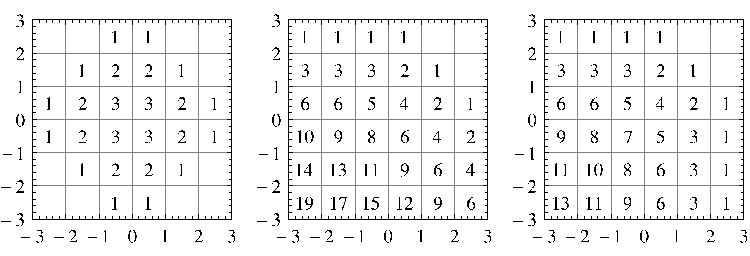
\includegraphics[width=130mm]{figures/irrep-verma-pverma}$
\end{lstlisting}

Как мы уже отмечали, свойства модулей определяются его сингулярным элементом. Функция  \lstinline{singularElement[m_module]} возвращает сингулярный элемент модуля в виде структуры данных  \lstinline{formalElement}. Характер  (вплоть до предела \lstinline{limit} для  (параболических) модулей Верма) вычисляется функцией \lstinline{character[m_module]}. Прямая сумма модулей является модулем и мы используем естественные обозначения
\begin{lstlisting}[mathescape=true]
im1=makeIrreducibleModule[$B_{2}$][weight[$B_{2}$][2,1]];
im2=makeIrreducibleModule[$B_{2}$][weight[$B_{2}$][1,2]];
textPlot[im1$\oplus$ im2]
$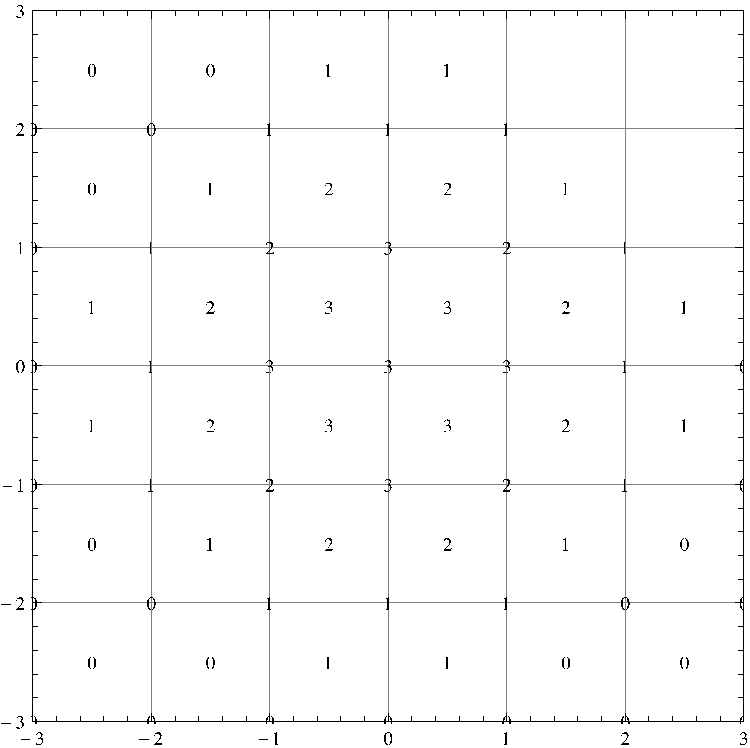
\includegraphics[width=60mm]{figures/irrep-sum}$
\end{lstlisting}

Тензорное произведение модулей тоже реализовано, но только для модулей конечномерных алгебр Ли. Это связано с тем, что тензорные произведения модулей аффинных алгебр Ли приводят к возникновению различных дополнительных структур  \cite{kazhdan1994tensor3,kazhdan1993tensor1,kazhdan1993tensor2}, изучение которых пока лежит за пределами наших интересов. 
\begin{lstlisting}[mathescape=true]
textPlot[makeIrreducibleModule[$A_{1}$][5]$\otimes$ makeIrreducibleModule[$A_{1}$][3]];
$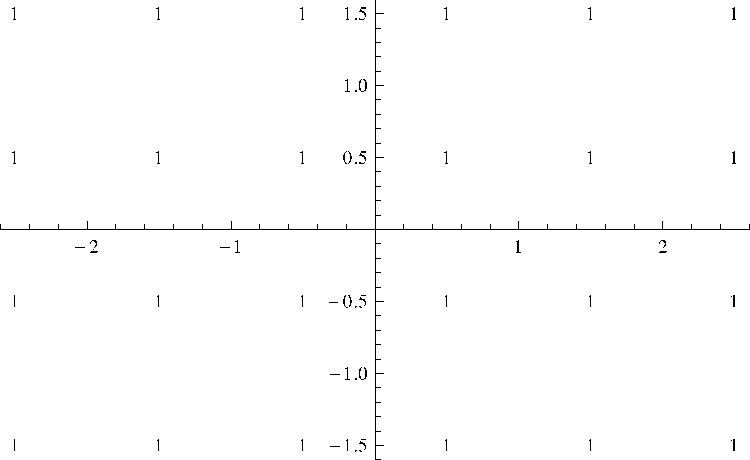
\includegraphics[width=60mm]{figures/tensor-product}$
\end{lstlisting}
\section{Основные алгоритмы}
\label{sec:comp-algor}
   
Существует два рекуррентных соотношения \eqref{eq:15}, \eqref{eq:14}, которые можно использовать для вычисления кратностей весов в неприводимых модулях. Оба алгоритма состоят из следующих шагов:
\begin{enumerate}
\item Построение списка весов в главной камере Вейля путем вычитания всех возможных комбинаций простых корней их старшего веса (например, для конечномерной алгебры вычитаем корень  $\alpha_{1}$ из старшего веса $\mu$ до тех пор, пока остаемся внутри  $\bar C$, затем вычитаем корень $\alpha_{2}$ из всех весов полученных на перво шаге и так далее).
\item Сортировка списка весов по значению их скалярного произведения с вектором Вейля.
\item Рекуррентное вычисление кратностей по формуле. Если вес, необходимый для вычислений оказывается вне главной камеры Вейля, то используется симметрия относительно группы Вейля.
\end{enumerate}
Различие в производительности алгоритмов происходит от количества предыдущих значений, требующихся для вычисления кратности веса. В случае рекуррентного соотношения, основанного на формуле Вейля  \eqref{eq:14} это количество постоянно и равно числу элементов в группе Вейля (если мы находимся далеко от внешнего контура диаграммы представления). При использовании формулы Фрейдентала \eqref{eq:15} требуемое число предыдущих значений растет с расстоянием от внешнего контура диаграммы представления.  Поэтому формула Фрейденталя работает быстрее, если вес близок к границе или ранг алгебры и размер группы Вейля велик \cite{moody1982fast}. Заметим, что формула Фрейденталя работает только для неприводимых модулей и не подходит для изучения (обобщенных) модулей Верма.

Мы осуществили тестирование производительности наших реализаций алгоритмов, основанных на формуле Фрейденталя и формуле \eqref{eq:15} и получили результаты, представленные на Рисунке  \ref{fig:freudenthal-racah-times}. Там показана зависимость времени вычислений от числа весов в модуле.

\begin{figure}[h]
  \noindent\centering{
    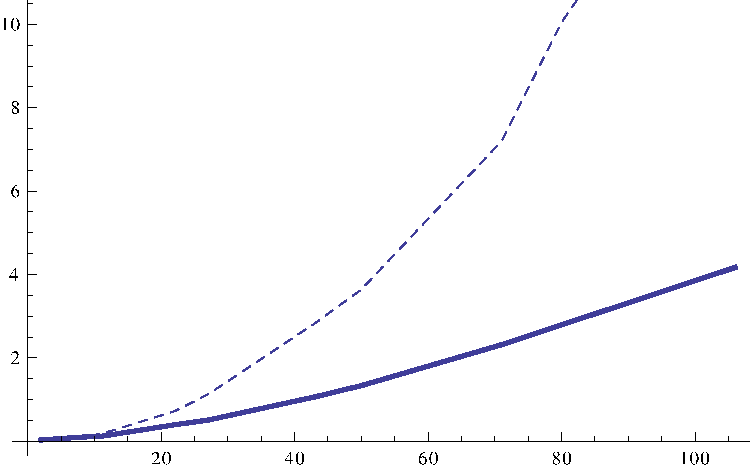
\includegraphics[width=80mm]{figures/timing}
  }
  \caption{Время работы алгоритмов, основанных на формуле Фрейденталя \eqref{eq:15} (пунктир) и рекуррентном соотношении \eqref{eq:14} (сплошная линия) в зависимости от количества весов в  $\bar C$ для вычисления кратностей в представлениях алгебры $B_{2}$.}
\label{fig:freudenthal-racah-times}

\end{figure}

При вычислении коэффициентов ветвления использование формулы Фрейденталя требует полного построения формальных характеров представления алгебры и всех представлений подалгебры, входящих в его разложение. Такой подход становится непрактичным для большого ранга алгебры и подалгебры, например, при максимальных вложениях. 

Альтернативный алгоритм описан в разделе \ref{sec:algorithm}. Рассмотренный там же пример регулярного вложения \ref{sec:someth-high-dimens}  $B_{2}\subset B_{4}$ позволяет сделать следующее сравнение числа требующихся операций. В данном примере веер вложения состоит из 24 элементов. Для разложения модуля алгебры  $B_{4}$ необходимо построить подмножество сингулярных весов модуля, проектирующихся в главную камеру Вейля подалгебры $B_{2}$. Полное множество сингулярных весов состоит из 384 элементов, в главную камеру Вейля проектируется не более 48, так что время на построение этого множества пренебрежимо мало, если число коэффициентов ветвления более 48. Мы можем оценить сверху общее число операций для вычисления коэффициентов ветвления произведением числа весов в главной камере Вейля подалгебры с ненулевыми коэффициентами ветвления на число элементов веера вложения. 
С другой стороны, при использовании алгоритма, основанного на построении всех характеров при помощи формулы Фрейденталя мы должны вычислить кратности для каждого модуля в разложении, так что общее количество операций растет с ростом числа весов в представлении быстрее, чем квадрат числа весов в главной камере Вейля подалгебры с ненулевыми коэффициентами ветвления. 

Чтобы проиллюстрировать эту разницу в производительности алгоритмов, мы приводим Рисунок \ref{fig:branching}, на котором показано время, необходимое для вычисления коэффициентов ветвления для вложения $B_{3}\subset B_{4}$.

\begin{figure}[h]
  \noindent\centering{
   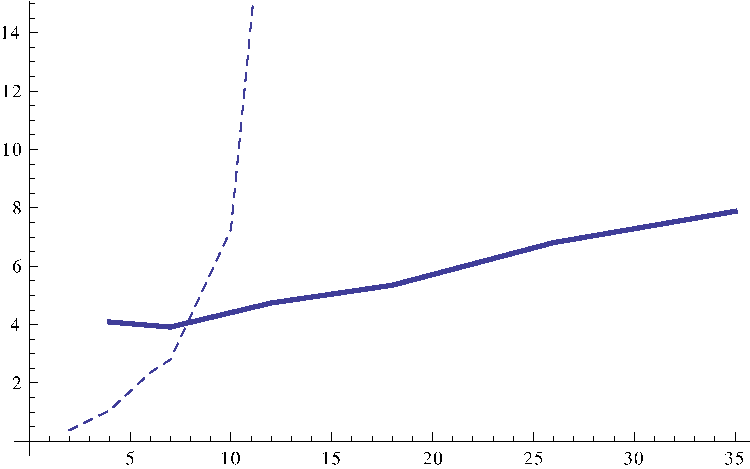
\includegraphics[width=100mm]{figures/branching-timing}
  }
  \caption{Время работы алгоритмов, основанных на применении формулы Фрейденталя \eqref{eq:15} (пунктиром)  и рекуррентного соотношения \eqref{recurrent-relation} (сплошная линия) с ростом числа весов в  $\bar C$ при вычислении коэффициентов ветвления для вложения $B_{3}\subset B_{4}$.}
  \label{fig:branching}
\end{figure}

\section{Примеры}
\label{sec:examples-six}
В этом разделе мы приводим примеры вычислений, проведенных с использованием {\bf Affine.m} и код, который для этого потребовался.

\subsection{Разложение тензорных произведений модулей конечномерных алгебр Ли на неприводимые}
\label{sec:tens-prod-decomp}

Вычисление коэффициентов слияния для разложения тензорного произведения модулей старшего веса в прямую сумму неприводимых модулей важно для различных приложений в физике. Например, мы можем рассматривать спин составной системы, такой как атом. Другой интересный пример -- это интегрируемые спиновые цепочки, состоящие из  $N$ частиц со спинами, живущими в некотором представлении  $L$ алгебры Ли $\gf$, с  $\gf$-инвариантным гамильтонианом $H$, описывающим спин-спиновое взаимодействие ближайших соседей. Чтобы решить такую систему, то есть найти собственные состояния гамильтониана, мы должны разложить  $L^{\otimes N}$ в прямую сумму неприводимых $\gf$-модулей меньшей размерности и диагонализовывать гамильтониан на этих модулях.

Для фундаментальных представлений простых алгебр Ли иногда можно написать аналитический ответ, описывающий зависимость коэффициентов разложения от  $N$ (См. работу \cite{LyakhovskyPostnova2011}). Наш код позволяет получать численные ответы, которые можно использовать для проверки этих аналитических результатов.

Рассмотрим тензорную степень $\left(L^{[1,0]}\right)^{\otimes 4}$ первого фундаментального представления алгебры $B_{2}$. Коэффициенты разложения тензорной степени на неприводимые модули -- это коэффициенты ветвления модуля алгебры $B_{2}\oplus B_{2}\oplus B_{2}\oplus B_{2}$ на диагональную подалгебру $B_{2}\subset B_{2}\oplus B_{2}\oplus B_{2}\oplus B_{2}$. Следующий код осуществляет необходимые вычисления:
\begin{lstlisting}[mathescape=true]
fm = makeIrreducibleModule[$B_{2}$][1, 0];
tp = ((fm$\otimes$ ]fm)$\otimes$ fm)$\otimes$]fm;
subs = makeFiniteRootSystem[
  {1/4*{1, -1, 1, -1, 1, -1, 1, -1}, 
   1/4*{0, 1, 0, 1, 0, 1, 0, 1}}];
bc = branching[tp, subs];
{bc[#], dynkinLabels[subs][#]} & /@ bc[weights]
\end{lstlisting}
Он выдает в результате следующий набор старших весов и коэффициентов разложения:
\begin{lstlisting}
{{1, {4, 0}}, {3, {2, 2}}, {0, {3, 0}}, 
{2, {0, 4}}, {3, {1, 2}}, {6, {2, 0}}, 
{6, {0, 2}}, {1, {1, 0}}, {3, {0, 0}}}]
\end{lstlisting}

Возвращаясь к проблеме диагонализации гамильтониана спиновой цепочке, мы можем заметить, что вместо диагонализации оператора в пространстве размерности  $625$ мы можем диагонализовывать операторы в пространствах размерностей $55, 81, 30, 35, 35, 14, 10, 5, 1$.

\subsection{Ветвления и параболические модули Верма}
\label{sec:branch-parab-verma}

Мы иллюстрируем обобщенную резольвенту Бернштейна-Гельфанда-Гельфанда (см. главу \ref{cha:BGG}) диаграммами параболических модулей Верма алгебры $G_{2}$, возникающих в разложении неприводимого модуля $L^{[1,1]}_{G_{2}}$:
\begin{equation}
\mathrm{ch}\left( L^{\mu }\right) =\sum_{u\in U}\;e^{\mu _{\aft}\left(
u\right) }\epsilon (u)\mathrm{ch}M_{I}^{\mu _{\frak{a}_{\perp }}\left(
u\right) }.  \label{char-in-gen-verma-mod}
\end{equation}
Характер  $L^{[1,1]}$ представлен на Рисунке \ref{branching-bgg}, характеры обобщенных модулей Верма в разложении  \eqref{char-in-gen-verma-mod} показаны на Рисунке  \ref{g2-pverma}. Характеры в верхнем ряду входят в формулу \eqref{char-in-gen-verma-mod} со знаком плюс, в нижнем -- со знаком минус. 


\begin{figure}[h]
  \noindent\centering{
    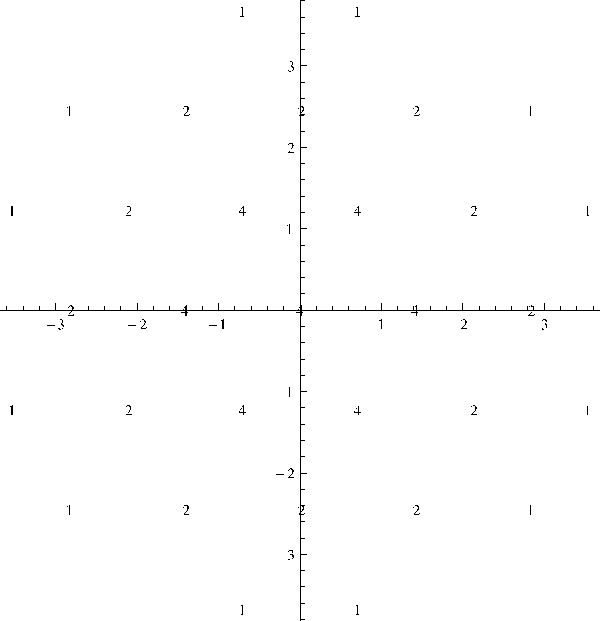
\includegraphics[width=80mm]{figures/G2-irrep}
  }
  \caption{Характер неприводимого модуля  $L^{[1,1]}$ алгебры $G_{2}$}
  \label{branching-bgg}
\end{figure}
\begin{figure}[h]
  \noindent\centering{
    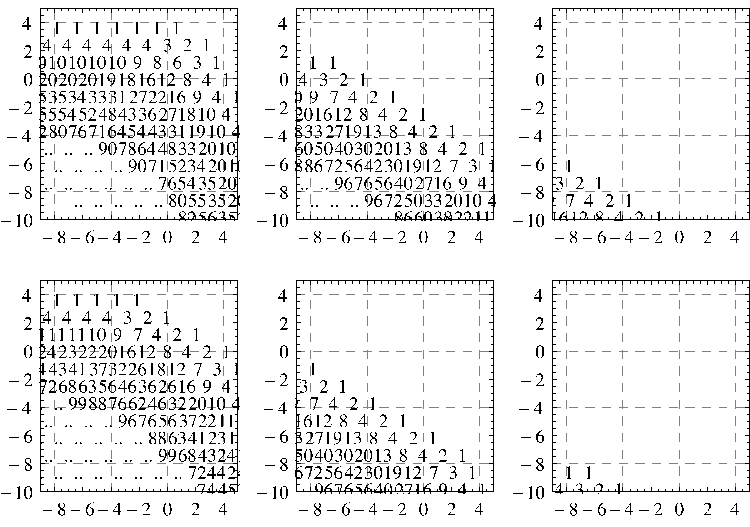
\includegraphics[width=150mm]{figures/G2-pverma}
  }
  \caption{Характеры обобщенных модулей Верма алгебры $G_{2}$, входящие в разложение характера $L^{[1,1]}$. Параболические модули Верма в верхнем ряду входят в разложение со знаком плюс, в нижнем -- со знаком минус.}
  \label{g2-pverma}
\end{figure}

\subsection{Струнные функции аффинных алгебр Ли и модели конформной теории поля}
\label{sec:string-funct-affine}
Струнные функции можно использовать для описания формальных характеров представлений старшего веса аффинных алгебр Ли. Эти функции обладают интересными аналитическими и модулярными свойствами \cite{kac1990idl,kac1988modular,kac1984infinite}.

{\bf Affine.m} позволяет вычислять степенное разложение для струнных функций. Рассмотрим аффинную алгебру Ли $\hat{sl(3)}=\hat A_{2}$ и ее модуль старшего веса $L^{(1,0,0)}$. Чтобы получить струнные функции используем следующий код:
\begin{lstlisting}[mathescape=true]
stringFunctions[$\hat A_2$,{1,1,2}]
{{0, 0, 4}, 
  $2 q + 10 q^2 + 40 q^3 + 133 q^4 + 398 q^5 + 1084 q^6 + 2760 q^7 + 6632 q^8 + 15214 q^9 + 33508 q^{10}$}, 
{{0, 3, 1}, 
  $2 q + 12 q^2 + 49 q^3 + 166 q^4 + 494 q^5 + 1340 q^6 + 3387 q^7 + 8086 q^8 + 18415 q^9 + 40302 q^{10}$}, 
{{1, 1, 2}, 
  $1 + 6 q + 27 q^2 + 96 q^3 + 298 q^4 + 836 q^5 + 2173 q^6 + 5310 q^7 + 12341 q^8 + 27486 q^9 + 59029 q^{10}$}, 
{{2, 2, 0}, 
  $1 + 8 q + 35 q^2 + 124 q^3 + 379 q^4 + 1052 q^5 + 2700 q^6 + 6536 q^7 + 15047 q^8 + 33248 q^9 + 70877 q^{10}$}, 
{{3, 0, 1}, 
  $2 + 12 q + 49 q^2 + 166 q^3 + 494 q^4 + 1340 q^5 + 3387 q^6 + 8086 q^7 + 18415 q^8 + 40302 q^9 + 85226 q^{10}$}
\end{lstlisting}
Аналогично для аффинной алгебры Ли $\hat G_{2}$ получаем
\begin{lstlisting}[mathescape=true]
stringFunctions[$\hat G_2$,{1,1,0}]
{{2, 0, 0}, 
  $1 + 8 q + 37 q^2 + 138 q^3 + 431 q^4 + 1227 q^5 + 3208 q^6 + 7901 q^7$}, 
{{0, 0, 1}, 
  $3 q + 18 q^2 + 73 q^3 + 247 q^4 + 736 q^5 + 2000 q^6 + 5070 q^7$}, 
{{1, 1, 0},
  $1 + 7 q + 32 q^2 + 117 q^3 + 370 q^4 + 1055 q^5 + 2780 q^6 + 6880 q^7$}, 
{{0, 2, 0}, 
  $3 q + 15 q^2 + 63 q^3 + 210 q^4 + 633 q^5 + 1725 q^6 + 4407 q^7$}
\end{lstlisting}

\subsection{Функции ветвления и  coset-модели конформной теории поля}
\label{sec:branch-funct-coset}

Считается, что рациональные модели конформной теории поля могут быть получены как  $G/A$ coset-модели, соответствующие вложениям $\af\subset\gf$. Эти модели можно реализовать как калибровочные теории  \cite{Hwang:1994yr, hwang1993brst} (см. раздел \ref{sec:coset-models-cft}). 

Функции ветвления для вложения  $\af\subset\gf$ являются статсуммами для моделей конформной теории поля на торе (см. \cite{difrancesco1997cft}).

В качестве первого примера мы демонстрируем вычисление функций ветвления для вложения $\hat A_{1}\to \hat B_{2}$ до десятого грейда:
\begin{lstlisting}[mathescape=true]
branchingFunctions[$\hat B_{2}$,makeAffineExtension[makeFiniteRootSystem[{{1, 1}}]], {1, 1, 1}]

 {{3, 0}, 
  $2 + 14 q + 52 q^2 + 154 q^3 + 410 q^4 + 994 q^5 + 2248 q^6 + 4832 q^7 + 9934 q^8 + 19680 q^9 + 37802 q^{10}$},
 {{2, 1}, 
  $4 + 20 q + 72 q^2 + 220 q^3 + 584 q^4 + 1424 q^5 + 3248 q^6 + 7012 q^7 + 14488 q^8 + 28844 q^9 + 55616 q^{10}$},
 {{0, 3}, 
  $4 q + 20 q^2 + 68 q^3 + 200 q^4 + 516 q^5 + 1224 q^6 + 2736 q^7 + 5808 q^8 + 11820 q^9 + 23236 q^{10}$},
 {{1, 2}, 
  $2 + 14 q + 54 q^2 + 168 q^3 + 462 q^4 + 1148 q^5 + 2656 q^6 + 5812 q^7 + 12130 q^8 + 24358 q^9 + 47328 q^{10}$}
\end{lstlisting}

Второй пример -- это вычисление функций ветвления для регулярного вложения  $\hat B_{2}\subset \hat C_{3}$:
\begin{lstlisting}[mathescape=true]
sub=makeAffineExtension[parabolicSubalgebra[$C_{3}$][2,3]];
branchingFunctions[$\hat C_{3}$,sub, {2, 0, 0, 0}]

{{0, 1, 0}, 
  $2 q - 20 q^3 + 24 q^4 + 82 q^5 - 320 q^6 + 108 q^7$}, 
{{1, 0, 0}, 
  $1 - q - 8 q^2 + 19 q^3 + 16 q^4 - 156 q^5 + 205 q^6 + 640 q^7$}, 
{{0, 0, 1}, 
  $q - 5 q^3 + 7 q^5$}
\end{lstlisting}

\section*{Выводы к шестой главе}
\label{sec:6-conclusion}
В данной главе мы представили пакет {\bf Affine.m} для вычислений в теории представлений конечномерных и аффинных алгебр Ли. Он может использоваться для изучения групп Вейля, корневых систем, неприводимых модулей, модулей Верма и параболических модулей Верма конечномерных и аффинных алгебр Ли. Кроме того, мы обсудили основные идеи в реализации пакета  {\bf Affine.m}. 

Мы показали, что рекуррентный подход, основанный на формуле Вейля для характеров полезен не только для вычислений, но и позволяет прояснить связь с (обобщенной) резольвентой Бернштейна-Гельфанда-Гельфанда.

Также мы представили примеры вычислений с применением нашего пакета, полезных для различных физических и математических проблем. 

В следующих версиях программы мы планируем реализовать работу со скрученными аффинными алгебрами Ли, расширенными аффинными алгебрами и реализовать более полную поддержку вычислений коэффициентов разложения тензорных произведений.

\appendix

\section*{Описание пакета}
\label{package}
Пакет может быть бесплатно загружен с сайта \url{http://github.com/naa/Affine}. Чтобы получить разрабатываемую версию кода можно использовать систему управления версиями {\it git} и команду
\begin{lstlisting}[language=bash]
 git clone git://github.com/naa/Affine.git
\end{lstlisting}

%%  Содержимое пакета:
%%  \begin{verbatim}
%%      Affine/                              Корневой каталог
%%        demo/                               Демонстрации
%%          demo.nb                                Демонстрационный файл
%%          paper.nb                               Код, содержащийся в статье 
%%        doc/                                 Каталог документации
%%          figures/                             рисунки в статье
%%            timing.pdf                           диаграмма, показывающая производительность
%%            branching-timing.pdf                 ...  для коэффициентов ветвления
%%            irrep-sum.pdf                        сумма неприводимых представлений B2
%%            irrep-verma-pverma.pdf               неприводимое представлений, модуль Верма и обобщенный модуль Верма для B2
%%            G2-irrep.pdf                         неприводимое представление G2
%%            G2-pverma.pdf                        параболический модуль Верма для G2
%%            tensor-product.pdf                   тензорное произведение модулей  A1
%%          bibliography.bib                     Библиографическая база
%%          paper.pdf                            Статья, описывающая пакет
%%          paper.tex                            Исходный LaTeX-файл статьи
%%          TODO.org                             Список доработок
%%        src/                                 Каталог исходного кода
%%          affine.m                             основной пакет
%%        tests/                               Каталог тестов
%%          tests.m                              тесты
%%        README.markdown                    Инструкция по установке и использованию
%%  \end{verbatim}
%%  

%%  
%% References
%%
%% Following citation commands can be used in the body text:
%% Usage of \cite is as follows:
%%   \cite{key}         ==>>  [#]
%%   \cite[chap. 2]{key} ==>> [#, chap. 2]
%%

%% References with bibTeX database:

  %   \section*{References}
  %   \label{sec:references}
  %   
  %   
  %   \bibliography{bibliography}
  %   \bibliographystyle{phcpc}
  %   %\bibliographystyle{model1-num-names}
  %   
  %   
  %   %% Authors are advised to submit their bibtex database files. They are
  %   %% requested to list a bibtex style file in the manuscript if they do
  %   %% not want to use elsarticle-num.bst.
  %   
  %   %% References without bibTeX database:
  %   
  %   % \begin{thebibliography}{00}
  %   
  %   %% \bibitem must have the following form:
  %   %%   \bibitem{key}...
  %   %%
  %   
  %   % \bibitem{}
  %   
  %   % \end{thebibliography}
  %   
  %   
  %   

%%
%% End of file
%%% Local Variables: 
%%% mode: latex
%%% TeX-master: "thesis"
%%% End: 

%\conclusion
\label{cha:conclusion1}



%%
%% End of file
%%% Local Variables: 
%%% mode: latex
%%% TeX-master: "thesis"
%%% End: 

% ----------------------------------------------------------------
\bibliography{bibliography}
\bibliographystyle{utphys}
% ----------------------------------------------------------------
\appendix
%\input{app-a}
\end{document}
   %%%   
   %%%   
   %%%   % \documentclass[12pt]{disser}
   %%%   % \usepackage[russian]{babel}
   %%%   % \usepackage[utf8]{inputenc}
   %%%   % \usepackage{amssymb}
   %%%   
   %%%   %%%%%%%%%%%%%%%%%%%%%%%%%%%%%%%%%%%%%%%%%%%%%%%%%%%%%%%%%%%%%%%%%%%%%%%%%%%%%%%%%%%%%%%%%%%%%%%%%%%%
   %%%   \usepackage{amsmath}
   %%%   \usepackage{amsmath,amssymb,amsthm}
   %%%   \usepackage{multicol}
   %%%   \usepackage{color}
   %%%   \usepackage{graphicx}
   %%%   \usepackage{hyperref}
   %%%   
   %%%   \newtheorem{statement}{Statement}
   %%%   \newtheorem{theorem}{Theorem}
   %%%   \newtheorem{corollary}{Corollary}[theorem]
   %%%   \newtheorem{lemma}{Lemma}
   %%%   \newtheorem{mynote}{Note}[section]
   %%%   \theoremstyle{definition}
   %%%   \newtheorem{definition}{Definition}
   %%%   \newtheorem{remark}{Remark}
   %%%   \newtheorem{example}{Example}
   %%%   \newcommand{\go}{\stackrel{\circ }{\mathfrak{g}}}
   %%%   \newcommand{\ao}{\stackrel{\circ }{\mathfrak{a}}}
   %%%   \newcommand{\co}[1]{\stackrel{\circ }{#1}}
   %%%   \newcommand{\pia}{\pi_{\mathfrak{a}}}
   %%%   \newcommand{\piab}{\pi_{\mathfrak{a}_{\bot}}}
   %%%   \newcommand{\gf}{\mathfrak{g}}
   %%%   \newcommand{\af}{\mathfrak{a}}
   %%%   \newcommand{\aft}{\widetilde{\mathfrak{a}}}
   %%%   \newcommand{\afb}{\mathfrak{a}_{\bot}}
   %%%   \newcommand{\hf}{\mathfrak{h}}
   %%%   \newcommand{\hfb}{\mathfrak{h}_{\bot}}
   %%%   \newcommand{\pf}{\mathfrak{p}}
   %%%   %\input{tcilatex}
   %%%   
   %%%   \begin{document}
   %%%   \title{Бесконечномерные алгебры симметрии в моделях квантовой теории поля}
   %%%   \author{А.А. Назаров$^{1,2}$\\
   %%%   {\small $^1$ Theoretical Department, SPb State University}\\
   %%%   {\small 198904, Sankt-Petersburg, Russia}\\
   %%%   {\small$^{2}$ Chebyshev Laboratory,}\\
   %%%   {\small Department of Mathematics and Mechanics, SPb State University}\\
   %%%   {\small 199178, Saint-Petersburg, Russia}\\
   %%%   {\small email: antonnaz@gmail.com}}
   %%%   
   %%%   \maketitle
   %%%   
   %%%   \begin{abstract}
   %%%   \end{abstract}
   %%%   
   %%%   \tableofcontents
   %%%   
   %%%   \chapter{Введение}
   %%%   \label{cha:intro}
   %%%   
   %%%   
   %%%   
   %%%   \section{Обозначения}
   %%%   
   %%%   Пусть $\frak{g}$ и $\frak{a}$ -- (аффинные) алгебры Ли, и существует вложение  $\frak{a}\hookrightarrow \frak{g}$ такое, что  $\frak{a}$ -- редуктивная подалгебра в $\frak{g}$ с согласованным корневым пространством: $\frak{%
   %%%   h}_{\frak{a}}^{\ast }\subset \frak{h}_{\frak{g}}^{\ast }$. Мы используем следующие обозначения:
   %%%   
   %%%   $\frak{g=n}^{-}+\frak{h}+\frak{n}^{+}$ --- разложение Картана;
   %%%   
   %%%   $r$ , $\left( r_{\frak{a}}\right) $ --- ранг алгебра $\frak{g}$ $%
   %%%   \left( \mathrm{\text{соотв., }\frak{a}}\right) $ ;
   %%%   
   %%%   $\Delta $ $\left( \Delta _{\frak{a}}\right) $--- корневая система; $\Delta
   %%%   ^{+} $ $\left( \mathrm{\text{соотв., }\Delta _{\frak{a}}^{+}}\right) $--- набор положительных корней (алгебр $\frak{g}$ и $\frak{a}$ соответственно);
   %%%   
   %%%   $\mathrm{mult}\left( \alpha \right) $ $\left( \mathrm{mult}_{\frak{a}}\left(
   %%%   \alpha \right) \right) $ --- кратность корня $\alpha$ в $%
   %%%   \Delta $ (соотв., в $\left( \Delta _{\frak{a}}\right) $);
   %%%   
   %%%   $S\quad \left( S_{\frak{a}}\right) $ --- множество простых корней (для 
   %%%   $\gf$ и $\af$ соответственно);
   %%%   
   %%%   $\alpha _{i}$ , $\left( \alpha _{\left( \frak{a}\right) j}\right) $ ---  $%
   %%%   i$-й (соотв., $j$-й) простой корень алгебры $\frak{g}$ $\left( \mathrm{\text{соотв.,}\frak{a%
   %%%   }}\right) $; $i=0,\ldots ,r$,\ \ $\left( j=0,\ldots ,r_{\frak{a}}\right) $;
   %%%   
   %%%   
   %%%   $\alpha _{i}^{\vee }$ , $\left( \alpha _{\left( \frak{a}\right) j}^{\vee
   %%%   }\right) $-- простой ко-корень для $\frak{g}$ $\left( \mathrm{\text{соотв.,}\frak{a}%
   %%%   }\right) $ , $i=0,\ldots ,r$ ;\ \ $\left( j=0,\ldots ,r_{\frak{a}}\right) $;
   %%%   
   %%%   $W$ , $\left( W_{\frak{a}}\right) $--- группа Вейля;
   %%%   
   %%%   $C$ , $\left( C_{\frak{a}}\right) $--- фундаментальная камера Вейля;
   %%%   
   %%%   $\bar{C}, \left(\bar{C_{\frak{a}}}\right)$ --- замыкание фундаментальной камеры Вейля;
   %%%   
   %%%   $\epsilon \left( w\right) :=\left( -1\right) ^{\mathrm{length}(w)}$;
   %%%   
   %%%   $\rho $\ , $\left( \rho _{\frak{a}}\right) $\ --- вектор Вейля;
   %%%   
   %%%   $L^{\mu }$\ $\left( L_{\frak{a}}^{\nu }\right) $\ --- интегрируемый модуль  $\frak{g}$ со старшим весом $\mu $\ ; (соотв., интегрируемый $\af$-модуль старшего веса $\nu $);
   %%%   
   %%%   $\mathcal{N}^{\mu }$ , $\left( \mathcal{N}_{\frak{a}}^{\nu }\right) $ ---
   %%%   весовая диаграмма модуля $L^{\mu }$ (соотв., ${}L_{\frak{a}}^{\nu }$ );
   %%%   
   %%%   $P$ (соотв., $P_{\frak{a}} $) \ --- весовая решетка;
   %%%   
   %%%   $P^{+}$ (соотв., $P_{\frak{a}}^{+} $) \ --- решетка доминантных весов;
   %%%   
   %%%   $m_{\xi }^{\left( \mu \right) }$ , $\left( m_{\zeta }^{\left( \nu \right)
   %%%   }\right) $ --- кратность веса $\xi \in P$ \ $\left( \mathrm{\text{соотв., }\in P_{\frak{a}}}\right) $ в $L^{\mu }$, (соотв., в $\zeta \in
   %%%   L_{\frak{a}}^{\nu } $);
   %%%   
   %%%   $ch\left( L^{\mu }\right) $ (соотв., $\mathrm{ch}\left( L_{\frak{a}}^{\nu
   %%%   }\right) $)--- формальный характер $L^{\mu }$ (соответственно, $L_{\frak{a}}^{\nu
   %%%   } $);
   %%%   
   %%%   $ch\left( L^{\mu }\right) =\frac{\sum_{w\in W}\epsilon (w)e^{w\circ (\mu
   %%%   +\rho )-\rho }}{\prod_{\alpha \in \Delta ^{+}}\left( 1-e^{-\alpha }\right) ^{%
   %%%   \mathrm{{mult}\left( \alpha \right) }}}$ --- формула Вейля-Каца;
   %%%   
   %%%   $R:=\prod_{\alpha \in \Delta ^{+}}\left( 1-e^{-\alpha }\right) ^{\mathrm{{%
   %%%   mult}\left( \alpha \right) }}\quad $ (соотв., $R_{\frak{a}}:=\prod_{\alpha \in
   %%%   \Delta _{\frak{a}}^{+}}\left( 1-e^{-\alpha }\right) ^{\mathrm{mult}_{\frak{a}%
   %%%   }\left( \alpha \right) } $)--- знаменатель Вейля.
   %%%   
   %%%   \chapter{Аффинные алгебры Ли}
   %%%   
   %%%   \section{Конечномерные алгебры Ли}
   %%%   \label{sec:finite-dimensional}
   %%%   Основные определения: корни, веса, кратности.
   %%%   
   %%%   \section{Теория представлений аффинных алгебр Ли}
   %%%   \label{sec:representation-theory}
   %%%   Определение аффинных алгебр. Корни, веса, кратности. Категория О.
   %%%   
   %%%   \section{Ветвления}
   %%%   Веер вложения. Алгоритм.
   %%%   
   %%%   \section{БГГ-резольвента}
   %%%   \label{sec:bgg}
   %%%   Категория О.
   %%%   Резольвента Бернштейна-Гельфанда-Гельфанда для представлений аффинных алгебр Ли. Параболические модули и их связь с подалгебрами и ветвлением.
   %%%   
   %%%   
   %%%   
   %%%   
   %%%   \section{Проблемы вычислений}
   %%%   \label{sec:computations}
   %%%   Производительность, скорость алгоритмов. 
   %%%   
   %%%   \chapter{Конформная теория поля}
   %%%   \label{cha:cft}
   %%%   
   %%%   Подробное изложение \cite{difrancesco1997cft}. 
   %%%   
   %%%   \section{Общие свойства}
   %%%   \label{sec:cft-general}
   %%%   Алгебра Вирасоро. Представления алгебры Вирасоро. Модулярная инвариантность.
   %%%   
   %%%   \section{Модели Весса-Зумино-Новикова-Виттена}
   %%%   \label{sec:wzw}
   %%%   Связь с аффинными алгебрами Ли.
   %%%   Конформные вложения и недиагональные модулярные инварианты. 
   %%%   
   %%%   \section{Coset-модели}
   %%%   Ветвления. Функции ветвления и статсуммы. 
   %%%   Калибровочные WZW-модели. 
   %%%   
   %%%   \section{SLE}
   %%%   \label{sec:sle}
   %%%   SLE на WZW-моделях. Граничные условия. Парафермионы. SLE на coset-моделях.
   %%%   
   %%%   \chapter{Заключение}
   %%%   \label{cha:conclusion}
   %%%   
   %%%   
   %%%   \bibliography{bibliography}{}
   %%%   \bibliographystyle{utphys}
   %%%   
   %%%   \end{document}

%%% Local Variables: 
%%% mode: latex
%%% TeX-master: t
%%% End: 
